\documentclass{article}
\usepackage[UTF8]{ctex}
\usepackage{amsmath}
\usepackage{amsfonts}
\usepackage{mathtools}
\usepackage{jadamath}
\usepackage{hyperref}
% \usepackage[colorlinks=true,linkcolor=blue]{hyperref}
\usepackage{esint}
\usepackage{bm}
\usepackage{braket}
\usepackage{graphicx}
\usepackage{xcolor}
\usepackage{fancyhdr}
\usepackage{geometry}
\usepackage{float}
\usepackage{color}
\usepackage{enumitem}
\usepackage{ulem}
\usepackage{physics}
\usepackage{extarrows}
\usepackage{hyperref}
\usepackage[Symbol]{upgreek}
\usepackage[adjust]{cite}
%opening
\newcommand{\pic}[1]{\begin{wrapfigure}{l}[30cm]{0pt}%
		\includegraphics[width=40mm]{#1}%
\newcommand{\one}{1}
\end{wrapfigure}}
\newgeometry{top=25mm,bottom=25mm,left=30mm,right=30mm}
\title{\textbf{北京大学2019学年春季《量子力学A》课程习题解答}\\\vspace{2mm}汇总版}
\author{李聪乔 高学诗}
\date{\today}
\begin{document}

\maketitle
\tableofcontents
\newpage
\section{第一章“物质波概念的建立与物质波的描述方案”习题解答}
{下为根据刘老师量子力学讲义第一章作业制作的习题解答。请大家尤其重点看一下1.4, 1.8, 1.13, 1.24, 1.31, 1.32, 1.38, 1.40, 1.41题及红字标注的部分,这是大家出错率较高的及我们认为有必要提醒大家的重点题目。周五习题课上我们会讲解部分习题。}

常用物理量:$ \sigma=5.6704\ten{-8}\;\mathrm{J/(K^4\cdot s\cdot m^2)} $,
$ h = 6.6261\ten{-34}\;\mathrm{kg\cdot m^2/s} $,
$ hc=1240\;\mathrm{eV\cdot nm} $

\begin{enumerate}[label=1.\arabic*, leftmargin=-0.5mm]

\item 
黑色平板吸收与辐射平衡
$ E_{in}=E_{a}= 1350\; \mathrm{J/(s\cdot m^2)}$。
将平板视为黑体,由Stefan-Boltzmann定律有
\[E_{in}=2\sigma T^4.\]
{\color{red}注意到因平板有两面,所以要加一个因子\,2}。解得$ T=330\;\mathrm{K} = 57\ssd $。

\item
地球上$ S_0=1\cm^2 $的区域于$T_0=60\s$接受辐射能量$E_0=8.11\;\mathrm{J}$ ,
太阳光的能流密度为\[E=\frac{4\_pi L^2}{4\pi(D/2)^2}\cdot \frac{E_0}{S_0T_0} \]
太阳温度为5778 K,则由Stefan-Boltzmann定律可求得
\[\sigma = \frac{4\pi L^2}{4\pi(D/2)^2}\cdot \frac{E_0}{S_0T_0}\cdot \frac{1}{T^4}=5.65\ten{-8}\;\mathrm{J/(K^4\cdot s\cdot m^2)}.\]

\item
波长在550 nm到551 nm内可认为辐射功率随波长变化很小,因此
\[P\approx r_B(\lambda,\;T)\Delta \lambda\cdot S.\]
由普朗克公式
\[r_B(\lambda,\;T) = \frac{2\pi hc^2}{\lambda^5}\frac{1}{e^{\frac{hc}{\lambda k_B T}-1}}.\]
并代入$\lambda=1.0\nm$,$S=\pi(D/2)^2$,$T=5973\kai$得到$P=7.40\ten{-4}\;\mathrm{W}$。

单位时间内光子发射数目为
\[N = \frac{P}{hc/\lambda} = 2.05\ten{15}\;\text{个/s}.\]

\item
(1) 求辐射场温度。{\color{red}对光子场,能量密度$U$与能流密度$J$满足$J=\frac{1}{4}cU$}。现简要推导如下(详见热力学统计物理教材):

考虑辐射场中射向$\dd{A}$小面元的辐射能量。在$\dd{\Omega}$立体角内单位时间射向面元的能量为$cU\cos\theta\dd{A}\frac{\dd{\Omega}}{4\pi}$,$\theta$为辐射方向与面元法线夹角。对立体角在面元一侧的半空间积分得
\[J\dd{A} = \int\frac{cU\dd{A}\cos\theta}{4\pi}\dd{\varOmega} = \frac{cU\dd{A}}{4\pi}\int_0^{\frac{\pi}{2}}\cos\theta\sin\theta\dd{\theta}\int_0^{2\pi}\dd{\varphi}=\frac{cU\dd{A}}{4}.\]
考虑在该辐射场中的黑体,达到热平衡时温度为$T$,此时应有辐射能量等于吸收的场能,故
\[J=\frac{1}{4}cU=\sigma T^4.\]
得到$T = 2.82\kai$,此即微波背景辐射的温度。

(2) 求光子数密度。辐射场的辐射能流$E(T)=\int_0^\infty r_B(\lambda,\;T )\dd{\lambda}$,其中$r_B(\lambda,\;T )$形式由普朗克公式给出。根据辐射能量与能流的关系,可知$\lambda$到$\lambda+\dd{\lambda}$区间内光子的能量密度为$u(\lambda,\;T)\dd{\lambda}= \frac 4c r_B(\lambda,\;T)\dd{\lambda}$,进一步可知光子数密度为
$n(\lambda,\;T)\dd{\lambda} = \frac{1}{hc/\lambda}u(\lambda,\;T)\dd{\lambda}$。
因此总光子数密度为
\[N(T)=\int_0^{\infty}n(\lambda,\;T)\dd{\lambda}=\int_0^{\infty}\frac{4\lambda}{hc^2}r_B(\lambda,\,T)\dd{\lambda} = \int_0^{\infty}\frac{8\pi}{\lambda^4}\frac{1}{e^{\frac{hc}{\lambda k_B T}}-1}\dd{\lambda}\]
换元$x=\frac{hc}{\lambda k_B T}$并作数值积分有
\[N(T)=8\pi \left(\frac{k_B T}{hc}\right)^3\int_0^\infty \frac{x^2}{e^x -1}\dd{x} = 2.404\times8\pi\left(\frac{k_B T}{hc}\right)^3,\]
代入温度$T$得到$N=4.5\ten{8}\;\mathrm{m^{-3}}$.

(注:本题可直接由统计物理中的光子气体分布推出。由玻色-爱因斯坦分布可导出与上面完全一致的形式。详见统计学课本。)

(3) 平均光子能量
\[\bar{\epsilon}=\frac{\int_0^{\infty}u(\lambda,\;T)\dd{\lambda}}{\int_0^{\infty}\frac{u(\lambda,\;T)}{hc/\lambda}\dd{\lambda}}=\frac{8\pi\frac{k_B^4 T^4}{h^3 c^3}\frac{\pi^4}{15}}{8\pi\left(\frac{k_B T}{hc}\right)^3\times 2.404} = \frac{\pi^4}{15\times2.404}k_B T,\]
代入温度得到$\bar\epsilon = 1.1\ten{-22}\;\mathrm{J}.$

(4) 由维恩位移定律可知最大亮度对应波长为$\lambda_M = b/T= 1.0\mm$。


\item
蓝光波长$400\sim 450 \nm$。
取$\lambda_M=400\nm$作为辐射峰值所在波长计算,由维恩位移定律$\lambda_M T=b=2.898\ten{-3}\;\mathrm{m\cdot K}$,得到$T=7.2\ten{3}\kai=7.0\ten{3}\ssd$

\item
考虑温度为$T = 1.0\ten{7}$,由维恩位移定律$\lambda_M T=b$
可得$\lambda_M = 0.29\nm$,
光子能量为$E=hc/\lambda_M=4.3\ten{3}\eV=6.9\ten{-16}\;\mathrm{J}$。

\item
将人视为高为$h=1.8$ m的圆柱形,截面周长以腰围估算,取
$L=1.0$ m。
故辐射面积为$S=hL$。
人体体表温度$T = 33.5\ssd$,由Stefan-Boltzmann定律求得
辐射功率为$P=S\sigma T^4= 9.0\ten{2}$ W。

\item
可以将能流密度各自在频率$\lambda$与波长$\nu$上写作积分形式:
\[E(T) = \int_0^{\infty}r_B'(\nu,\,T)\dd{\nu} = \int_0^{\infty}r_B(\lambda,\,T)\dd{\lambda}. \]
我们实际上要求的是$r_B'(\nu,\,T)$取极值时所对应的$\nu_m$的表达式。根据
\eqa{\lvert r_B'(\nu,\,T)\mathrm{d}\nu\rvert=\lvert r_B(\lambda,\,T)\mathrm{d}\lambda\rvert}
辐射强度随频率变化的关系为
\eqa{r_B'(\nu,\,T)=r_B(\lambda,\,T)\Big\lvert\frac{\mathrm{d}\lambda}{\mathrm{d}\nu}\Big\rvert}
波长和频率的关系为$\,\lambda=c/\nu$,故
\eqa{\Abs{\drv{\lambda}{\nu}}=\frac{c}{\nu^2}}
所以
\alg{r_B'(\nu,\,T)=&r_B(\lambda,\,T)\cdot\frac{c}{\nu^2}\\
=&\frac{2\pi h}{c^2}\frac{\nu^3}{\exp(\frac{h\nu}{\kb T})-1}}
我们需要求$\,r_B'(\nu,\,T)\,$的极大值点$\,\nu_m$,令$\,\prv{r_B(\nu,\,T)}{\nu}=0$,得到方程
\eqa{x\epow{x}-3\epow{x}+3=0}
其中$\,x=\frac{h\nu_m}{\kb T}$。数值解为
\eqa{x=2.82}
则维恩位移定律的频率形式为
\eqa{\nu_m=2.82\frac{\kb T}{h}}

{\color{red}(注:绝大多数同学使用了$\nu_m = c/\lambda_m$,错误地直接由维恩位移定律的波长形式得到频率形式。事实上$\nu_m$与$\lambda_m$对应的是完全不同的函数取极值下的频率与波长,该极值点也并不在同一个波长/频率区间内取得。另外,上面过程中的$r_B'(\nu,\,T)$与$r_B(\lambda,\,T)$也是完全不同的函数,并不是简单地替换了自变量。请一定注意。)}

\item
(1)由维恩位移定律,最敏感波长应为$\lambda_M= b/T_0 = 9.27\mum$.

(2)总频谱亮度可由Stefan-Boltzmann定律求得为$E=\sigma T^4$,故高出的百分比
\[\frac{E'-E_0}{E_0} = \frac{T'^4-T_0^4}{T_0^4} = 8.1\%\]

\item
单个光子能量为$\epsilon = \frac{hc}{\lambda}$。
设每秒进入眼睛光子数为$N$,则光强$\frac{N\epsilon}{S}>10^{-10}\;\mathrm{W/m^2}$。
求得$N>3.67\ten{3}\;\mathrm{s^{-1}}$.

\item
单个光子能量为$\epsilon = \frac{hc}{\lambda}$,单位时间粒子数为$N$。功率为$P = N\epsilon = 3.61\ten{-17}\;\mathrm{W} = 225\;\mathrm{eV/s}$。

\item
$\Delta t$时间内,照到镜面单位面积上的光子数为$N\Delta t$,则照到单位面积上光子的原动量为
\[p = N\Delta t\cdot \frac{h\nu}{c} = \frac{Nh\nu\Delta t}{c}.\]
动量改变量
$\Delta p = p-(-p) = 2p $.
根据牛顿定律,$\Delta p = P_\text{压强}\Delta t$,则
\[P_\text{压强} = \frac{2Nh\nu}{c}\]
如果考虑光子不是正入射,设入射角为$\,\theta$,显然单个光子动量变化为$\,\Delta p_1=2\frac{h\nu}{c}\cos\theta$,单位面积上入射的光子数为$\,N\Delta t\cos\theta$,故光子总动量的改变为
\eqa{\Delta p=\Delta p_1N\Delta t\cos\theta}
根据牛顿定律,压强为
\eqa{P_{压强}=\frac{2Nh\nu}{c}\cos^2\theta}

\item
考虑截面为$S$,长度为$L$的空间。单个光子能量$\epsilon = h\nu$,则单位时间内照在单位面积上的辐射能量
\[E = \frac{N\epsilon SL}{S\cdot l/c} = N\epsilon c.\]
已知$E=1\;\mathrm{J/(cm^2\cdot s)}$。

(1) 对于$\nu=1\;\mathrm{MHz}$的无线电波,计算得粒子数密度为
$N = 5.03\ten{22}\;\mathrm{m^{-3}}$。

(2) 对于$E=h\nu=1\MeV$的光子,计算得粒子数密度为
$N = 2.08\ten{7}\;\mathrm{m^{-3}}$。

{\color{red}(注:本题中不能单纯地仿效1.4题得出$E = \frac{N\epsilon c}{4}$。这是因为题目中强调了考察对象是“一束”电磁波,这说明所有光子都是同方向的。这与1.4题中“各向同性”的光子场不同。)}

\item%14
假设自由电子可以发生光电效应。假定一个光子(动量为$\,\mathbf{p}_1$)与一个自由电子(动量为$\,\mathbf{p}_2$)碰撞,电子吸收光子,动量变为$\,\mathbf{p}_3$,$\mathbf{p}_1\,$与$\,\mathbf{p}_3\,$的夹角为$\,\theta$,则有动量守恒和能量守恒两个方程:
\alg{p_3^2+p_1^2-2p_1p_3\cos\theta=&p_2^2\\
p_1c+\sqrt{p_2^2c^2+E_0^2}=&\sqrt{p_3^2c^2+E_0^2}}
其中$\,E_0\,$为电子的静质量能。整理可得
\eqa{p_3^2c^2\sin^2\theta=-E_0^2}
此式左边是非负数而右边是负数,显然不可能成立。故自由电子不可能完全吸收一个光子而产生光电效应。

【另解】若一个光子与电子发生作用,末态只有一个电子,则我们可以考虑末态电子的静止系。根据能量守恒
\[E_{e\text{初}} + E_\gamma = E_{e\text{末}} = m_e c^2.\]
而显然初态电子具有非零动量,即$E_{e\text{初}}>m_e c^2$,故上式不可能成立。

\item
红限波长$\lambda_0 = 600\nm$,则逸出功为$W=\frac{hc}{\lambda_0}$。
设某单色光波长$\lambda$,由光电效应原理
\[\frac{hc}{\lambda}-W = eU_0.\]
解得
\[\lambda=\frac{hc}{eU_0+hc/\lambda_0} = 272\nm.\]

\item
根据$\frac{hc}{\lambda}-W = eU_0$,变形为
\[U_0 = \frac{hc}{e}\cdot \frac{1}{\lambda}-\frac{W}{e}.\]
因此可知$U_0$与$\frac{1}{\lambda}$呈线性关系。作最小二乘法拟合可得到斜率$\frac{hc}{e} = 1217\;\mathrm{V\cdot nm}$。由此求得普朗克常量$h=6.50\ten{-34}\;\mathrm{J\cdot m}$。

\item
截止波长$\lambda_0$满足$\frac{hc}{\lambda_0}=W$,解得$\lambda_0 = 539\nm$。若采用$\lambda=680\nm$的波长,则$\frac{hc}{\lambda}-W<0$,故不能发生光电效应。

\item
考虑红光波长$\lambda=760\nm$,其单个光子能量为$\epsilon = \frac{hc}{\lambda}=2.62\ten{-19}\;\mathrm{J}>10^{-19}\;\mathrm{J}$.
故可以利用溴化银底版在红光下进行拍照。

\item
根据能守恒原理,反冲电子的动能来源于光子能量的损失,即$E_R = E_{\gamma,I}-E_{\gamma,R}$。
考虑到康普顿散射效应中,出射光子波长与入射光子波长满足
\[\lambda'-\lambda = \frac{h}{m_e c}(1-\cos\theta).\]
而入射光子能量为$E_{\gamma,I}=\frac{hc}{\lambda}$已知,则可求得出射电子动能为
\[E_R = \frac{hc}{\lambda}-\frac{hc}{\lambda'} = E_{\gamma,I} - \frac{E_{\gamma,I}}{1+\frac{E_{\gamma,I}}{m_e c^2}(1-\cos\theta)}.\]

\item
设出射电子动量大小为$p$,入射、出射光子频率为$\nu,\,\nu'$。根据过程前后竖直(垂直于入射光子速度方向)、水平动量守恒:
\[
\begin{cases}
p\sin\phi = \frac{h\nu'}{c}\sin\theta \\
p\cos\phi = \frac{h\nu}{c}-\frac{h\nu'}{c}\cos\theta
\end{cases}
\]
二式作比得
\[\cot\phi = \frac{\nu-\nu'\cos\theta}{\nu'\sin\theta}.\]
由于$\frac{1-\cos\theta}{\sin\theta} = \tan\frac{\theta}{2}$,同时根据康普顿效应的波长差公式可得频率关系式
\[\frac{\nu-\nu'}{\nu\nu'} = \frac{h}{m_e c^2}(1-\cos\theta),\]
从而
\[\cot\phi = \nu'\frac{1-\cos\theta}{\sin\theta}+\frac{\nu-\nu'}{\nu'\sin\theta} = \nu'\tan\frac{\theta}{2}+\frac{\nu\nu'(1-\cos\theta)\frac{h}{m_e c^2}}{\nu'\sin\theta} = (1+\frac{h\nu}{m_e c^2})\tan\frac{\theta}{2}.\]
即为所求。

\item
散射前、后光子能量为$E_\nu,\,E_\nu'$,则根据康普顿散射公式:
\[\Delta \lambda = \frac{hc}{E_\gamma'}-\frac{hc}{E_\gamma} = \frac{hc}{m_e c}(1-\cos\theta),\]
求解得$\theta=41.9\du$。

\item
已知光子散射角$\theta = 90\du$。由康普顿散射公式可求得
\[\lambda' = \lambda+\frac{h}{m_e c}(1+\cos\theta) = \frac{hc}{E_\nu}+\frac{h}{m_e c} = 2.53\;\mathrm{pm}.\]

\item
设题述$5.00\MeV$为入射电子的动能,记为$E_k$,出射光子能量记为$E_{\gamma_1},\,E_{\gamma_2}$,$E_{\gamma_1}$朝向入射电子方向,则有动量、能量守恒关系式:
\[
\begin{cases}
p = \frac{1}{c}\sqrt{(m_e c^2 + E_k^2)-m_e^2 c^4} = \frac{1}{c}(E_{\gamma_1}-E_{\gamma_2})
\\
2m_e c^2 + E_k = E_{\gamma_1}+E_{\gamma_2}
\end{cases}
\]
两式相加、相减得$E_{\gamma_{1,2}} = m_e c^2+\frac{E_k}{2} \pm \frac{1}{2}\sqrt{E_k(E_k+2m_e c^2)}$,计算得$E_{\gamma_1}=5.76\MeV$,$E_{\gamma_2}=0.268\MeV$。

\item
{\color{red}首先请注意,单个光子不可能湮灭为一对正负电子。}请同学们思考其中的原因(在近代物理知识范围内)。于是我们猜测题目本意为散射光子能量应至少大于两倍电子静质量,即$E_\gamma'>2m_e c^2$。
根据康普顿散射公式,有
\[\frac{h}{m_e c}(1-\cos\theta) = \frac{hc}{E_\gamma'}-\frac{hc}{E_\gamma} < \frac{hc}{E_\gamma'}<\frac{h}{2m_e c},\]
从而$\cos\theta>\frac{1}{2}$,即$\theta<60\du$。

\item
光子垂直出射,$\theta=90\du$,根据康普顿散射公式,偏移量
\[\Delta\lambda = \frac{h}{m_e c}(1-\cos\theta) = 2.42\;\mathrm{pm}.\]
出射光子能量为$E_\gamma' = \frac{hc}{\lambda+\Delta\lambda}$,已知$\gamma$射线波长为$0.00188\nm$,则入射光损失的能量占总能量比为
\[\frac{E_\gamma'-E_\gamma}{E_\gamma} - \frac{\frac{1}{\lambda}-\frac{1}{\lambda+\Delta\lambda}}{\frac{1}{\lambda}} = \frac{\Delta\lambda}{\lambda+\Delta\lambda} = 56.3\%.\]
反冲动能等于光子能量损失,即
\[E_R = E_\gamma-E_\gamma' = \frac{hc}{\lambda}-\frac{hc}{\lambda+\Delta\lambda} = 5.96\ten{-14}\J = 0.372\MeV.\]

\item
卢瑟福散射公式是对单一点状原子核散射粒子所形成的分布的描述。引入瞄准距离$b$为入射粒子到原子核的垂直距离,则$\theta \rightarrow 0$实际对应着$b \rightarrow \infty$,这表示入射在$b>b_0$无穷大横截面上的粒子理论上都可以被散射进$\theta < \theta_0$的区域内,这自然造成了$\dv{\sigma(\theta)}{\Omega}$在$\theta \rightarrow 0$的发散。然而实际中,散射粒子不仅受到一个原子核的散射作用,对于以某个原子核为参考的$b$较大的入射粒子定会受到其他原子核的影响。故处理实际问题中应对每个原子核加以作用域的限制,超出该作用域范围的粒子将由其它原子核主导其散射行为。

\item
(略)

\item
在质子最接近Au原子时,动能完全转化为电势能,则有
\[\frac{1}{4\pi\epsilon_0}\frac{Ze^2}{r} = E_k.\]
Au元素$Z=79$,求解得$r=56.8\fm$。考虑到质子与Au核的半径,我们有$r>r_p+r_\mathrm{Au} = 8.9\fm$,因此质子与Au核不能接触以发生核反应。

\item
产生该结果的主要原因是:质子实际具有质量,因此质子-电子体系应当作为两体模型计算。我们下面求解考虑质子质量的情况下对里德堡常量的修正。

设质子质量$M$,电子质量$m$,二者绕共同质心作圆周运动,距离为$r$。由牛顿第二定律
\[\frac{1}{4\pi\epsilon_0}\frac{e^2}{r^2} = \frac{mv^2}{\frac{rM}{M+m}}.\]
角动量的量子化条件为
\[L = mvr\frac{M}{M+m}+M\frac{vm}{M}\frac{rm}{M+m} = mvr = n\hbar.\]
因此$r$只能取分立值:
\[\frac{1}{r} = \frac{e^2 m}{4\pi\epsilon^2\hbar^2}\frac{M}{M+m}\]
总能量为
\[E = \frac{1}{2}mv^2+\frac{1}{2}M\frac{v^2m^2}{M^2}-\frac{1}{4\pi\epsilon_0}\frac{e^2}{r}, \]
化简为
\[E = -\frac{1}{2}\frac{1}{4\pi\epsilon_0}\frac{e^2}{r}.\]
代入分立取值的$r$,对比玻尔理论可知里德堡常量的修正应为
\[R' = R\frac{M}{M+m}.\]
考虑到质子与电子质量比$M/m=1836$,可以计算出修正后的里德堡常量与观测值在较高精度内一致。

(注:1.40题所讨论的相对论效应也会对里德伯常量产生修正,参考1.40题结论可知修正量$\frac{\Delta R}{R}\sim \alpha^2 
\approx\frac{1}{137^2}<\frac{1}{1836}$,小于因质子质量带来的修正,故相对论效应并不是主要影响因素。)

\item
考虑到氢原子由基态向上激发,由于
\[E_1(\frac{1}{1^2}-\frac{1}{3^2}) < 12.5\eV < E_1(\frac{1}{1^2}-\frac{1}{4^2}),\]
可知$12.5\eV$的电子可将其激发至$n=2$或$n=3$态。因此受激发的氢原子向低能态跃迁可发出波长为:
\alg{\lambda_{32} &= \frac{hc}{E_1}(\frac{1}{2^2} - \frac{1}{3^2})^{-1}=656.5\nm\\
\lambda_{31} &= \frac{hc}{E_1}(\frac{1}{1^2} - \frac{1}{3^2})^{-1}=102.6\nm\\
\lambda_{21} &= \frac{hc}{E_1}(\frac{1}{1^2} - \frac{1}{2^2})^{-1}=121.6\nm
}

\item
假设电子做半径为$\,r\,$的圆周运动。电子的经典的运动方程为
\eqa{\frac{mv^2}{r}=\frac{1}{4\pi\varepsilon_0r^2}\frac{Ze^2r^3}{R^3}}
由此可得角动量
\eqa{L=mvr=\sqrt{\frac{Ze^2m}{4\pi\varepsilon_0R^3}}r^2}
玻尔理论方法令角动量量子化,有
\eqa{L=\sqrt{\frac{Ze^2m}{4\pi\varepsilon_0R^3}}r^2=n\hbar}
可得
\eqa{r^2=n\hbar\sqrt{\frac{4\pi\varepsilon_0R^3}{Ze^2m}}}
电子受力与距离成正比,其圆周运动可视为两个互相垂直的简谐运动的叠加,其能级应为
\eqa{E_n=2\cdot\frac{1}{2}\frac{Ze^2}{4\pi\varepsilon_0R^3}r^2=n\hbar\sqrt{\frac{Ze^2}{4\pi\varepsilon_0R^3m}}}
由于电子在球内运动,$r^2<R^2$,我们可以确定$\,n\,$的范围:
\eqa{n<\frac{1}{\hbar}\sqrt{\frac{Ze^2mR}{4\pi\varepsilon_0}}}

\item
设$\,\beta=v/c$,由狭义相对论的速度变换可得两个氢原子的相对速度为
\eqa{v_r=\frac{v-(-v)}{1-v(-v)/c^2}=\frac{2\beta c}{1+\beta^2}}
在发出光子的氢原子的参考系中,光子频率为
\eqa{\nu=cR\Brak{1-\frac{1}{2^2}}=\frac{3}{4}cR}
由于多普勒效应,在接收光子的氢原子参考系中,光子频率为
\eqa{\nu'=\sqrt{\frac{1+v_r/c}{1-v_r/c}}\nu=\frac{1+\beta}{1-\beta}\nu}
另一方面,氢原子接收光子后跃迁到第二激发态,说明光子的频率为
\eqa{\nu'=cR\Brak{1-\frac{1}{3^2}}=\frac{8}{9}cR=\frac{32}{27}\nu}
可见
\eqa{\frac{1+\beta}{1-\beta}=\frac{32}{27}}
解之得
\eqa{\beta=0.0862}
即速率$\,v=0.0862c$。\\
由于题目表述不清,也可将$\,v\,$理解为相对速度,此时有
\eqa{\nu'=\sqrt{\frac{1+\beta}{1-\beta}}\nu}
解得
\eqa{\beta=0.168}

\item
首先估算可见光区光子能量的范围,长波端和短波端分别约为
\alg{E_\mathrm{l}=&\frac{hc}{760\,\mathrm{nm}}=1.63\,\mathrm{eV}\\
E_\mathrm{s}=&\frac{hc}{380\,\mathrm{nm}}=3.26\,\mathrm{eV}}
莱曼系光子最低能量为
\eqa{E_\mathrm{ll}^\mathrm{L}=hcR\Brak{\frac{1}{1^2}-\frac{1}{2^2}}=10.2\,\mathrm{eV}>E_\mathrm{s}}
帕邢系光子最高能量为
\eqa{E_\mathrm{sl}^\mathrm{P}=hcR\Brak{\frac{1}{3^2}-\frac{1}{\infty^2}}=1.51\,\mathrm{eV}<E_\mathrm{l}}
可见氢原子光谱中位于可见光区的谱线均出自巴尔末系,$1/\lambda=R\Brak{\frac{1}{2^2}-\frac{1}{m^2}}$,计算出各可见光谱线波长如下表所示
\begin{table}[h]
    \centering
    \begin{tabular}{c|c}
    \hline
        \rule{0pt}{13pt}$m$ & $\lambda/\mathrm{nm}$\\
        \hline
        \rule{0pt}{13pt}3 & 656.3 \\
        \rule{0pt}{13pt}4 & 486.1 \\
        \rule{0pt}{13pt}5 & 434.1 \\
        \rule{0pt}{13pt}6 & 410.2 \\
        \rule{0pt}{13pt}7 & 397.0 \\
        \rule{0pt}{13pt}8 & 388.9 \\
    \hline
    \end{tabular}
    \caption{题\,1.33\,表}
\end{table}

\item
各谱系的长波极限波长为$\,n+1\,$态跃迁到$\,n\,$态对应的波长,各谱系的短波极限波长为$\,\infty\,$态跃迁到$\,n\,$态的波长。莱曼系对应$\,n=1$,巴尔末系对应$\,n=2$,帕邢系为$\,n=3$。计算出结果如下表所示:
\begin{table}[h]
    \centering
    \begin{tabular}{c|c|c}
    \hline
        \rule{0pt}{13pt}谱线系 & $\lambda_\mathrm{ll}/\mathrm{nm}$ & $\lambda_\mathrm{sl}/\mathrm{nm}$ \\
        \hline
        \rule{0pt}{13pt}莱曼系 & 121.6 & 91.15 \\
        \rule{0pt}{13pt}巴尔末系 & 656.3 & 364.6 \\
        \rule{0pt}{13pt}帕邢系 & 1876 & 820.4 \\
    \hline
    \end{tabular}
    \caption{题\,1.34\,表}
\end{table}

\item
氢原子光谱的巴尔末系的最短波长对应氢原子从$\,n=\infty\,$向$\,n=2\,$态跃迁,故
\eqa{\frac{hc}{\lambda}=E_1\Brak{\frac{1}{2^2}-\frac{1}{\infty^2}}}
解得电离能$\,E_1=13.6\,\mathrm{eV}$

\item
发出的光子能量为
\eqa{\frac{hc}{\lambda}=2.54\,\mathrm{eV}}
故初态的激发能为
\eqa{E_i=2.54\,\mathrm{eV}+10.19\,\mathrm{eV}=12.73\,\mathrm{eV}}
结合能为
\eqa{E_b=E_1-E_i=0.87\,\mathrm{eV}}

\item
光子的动量为
\eqa{p=hR\Brak{1-\frac{1}{2^2}}=10.2\,\mathrm{eV}/c}
本题能量远小于氢原子静质量能,故可作经典近似$\,p=m_0v$,则反冲速度为
\eqa{v=\frac{p}{m_0}=3.26\,\mathrm{m/s}}
反冲能为
\eqa{E_k=\frac{1}{2}m_0v^2=55.4\,\mathrm{neV}}
故反冲能与光子能量比值为
\eqa{\frac{E_k}{E_\gamma}=\frac{E_k}{pc}=5.44\et{-9}}

\item
$\mathrm{H}_\alpha\,$线是氢原子由$\,n=3\,$态跃迁到$\,n=2\,$态发出的,则入射电子将氢原子由基态激发到了$\,n=3\,$态,入射电子的最小动能应为氢原子基态与$\,n=3\,$激发态的能量差
\eqa{E_k\leq hcR\Brak{1-\frac{1}{3^2}}=12.1\,\mathrm{eV}}

\item
光子能量在几个$\,\mathrm{eV}\,$量级,远小于质子的静质量能,故可进行经典近似。设质子的质量为$\,m$,初速度为$\,v$,其碰撞损失的动能为质心系中的动能
\eqa{\Delta E=2\cdot\frac{1}{2}m\Brak{\frac{v}{2}}^2=\frac{1}{4}mv^2}
这里忽略了电子的质量。这些能量至少要使氢原子跃迁到第一激发态,即
\eqa{\Delta E=\frac{1}{4}mv^2\geq hcR\Brak{1-\frac{1}{2^2}}=10.2\,\mathrm{eV}}
代入数据可解出
\eqa{v\geq62.5\mathrm{km/s}}

\item 
考虑相对论效应,动量
\[p = \frac{m_0v}{\sqrt{1-v^2/c^2}}.\]
因此角动量量子化条件要求
\[L= \frac{m_0vr}{\sqrt{1-v^2/c^2} }= n\hbar.\]
相对论情形下,电磁力
\[F = \frac{1}{4\pi\epsilon_0}\frac{Ze^2}{r^2} = \abs{\dv{\mathbf{p}}{t}} = \frac{m_0v}{\sqrt{1-v^2/c^2}}\frac{v}{r}.\]
由以上两式消去$r$可得
\[v = \frac{1}{4\pi\epsilon_0}\frac{Ze^2}{n\hbar} = \frac{Z\alpha c}{n}.\]
考虑到系统在相对论情形下总能量 
\alg{E & = \frac{m_0 c^2}{\sqrt{1-v^2/c^2}} - m_0c^2 - \frac{1}{4\pi\epsilon_0}\frac{Ze^2}{r}\\
& = \frac{m_0 c^2}{\sqrt{1-v^2/c^2}} - m_0c^2 -\frac{m_0v^2}{\sqrt{1-v^2/c^2}}\\
& = m_0c^2(\sqrt{1-\frac{v^2}{c^2}}-1).
}
展开到$o(\frac{v^4}{c^4})$项有
\[E \approx m_0c^2\left(-\frac{v^2}{c^2}-\frac{v^4}{8c^4}\right)
= -\frac{1}{2}m_0c^2\left(\frac{Z\alpha}{n}\right)^2\left[1+\frac{1}{4}\left(\frac{Z\alpha}{n}\right)^2\right]\]
【另解】亦可对动能和势能分别计算,但需始终牢记应计算到$o(\frac{v^4}{c^4})$项:
\[E_k = \frac{m_0 c^2}{\sqrt{1-v^2/c^2}}-m_0c^2 
=m_0c^2\left(1+\frac{v^2}{2c^2}+\frac{(-\frac{1}{2})(-\frac{3}{2})v^4}{2c^4}+o(\frac{v^6}{c^6})\right),\]
\[E_p = -\frac{m_0v^2}{\sqrt{1-v^2/c^2}} = -m_0v^2\left(1+\frac{v^2}{2c^2}+o(\frac{v^4}{c^4})\right).\]
相加得
\[E = m_0c^2\left(-\frac{v^2}{c^2}-\frac{v^4}{8c^4}+o(\frac{v^6}{c^6})\right)\]
亦可得证。

\item 同\,1.45。

\item
由于$\,\lambda=h/p$,故波长相同的粒子动量相同,$p_\gamma/p_{\mathrm{e}}=1$。\par
光子的动能为
\eqa{E_{k\gamma}=\frac{hc}{\lambda}=3.10\,\mathrm{keV}}
电子的动能为
\eqa{E_{k\mathrm{e}}=E_{\mathrm{e}}-E_0=\sqrt{E_0^2+p_{\mathrm{e}}^2c^2}-E_0=\sqrt{E_0^2+\Brak{\dfrac{h}{\lambda}}^2c^2}-E_0=9.40\,\mathrm{eV}}
故二者动能的比值为
\eqa{\frac{E_{k\gamma}}{E_{k\mathrm{e}}}=330}

\item
相对论粒子总能量为
\eqa{E=\frac{m_0c^2}{\sqrt{1-\frac{v^2}{c^2}}}}
电子的动能等于其静质量能,即其总能量等于静质量能的二倍,也就是
\eqa{\frac{m_0c^2}{\sqrt{1-\frac{v^2}{c^2}}}=2m_0c^2}
从中可解出电子速度为
\eqa{v=\frac{\sqrt{3}}{2}c}
依定义,德布罗意波长为
\eqa{\lambda=\frac{h}{p}=\frac{h}{m_0v}\sqrt{1-\frac{v^2}{c^2}}}
其中$\,p=m_0v/\sqrt{1-\frac{v^2}{c^2}}\,$为相对论粒子的动量。代入数据,得
\eqa{\lambda=1.40\,\mathrm{pm}}

\item
由于中子的动能远小于其静质量能$\,E_0=940\,\mathrm{MeV}$,故可以采用经典近似$\,p=\sqrt{2m_0E_k}$,其德布罗意波长为
\eqa{\lambda=\frac{h}{\sqrt{2m_0E_k}}}
代入数据,分别算出两种情况下中子的德布罗意波长
\alg{\lambda_1=&20.2\,\mathrm{pm}\\
\lambda_2=&9.05\,\mathrm{pm}}
由布拉格衍射条件$\,n\lambda=2d\sin\theta$,知
\eqa{\sin\theta=\frac{n\lambda}{2d}}
对于两束中子,其布拉格角分别由下两式给出
\alg{\sin\theta_1=&0.0632n,\quad n=1,\,2,\,\dotsc,\,16;\\
\sin\theta_2=&0.0283n,\quad n=1,\,2,\,\dotsc,\,35}
其中$\,n\,$的范围由$\,\sin\theta<1\,$的条件限定。

\item
按定义,德布罗意频率为
\eqa{\nu=\frac{E}{h}=\frac{E_k+E_0}{h}}
其中$\,E_0\,$为电子的静能。德布罗意波长为
\eqa{\lambda=\frac{h}{p}=\frac{hc}{\sqrt{(E_k+E_0)^2-E_0^2}}}
这里用到了相对论能动量关系
\eqa{pc=\sqrt{E^2-E_0^2}=\sqrt{(E_k+E_0)^2-E_0^2}}
对于动能为$\,1\,\mathrm{eV}$、$100\,\mathrm{eV}\,$及$\,1\,\mathrm{keV}\,$的电子来说,由于$\,E_k\ll E_0=511\,\mathrm{keV}$,这三种情况下可以采用经典近似$\,p=\sqrt{2m_0E_k}$,从而
\eqa{\lambda=\frac{h}{\sqrt{2m_0E_k}}}
代入数据,得到结果如下表
\begin{table}[h]
    \centering
    \begin{tabular}{c|c|c}
    \hline
        \rule{0pt}{13pt}动能 & $\lambda/\mathrm{m}$ & $\nu/\mathrm{Hz}$ \\
        \hline
        \rule{0pt}{13pt}$1\,\mathrm{eV}$ & $1.23\et{-9}$ & $1.23\et{20}$ \\
        $100\,\mathrm{eV}$ & $1.23\et{-10}$ & $1.23\et{20}$ \\
        $1\,\mathrm{keV}$ & $3.88\et{-11}$ & $1.24\et{20}$ \\
        $1\,\mathrm{MeV}$ & $8.73\et{-13}$ & $3.65\et{20}$ \\
        $12\,\mathrm{GeV}$ & $1.03\et{-16}$ & $2.90\et{24}$ \\
    \hline
    \end{tabular}
    \caption{题\,1.45\,表}
\end{table}\par
根据布拉格衍射条件
\eqa{n\lambda=2d\sin\theta}
可知发生衍射的条件为
\eqa{\lambda<2d=4.30\et{-10}\,\mathrm{m}}
故能量为$\,1\,\mathrm{eV}\,$的电子不会发生衍射。(但若$\lambda \ll d$会导致条纹过密,衍射也不明显。故定性来讲衍射最为显著的应是动能为$100\eV$与$1\keV$的电子。)

对$30\du$的布拉格角,需满足$n\lambda = d$。此时按上述五种电子计算,$n$值分别为 0.174, 1.74, 5.54, 246.2, $2.08\ten{6}$。故并不能期望在$30\du$角附近观察到上述五种电子产生的显著衍射条纹。

\item
单缝衍射中央主极大的角展宽为
\eqa{2\theta=2\frac{\lambda}{d}}
其中$\,\lambda\,$为波长,对于电子则是其德布罗意波长,$d\,$为缝宽。代数数据,可得
\eqa{2\theta=0.2\,\mathrm{rad}}

\item
按照定义,粒子的康普顿波长为
\eqa{\lambda_{\mathrm{c}}=\frac{h}{m_0c}}
其中$\,m_0\,$为粒子的静质量。\par
粒子的德布罗意波长为
\eqa{\lambda_{\mathrm{d}}=\frac{h}{p}=\frac{h}{m_0v}\sqrt{1-\dfrac{v^2}{c^2}}}
这里用到了相对论动量
\eqa{p=\frac{m_0v}{\sqrt{1-v^2/c^2}}}
故康普顿波长与德布罗意波长的比值为
\eqa{\frac{\lambda_{\mathrm{c}}}{\lambda_{\mathrm{d}}}=\frac{1}{\sqrt{\dfrac{c^2}{v^2}-1}}}
狭义相对论中,粒子的总能量与静能比值为
\eqa{\frac{E}{E_0}=\frac{1}{\sqrt{1-\dfrac{v^2}{c^2}}}}
容易看出
\eqa{\sqrt{\Brak{\dfrac{E}{E_0}}^2-1}=\sqrt{\dfrac{v^2/c^2}{1-v^2/c^2}}=\dfrac{1}{\sqrt{\Brak{\dfrac{c}{v}}^2-1}}}
显然,当$\,E=\sqrt{2}E_0\,$时,粒子的德布罗意波长等于其康普顿波长。对于电子,此时动能为
\eqa{E_k=E-E_0=(\sqrt{2}-1)E_0=212\,\mathrm{keV}}

\item
由德布罗意波长的定义:
\eqa{\lambda=\frac{h}{p}}
由相对论能动量关系:
\eqa{p=\frac{\sqrt{(E_0+eV)^2-E_0^2}}{c}=\frac{\sqrt{2E_0e}\sqrt{V(1+\frac{e}{2E_0}V)}}{c}=\frac{\sqrt{2E_0e}\sqrt{V_r}}{c}}
其中$\,E_0=511\mathrm{keV}\,$为电子的静能。故
\eqa{\lambda=\frac{hc}{\sqrt{2E_0e}}\frac{1}{V_r}}
代入数据得
\eqa{\lambda=\frac{1.226}{\sqrt{V_r}}\,\mathrm{nm}\cdot\mathrm{V}^{1/2}}
\eqa{V_r=V(1+9.78\et{-7}\,\mathrm{V}^{-1}\,V)}

\end{enumerate}
\newpage
以下为第一章小测的后两题解答,由于涉及较多课上细节,大家普遍答得不太好。{\color{red}所以这启示大家以后一定要好好听讲呀。}

\begin{enumerate}[label=1.\Alph*]
\item
\emph{试通过计算具体说明人们通常称光子的能量表达式$\epsilon=h\nu$为普朗克光量子假设,也称为爱因斯坦光量子理论。爱因斯坦的高明之处何在?}

【简解】

普朗克的推导基于量子假设:引起辐射的谐振子的能量只能取特殊的分立值,故辐射场能量的变化只能是最小能量$\epsilon_0=h\nu$的整数倍。
由此,他通过统计学的玻尔兹曼分布推导出黑体辐射中的普朗克公式$r_B(\lambda,\,T) = \frac{2\pi hc^2}{\lambda^5} \frac{1}{e^{\frac{hc}{\lambda k_B T}}-1}$,
发现与实验高度符合。
因此就逻辑而言,是先基于量子假设而后进行演绎,得到了符合实验的结果,故称为量子假说;此外,普朗克并没有进一步得出光子场本身的能量只能是一份一份的结论,是爱因斯坦做了后续补充。

爱因斯坦的推导没有假设,仅由统计学及描述经典辐射规律的维恩公式得到熵变的表达式$\Delta S=\frac{k_B E}{h\nu}\ln\frac{V}{V_0}$,通过与理想气体熵的表达式做类比,推出光子的能量形式为$\epsilon=h\nu$,说明光子场本身是由不连续的能量单位组成的。这里$\epsilon=h\nu$是推导出的结论,可称为光量子理论。

{\color{red}以上需要补充详细的计算过程。}普朗克的推导请见PPT版讲义第4页;爱因斯坦的推导请见第20页附录。(评分:基础$2'$ + 爱因斯坦推导$3'$ + $S$表达式$2'$ + 与理想气体类比得结论$2'$ + 对普朗克的说明$1'$)


\item
\emph{试证明通常的波函数$\psi(x)$具有$\dv{\ln\psi}{x}$连续的性质,并有朗斯基式。}

考虑$\psi(x)$满足一维定态薛定谔方程
\[-\frac{\hbar^2}{2m}\psi''(x) + V(x)\psi(x) = E\psi(x).\]
因其二阶导数存在,故$\psi(x),\,\psi'(x)$连续,因此在$\psi(x)\neq 0$的分段开区间内,$\frac{\psi'(x)}{\psi(x)}$连续。整理后即得到$\dv{\ln\psi(x)}{x}$连续。

考虑方程的两个解$\psi_1(x),\,\psi_2(x)$。分别代入上式中成立,记为(1), (2)。则计算$\psi_2\times(1)-\psi_1\times(2)$得到
\[\psi_1''(x)\psi_2(x) - \psi_2''(x)\psi_1(x) = 0,\]
整理为
\[\dv{x}(\psi_1'(x)\psi_2(x) - \psi_2'(x)\psi_1(x))=0.\]
因此朗斯基式
\[W(x) = 
\begin{vmatrix}
\psi_1'(x) & \psi_2'(x)\\
\psi_1(x) & \psi_2(x)\\
\end{vmatrix} = 
\psi_1'(x)\psi_2(x) - \psi_2'(x)\psi_1(x) = \text{常数}.\]
考虑一般条件下波函数的边界条件:$x\rightarrow \pm \infty$时$\psi(x)\rightarrow 0$, $\psi'(x)\rightarrow 0$,得到朗斯基式$W(x)=0$.

{\color{red} 评价:这表示着一维体系下满足定态薛定谔方程的所有满足$\eval{\psi}_{x=\pm \infty} = 0$
的解一定都是线性相关的,也即:在特定能量取值下不存在简并态。但在二维或三维情形下上述推导便不再成立(为什么?),且能量简并态成为可能(如氢原子模型中所有主量子数$n$相同的态均为能量简并态)。}

注:部分同学利用$\psi(x),\, \psi^*(x)$满足薛定谔方程表达式,按上述推导得出
\[\begin{vmatrix}
\psi'(x) & \psi^*'(x)\\
\psi(x) & \psi^*(x)\\
\end{vmatrix} = 
\psi'(x)\psi^*(x) - \psi^*'(x)\psi(x) = 0.\]
这固然是成立的,不过它只是朗斯基式的一种特例,只讨论了$\psi(x)$与$\psi^*(x)$的线性相关性。

(评分:证连续$4'$ + 朗斯基正确表达式$2'$ + 薛方程推朗斯基式$3'$ + 讨论边界$1'$)

\end{enumerate}
\newpage
以下为第二章习题解答。作业中涉及到很多计算细节,{\color{red}如角动量算符处理技巧、算符对易的运算与纯算符类问题(线性代数题)等},在课堂讲授中并未充分练习到,建议大家课后多进行巩固学习,增加熟练度。我们就这些问题的解答写的都很详细,有需要的同学请仔细看一下。

另外,{\color{red}要争取所有题目都要做到逻辑crystal clear (主要针对11题以后的题目,尤其是算符对易运算部分)。} 很多同学写过程含糊其词,只凭直觉,可能自己也没太想明白。如有感觉逻辑不畅之处一定要刨根问底。

常用物理量:
\begin{table}[h]
    \centering
    \begin{tabular}{|c|c|c|}
        \hline
        物理量 & \multicolumn{2}{|c|}{值} \\
        \hline
        $h$ & $6.6261\ten{-34}\;\mathrm{kg\cdot m^2/s}$ & $1240\;\mathrm{eV\cdot nm}/c$ \\
        $m_e$ & $9.109\ten{-31}\kg$ & $0.5110\MeV/c^2$ \\
        $m_p$ & $1.673\ten{-31}\kg$ & $938.3\MeV/c^2$ \\
        $m_n$ & $1.675\ten{-27}\kg$ & $939.6\MeV/c^2$ \\
        \hline
    \end{tabular}
\end{table}

高斯型积分:$\intif \ee{-ax^2}\dd{x} = \sqrt{\frac{\pi}{a}}$, \quad
$\intif x^2\ee{-ax^2}\dd{x} = \frac{1}{2a}\sqrt{\frac{\pi}{a}}$.

爱因斯坦求和约定:相同的下标表示求和,$a_ib_i\equiv\sum_ia_ib_i$

矢量点乘用爱因斯坦约定表示:$\vec{A}\cdot\vec{B}=A_iB_i$;特别地,$\vec{A}^2=A_iA_i$

矢量叉乘用爱因斯坦约定表示:$\vec{A}\times\vec{B}=\vec{e}_i\eijk A_jB_k$,$\vec{e}_i\,$为$\,i\,$方向的单位向量。这里$\,\eijk\,$是三阶反对称张量(Levi-Civita\,符号),在下标为$\,xyz\,$的偶排列时取\,1,奇排列时取$\,-1$,有重复时取\,0。

常用恒等式:$\eijk=\exb{jki}=\exb{kij}=-\exb{ikj}=-\exb{jik}=-\exb{kji}$,$\eijk\exb{ilm}=\dxb{jl}\dxb{km}-\dxb{jm}\dxb{kl}$


\begin{enumerate}[label=2.\arabic*]

\item
按题目要求,探测粒子的德布罗意波长需小于待测原子核的$\frac{1}{10}$,即$\lambda = 1\fm$。根据
\[\lambda = \frac{h}{p} = \frac{hc}{\sqrt{E^2-m_0c^4}}\]
可计算出粒子的总能量与动能为
\[E = \sqrt{m_0^2c^4+\qty(\frac{hc}{\lambda})^2},\quad E_k = E-m_0c^2\]
代入光子、电子、质子、中子的静质量:$m_\gamma=0$, $m_e=0.511\MeV/c^2$, $m_p=938\MeV/c^2$, $m_n=940\MeV/c^2$,可得

(1) 光子总能量$E_\gamma=1.24\GeV=1.99\ten{-10}\J$, 动能与总能量相同;

(2) 电子总能量$E_e = 1.24\GeV = 1.99\ten{-10}\J$, 动能$E_{ek} = 1.24\GeV = 1.99\ten{-10}\J$;

(3) 质子总能量$E_p = 1.56\GeV = 2.49\ten{-10}\J$, 动能$E_{pk} = 0.62\GeV = 0.99\ten{-10}\J$;
(4) 中子总能量$E_n = 1.56\GeV = 2.49\ten{-10}\J$, 动能$E_{nk} = 0.62\GeV = 0.99\ten{-10}\J$.

\item
出于估计的便利不考虑相对论效应。已知$x$方向上速度测量精度有$\Delta v_x=10^{-7}\;\mathrm{m/s}$,则动量不确定度为$\Delta p_x=m\Delta v_x$。利用不确定关系估计同时测量$x$方向位置的精度:
\[\Delta x = \frac{\hbar}{2\Delta p_x} = \frac{\hbar}{2m\Delta v_x}.\]
分别代入质子与电子的质量,可得

(1) 对质子$\Delta x=0.32\;\mathrm{m}$; (2) 对电子$\Delta x=5.8\ten{2}\;\mathrm{m}$。两问中$y$方向测量的精度无法确定,因为没有给出$y$方向速度的不确定度的信息。

\item
粒子能量为$E=\sqrt{p^2c^2+m_0^2c^4}$,因此能量不确定度
\[\Delta E = \frac{2pc^2\Delta p}{2\sqrt{p^2c^2+m_0^2c^4}} = \frac{\sqrt{E^2-m_0^2c^4} c\Delta p}{E}.\]
再利用不确定关系可估计粒子动量的不确定度$\Delta p = \frac{\hbar}{2\Delta x}$,则:

(1) 电子位置不确定度$0.01\nm$,动能$1\keV$,代入电子质量可得$\Delta E =9.9\ten{-14}\J = 0.62\keV$;

(2) 质子位置不确定度认为是$\Delta x\sim 5\fm$,动能$2\MeV$,代入质子质量于上式得$\Delta E=2.1\ten{-13}\J=1.3\MeV$。

\item
不确定关系$\Delta E\Delta t\geq \frac{\hbar}{2}$。由于光子能量$E=\frac{hc}{\lambda}$,则能量不确定度$\Delta E$与波长不确定度$\Delta \lambda$满足$\frac{|\Delta E|}{E} =\frac{|\Delta\lambda|}{\lambda}=10^{-7} $,可得
\[\Delta t = \frac{\hbar}{2E\cdot 10^{-7}} = \frac{\lambda}{4\pi c\cdot10^{-7}}=1.6\ns.\]

\item
为避免量子效应的影响,当粒子与靶子足够近时,需使得其特征距离显著大于粒子德布罗意波长。以正碰的最近距离$r$来估计该特征距离,先暂时忽略相对论效应,则有动能定理
\[\Delta E_k=\frac{Z_1Z_2e^2}{4\pi\epsilon_0r}=\frac{1}{2}m
_0v^2,\]
解得$r=\frac{Z_1Z_2 e^2}{2\pi\epsilon_0 m_0v^2}$。又德布罗意波长为$\lambda = \frac{h}{m_0v}$,
令$r\gg\lambda$,可计算得
\[v\ll\frac{Z_1Z_2 e^2}{2\pi\epsilon_0 h}.\]

\item
根据不确定关系$\Delta E\Delta t\geq\frac{\hbar}{2}$,可对改量子态寿命做一估计:$\Delta t=\frac{\hbar}{2\Delta E}=1.0\ten{-20}\,\mathrm{s}.$

\item
(本题探讨的是Bremermann极限,感谢大家的博学多识。) 将计算机整体视为量子体系,不妨认为每进行一次运算花费时间$\Delta t$后,量子体系能量将发生变化,由不确定关系估算为$\Delta E=\frac{\hbar}{2\Delta t}$。一个很弱的要求是该能量变化需小于计算机总能量$\Delta E < m_0c^2$,因此单位时间运算次数$f=\frac{1}{\Delta t}<\frac{2m_0 c^2}{\hbar}=1.7\ten{-51}\,\mathrm{s^{-1}}$.

\item
能量为$E$的电子,德布罗意波长为$\lambda=\frac{hc}{\sqrt{E^2-m_e^2c^4}}$。如果想用其研究中子电荷分布,不妨估计其德布罗意波长需小于中子尺度的$\frac{1}{10}$,即$\lambda<\frac{1}{10}R$。因此电子动能估计值至少为
\[E_k = E-m_ec^2 = \sqrt{m_e^2c^4+\qty(\frac{hc}{R/10})^2}-m_ec^2 = 2.5\ten{-9}\J=15\GeV.\]

\item
(补全条件:温度为$T$, 数密度为$n$)

\begin{enumerate}[label=(\arabic*)]
\item 非相对论性气体,且已知平均能量为$\overline{\epsilon}=\frac{3}{2}k_B T$。考虑粒子在$x$方向上的运动,设粒子沿$x$的平均动量$\overline{p_x}$,因为
\[\frac{\overline{p_x^2}}{2m}
=\frac{1}{3}\cdot\frac{\overline{p_x^2+p_y^2+p_z^2}}{2m}
=\frac{1}{3} \overline{\epsilon}=\frac{1}{2}k_B T.\]
可以由此估计$\overline{p_x}\approx \sqrt{mk_B T}$,因此利用不确定关系估计$x$方向位置的不确定度为
$\Delta x = \frac{\hbar}{2\overline{p_x}}\approx\frac{\hbar}{2\sqrt{mk_B T}}$。
对粒子数密度为$n=\frac{N}{V}$的粒子,考虑其$x$线度约为$l=\qty(\frac{V}{N})^{1/3}=n^{-1/3}$,简并状态要求$l<\Delta x$,代入计算得
\[T<T_{\text{简并}}\approx\frac{\hbar^2 n^{2/3}}{4 k_B m}.\]

\item 相对论气体,且已知平均能量为$\overline{\epsilon}=3k_B T$。可知平均动量$\overline{p}=\overline{\epsilon}/c$。
出于简便直接用$\overline{p}$作为$x$方向的动量不确定度,由不确定关系估计$x$方向位置不确定度为$\Delta x\approx \frac{\hbar}{2\overline{p}}=\frac{\hbar c}{6k_B T}$。同理粒子在$x$方向的线度$l=n^{-1/3}$,需满足$l<\Delta x $,则有
\[T<T_{\text{简并}}\approx\frac{\hbar c n^{1/3}}{6k_B}.\]
\end{enumerate}

\item
Li核中的质子和中子被核力限制在很小的空间范围($R\sim 1\fm$)内,根据不确定关系,每个核子的动量的不确定度估计为$\Delta p = \frac{\hbar}{2R} \approx 100\MeV/c$,这就是撞击后产生的碎片普遍具有很大的垂直动量$p_T$的原因。从图中看,$^{11}\mathrm{Li}$的$p_T$不确定度显著小于$^9\mathrm{Li}$,因此$^{11}\mathrm{Li}$核的半径应当比$^9\mathrm{Li}$大很多。然而$^{11}\mathrm{Li}$仅比$^9\mathrm{Li}$多出两个中子,推测$^{11}\mathrm{Li}$的核结构可能发生了显著的变化,值得进一步研究。

\item
由波函数归一性
\[\intif \psi^*(x)\psi(x)\dd{x} = A^2 \intif \ee{-ax^2}\dd{x} = A^2\cdot \frac{\pi}{a} = 1,\]
可得
\[A=\Big(\frac{a}{\pi}\Big)^{1/4}.\]
$x^2$的测量平均值为
\[\overline{\hat{x}^2} = \intif \psi^*(x)x^2\psi(x)\dd{x} = A^2\intif x^2 \ee{-ax^2}\dd{x}= A^2\cdot\frac{1}{2a}\sqrt{\frac{\pi}{a}}= \frac{1}{2a}.\]

\item
(将题目中波函数分母上的$(\pi a)^{1/4}$改为$(\pi/a)^{1/4}$)

(1) 求波函数$\psi(x)$在动量表象中的波函数$\varphi_p(p)$:
\alg{\varphi_p(p) &= \intif \frac{1}{\sqrt{2\pi\hbar}} \psi(x)\ee{-\frac{\im px}{\hbar}}\dd{x} \\
&= \intif \frac{1}{(\pi/a)^{1/4}\sqrt{2\pi\hbar}} \ee{-\frac{ax^2}{2}+ \frac{\im(p_0-p)x}{\hbar}} \dd{x} }
将e指数进行配方得
\[\varphi_p(p)= \frac{1}{(\pi/a)^{1/4}\sqrt{2\pi\hbar}}\ee{-\frac{(p-p_0)^2}{2a\hbar^2}}  \intif  \exp[-\frac{a}{2}\qty(x - \frac{\im(p_0-p)}{a\hbar})^2] \dd{x}
\]
因此我们需要计算形如$\intif \ee{-a(x+b\im)^2}\dd{x}$的高斯型积分。事实上它与$\intif \ee{-ax^2}\dd{x}$相等,求解方法是在复平面$(z=x+yi)$上构造由$y=0$, $y=b$ , $x=R$, $x=-R\;(R\rightarrow \infty)$四条边构成的矩形积分围道,利用围道积分为0,及在两无穷远处的短边上$\int_{\infty}^{\infty+b\im} \ee{-az^2}\dd{z}\rightarrow 0$可以证得$\intif \ee{-a(x+b\im)^2}\dd{x} = \intif \ee{-ax^2}\dd{x}$。

从而我们有
\[\varphi_p(p) = \frac{1}{(\pi/a)^{1/4}\sqrt{2\pi\hbar}}\ee{-\frac{(p-p_0)^2}{2a\hbar^2}}\sqrt{\frac{2\pi}{a}} =\frac{1}{(\pi a \hbar^2)^{1/4}}\ee{-\frac{(p-p_0)^2}{2a\hbar^2}}\]

(2) 首先在坐标表象中计算$\overline{\hat{x}^2}$与$\overline{(\hat{p}-p_0)^2}$:
\[\overline{\hat{x}^2} = \intif \psi^*(x)x^2\psi(x)\dd{x} = \sqrt{\frac{a}{\pi}}\intif \ee{-ax^2}\dd{x} = \frac{1}{2a}\]
对于$\overline{(\hat{p}-p_0)^2}$,首先求解$\overline{\hat{p}^2}$:
\alg{\overline{\hat{p}^2} &= \intif \psi^*(x)\Big(-\hbar^2\dv[2]{x}\Big)\psi(x)\dd{x} \\
&=\sqrt{\frac{a}{\pi}} (-\hbar^2)\intif \ee{-\frac{ax^2}{2}-\frac{\im p_0 x}{\hbar}} \Big(-a+(-ax+\frac{\im p_0}{\hbar})^2\Big) \ee{-\frac{ax^2}{2}+\frac{\im p_0 x}{\hbar}} \dd{x} \\
&=\sqrt{\frac{a}{\pi}} \left( \qty(a\hbar^2+p_0^2)\intif \ee{-ax^2}\dd{x}+
2\im a p_0\hbar \intif x \ee{-ax^2}\dd{x} -
a^2\hbar^2 \intif x^2 \ee{-ax^2}\dd{x}\right) \\
& = \qty(a\hbar^2 + p_0^2)+0-a^2\hbar^2\frac{1}{2a} \\
&= \frac{a\hbar^2}{2}+p_0^2
}
其次
\alg{\overline{\hat{p}} &= \intif \psi^*(x)\Big(-\im\hbar\dv{x}\Big)\psi(x)\dd{x} \\
&=\sqrt{\frac{a}{\pi}} (-\im\hbar)\intif \ee{-\frac{ax^2}{2}-\frac{\im p_0 x}{\hbar}} \Big(-ax+\frac{\im p_0}{\hbar}\Big) \ee{-\frac{ax^2}{2}+\frac{\im p_0 x}{\hbar}} \dd{x} \\
& = p_0
}
因此
\[\overline{(\hat{p}-\overline{\hat{p}})^2} = \overline{\hat{p}^2} - \overline{\hat{p}}^2 = \frac{a\hbar^2}{2}\]
不确定关系为
\[\sqrt{\overline{\hat{x}^2}\cdot\overline{(\hat{p}-p_0)^2}} = \sqrt{ \frac{1}{2a}\cdot\frac{a\hbar^2}{2}} = \frac{\hbar}{2} \geq \frac{\hbar}{2}\]
得以证实。

我们再在动量表象求解一遍。动量表象中$\hat{x}$写为$\im\hbar\dv{p}$,则有
\alg{\overline{\hat{x}^2} &= \intif \varphi_p^*(p)\Big(-\hbar^2\dv[2]{p}\Big)\varphi_p(p)\dd{p} \\
&=\frac{1}{\sqrt{\pi a \hbar^2}}(-\hbar^2)\intif \ee{-\frac{(p-p_0)^2}{2a\hbar^2}} \Big(-\frac{1}{a\hbar^2}+\frac{(p-p_0)^2}{a^2 \hbar^4}\Big) \ee{-\frac{(p-p_0)^2}{2a\hbar^2}}\\
&=\frac{1}{\sqrt{\pi a \hbar^2}}\left(\frac{1}{a}\intif \ee{-\frac{(p-p_0)^2}{a\hbar^2}} - 
\frac{1}{a^2\hbar^2}\intif (p-p_0)^2 \ee{-\frac{(p-p_0)^2}{a\hbar^2}}\right)\\
&= \frac{1}{a}-\frac{1}{a^2\hbar^2}\frac{a\hbar^2}{2} = \frac{1}{2a}
}
\[\overline{(\hat{p}-p_0)^2} = \intif \varphi_p^*(p) (p-p_0)^2 \varphi_p(p)\dd{p} 
=\frac{1}{\sqrt{\pi a \hbar^2}}\intif (p-p_0)^2  \ee{-\frac{(p-p_0)^2}{a\hbar^2}}
= \frac{a\hbar^2}{2}\]
可见与空间表象中的求解结果完全一致。

(评注:事实上,本题所示的高斯型波函数恰好是能使不确定关系$\Delta x\cdot\Delta p\geq\frac{\hbar}{2}$取等号的特例。由以上推导也可看到一个有趣的结论,在空间表象上呈现“高斯波包”的波函数,其在动量表象上也呈现高斯波包的形态。)

\item
(注:本题可能意在求解$\overline{(\Delta x)^2}\cdot\overline{(\Delta p)^2}$,因为其物理意义更明显。下面我们就此式与原题中的$\overline{(\Delta x)^2(\Delta p)^2}$分别进行求解以巩固练习。)

首先求归一化系数:
\[\intif \psi^*(x)\psi(x)\dd{x} = \intzif A^2 x^2 \ee{-2\lambda x}\dd{x} = A^2\cdot \frac{1}{8\lambda^3}.\]
得到$A = \sqrt{8\lambda^3}$。再分别求$\overline{(\Delta x)^2}$与$\overline{(\Delta p)^2}$。为得到$\overline{(\Delta x)^2}$,求解$\overline{x}$及$\overline{x^2}$如下:
\[\overline{x} = \intif \psi^*(x)x\psi(x)\dd{x} = \intzif A^2 x^3 \ee{-2\lambda x}\dd{x} = \frac{3}{2\lambda}. \]
\[\overline{x^2} = \intif \psi^*(x)x^2\psi(x)\dd{x} = \intzif A^2 x^4 \ee{-2\lambda x}\dd{x} = \frac{3}{\lambda^2}. \]
因此
\[\overline{(\Delta x)^2} = \overline{x^2}-\overline{x}^2 = \frac{3}{4\lambda^2}.\]
再求解$\overline{p}$及$\overline{p^2}$:
\[\overline{p} = \intif \psi^*(x)\Big(-\im\hbar \dv{x}\Big)\psi(x)\dd{x} = \intzif A^2 (-\im\hbar)(x-\lambda x^2)\ee{-2\lambda x}\dd{x} = 0. \]
\[\overline{p^2} = \intif \psi^*(x)\Big(-\hbar^2 \dv[2]{x}\Big)\psi(x)\dd{x} = \intzif A^2 (-\hbar^2)(-2\lambda x+\lambda^2 x^2)\ee{-2\lambda x}\dd{x} = \lambda^2\hbar^2. \]
因此
\[\overline{(\Delta p)^2} = \overline{p^2}-\overline{p}^2 = \lambda^2 \hbar^2.\]
于是我们有
\[\overline{(\Delta x)^2}\cdot\overline{(\Delta p)^2} = \frac{3}{4}\hbar^2.\]
易见不确定性关系$\sqrt{\overline{(\Delta x)^2}\cdot\overline{(\Delta p)^2}} \geq \frac{\hbar}{2}$成立。

我们再求解稍微复杂的$\overline{(\Delta x)^2(\Delta p)^2}$作为练习。以下将给出主要步骤,请大家一定要亲自计算一遍,提升熟练度。
\alg{\overline{(\Delta x)^2(\Delta p)^2} &= \intif \psi^*(x)\qty(-\hbar^2\qty(x-\frac{3}{2\lambda})^2 \dv[2]{x})\psi(x)\dd{x} \\
&= \intzif A^2 (-\hbar^2)\qty(\lambda^2x^4 - 5\lambda x^3 + \frac{33}{4}x^2 - \frac{9}{2\lambda}x) \ee{-2\lambda x}\dd{x} \\
&=\frac{3}{4}\hbar^2.
}

\item
本题在坐标表象下求解$\overline{U(\vec{r})}$。容易发现波函数$\psi(r,\theta,\varphi)$只与$r$有关,因此有:
\alg{\overline{U(\vec{r})} &= \iiint \psi^*(r,\theta,\varphi)U(\vec{r})\psi(r,\theta,\varphi)\dd{^3\vr} \\
&= \int_0^\infty \frac{1}{\pi a_B^3} \ee{-2r/a_B}\qty(-\frac{e^2}{4\pi\epsilon_0}\frac{1}{r}) 4\pi r^2\dd{r}\\
&=-\frac{1}{\pi a_B^3}\frac{e^2}{4\pi\epsilon_0}\cdot 4\pi \intzif \ee{-2r/a_B}r \dd{r} \\
&= -\frac{e^2}{4\pi\epsilon_0 a_B}
}

\item
(1) 求$\overline{l_x}$, $\overline{l_y}$:记两个波函数的内积为$(\varphi, \psi) = \intif \varphi^*(\vec{r})\psi(\vec{r}) \dd[3]{\vec{r}}$。
因此$l_x$在$Y_{lm}$态上的平均值为
\[\overline{l_x} = (Y_{lm},\,\hat{l_x}Y_{lm})\]
考虑到$\hat{l_x}$可用角动量升降算符$\hat{l_\pm}$表示为$\hat{l_x}=\frac{1}{2}(\hat{l_+}+\hat{l_-})$,且利用升降算符的性质:
\[\begin{cases}
\hat{l_+}Y_{lm} = C_{l,m}Y_{l,m+1}\quad&\text{($m\neq l$, 否则右式为0)}\\
\hat{l_-}Y_{lm} = D_{l,m}Y_{l,m-1}\quad&\text{($m\neq -l$, 否则右式为0)}
\end{cases}
\]
因此由球谐函数的正交性;
\[(Y_{lm},\,\hat{l_x}Y_{lm}) = \frac{1}{2}C_{l,m}(Y_{lm},\,Y_{l,m+1})+\frac{1}{2} D_{l,m}(Y_{lm},\,Y_{l,m-1})=0\]
即$\overline{l_x}=0$。同理可得$\overline{l_y}=0$。

【另解】

考虑角动量对易关系:$[\hat{l_y},\hat{l_z}]=\im\hbar \hat{l_x}$,可得
\[(Y_{lm},\,\hat{l_x}Y_{lm}) =\frac{1}{\im\hbar}\qty((Y_{lm},\,\hat{l_y}\hat{l_z}Y_{lm})-(Y_{lm},\,\hat{l_z}\hat{l_y}Y_{lm}))\]
考虑到$\hat{l_y}$, $\hat{l_z}$都是厄米算符,厄米算符$\hA$满足$(\varphi,\,\hA\psi)=(\hA\varphi,\,\psi)$,因此上式有
\alg{(Y_{lm},\,\hat{l_x}Y_{lm}) &=\frac{1}{\im\hbar}\qty((Y_{lm},\,\hat{l_y}\hat{l_z}Y_{lm})-(\hat{l_z}Y_{lm},\,\hat{l_y}Y_{lm})) \\
&= \frac{1}{\im\hbar}\qty(m\hbar(Y_{lm},\,\hat{l_y}Y_{lm})-m\hbar(Y_{lm},\,\hat{l_y}Y_{lm}))\\
&=0}
亦可得证。

(评注:用狄拉克记号书写起来写会更加简洁直观:用$\ket{l,m}$代表波函数为$Y_{lm}$的量子态,则上面的式子相当于:
\alg{\mel{l,m}{\hat{l_x}}{l,m} &= \frac{1}{\im\hbar}\qty(\mel{l,m}{\hat{l_y}\hat{l_z}}{l,m} - \mel{l,m}{\hat{l_z}\hat{l_y}}{l,m})\\
&= \frac{1}{\im\hbar}\qty(\bra{l,m}\hat{l_y}\qty(\hat{l_z}\ket{l,m}) - \qty(\bra{l,m}\hat{l_z})\hat{l_y}\ket{l,m})\\
&= \frac{1}{\im\hbar}\qty(m\hbar\bra{l,m}\hat{l_y}\ket{l,m} - m\hbar\bra{l,m}\hat{l_y}\ket{l,m})\\
&= 0
}
)

(2) 求$\overline{(\Delta l_x)^2}$, $\overline{(\Delta l_y)^2}$。根据上一问,可知$\overline{(\Delta l_x)^2}=\overline{l_x^2}$。
利用$\hat{l_x}=\frac{1}{2}(\hat{l_+}+\hat{l_-})$代入展开为
\alg{\hat{l_x}^2 = \frac{1}{4}\qty(\hat{l_+}^2+\hat{l_-}^2+(\hat{l_+}\hat{l_-}+\hat{l_-}\hat{l_+}))
}
再用$\hat{l_\pm}=\hat{l_x}\pm \im\hat{l_y}$可得这样一组常用的关系式:(可以背下来)
{\color{red}\[\begin{cases}
\hat{l_+}\hat{l_-}=\hat{l_x}^2+\hat{l_y}^2-\im[\hat{l_x},\hat{l_y}] =  \hat{\vec{l}}^2-\hat{l_z}^2+\hbar \hat{l_z}\\
\hat{l_-}\hat{l_+}=\hat{l_x}^2+\hat{l_y}^2+\im[\hat{l_x},\hat{l_y}] =  \hat{\vec{l}}^2-\hat{l_z}^2-\hbar \hat{l_z}
\end{cases}\]}
因此我们有
\alg{\hat{l_x}^2 = \frac{1}{4}\hat{l_+}^2+\frac{1}{4}\hat{l_-}^2+\frac{1}{2}(\hat{\vec{l}}^2-\hat{l_z}^2)
}
我们将它作用于$Y_{lm}$态。很显然,由球谐函数正交性可知
\[(Y_{lm},\,\hat{l_\pm}^2 Y_{lm}) = 0\]
故前两项在$Y_{lm}$上的平均为0,因此
\[(Y_{lm},\,\hat{l_x}^2 Y_{lm}) = (Y_{lm},\,\frac{1}{2}(\hat{\vec{l}^2}-\hat{l_z}^2) Y_{lm}) = \frac{1}{2}(l(l+1)-m^2)\hbar^2\]

对于$\hat{l_y}^2$,亦可写作类似的形式:
\alg{\hat{l_y}^2 = -\frac{1}{4}\hat{l_+}^2-\frac{1}{4}\hat{l_-}^2+\frac{1}{2}(\hat{\vec{l}}^2-\hat{l_z}^2)
}
故同样有
\[(Y_{lm},\,\hat{l_y}^2 Y_{lm}) = (Y_{lm},\,\frac{1}{2}(\hat{\vec{l}^2}-\hat{l_z}^2) Y_{lm}) = \frac{1}{2}\qty(l(l+1)-m^2)\hbar^2\]
因$\,\overline{\hat{l_x}}=\overline{\hat{l_y}}=0$,可得
\alg{\overline{\Delta\hat{l_x}^2}&=\overline{\hat{l_x^2}}-\overline{\hat{l_x}}^2=\frac{1}{2}\qty(l(l+1)-m^2)\hbar^2\\
\overline{\Delta\hat{l_y}^2}&=\overline{\hat{l_y^2}}-\overline{\hat{l_y}}^2=\frac{1}{2}\qty(l(l+1)-m^2)\hbar^2\\
}

\item
波函数是$\hll$的本征态,量子数$l=1$。并且,它是由$(\hll,\hat{l_z})$共同确定的本征态波函数$Y_{10}$, $Y_{11}$的叠加。因此:

(1) $\hat{l_z}$的测量值只能为$0$和$\hbar$;

(2) $\hll$的本征值为$\vec{l}^2 = l(l+1)\hbar^2=2\hbar^2$,其可能测量值只能为$2\hbar^2$;

(3) 求$\hat{l_x}$与$\hat{l_y}$的可能测量值。根据$\hat{l_x}$, $\hat{l_y}$与$\hat{l_z}$的对称性,可知$\hat{l_x}$与$\hat{l_y}$的可能取值只能为0, $\pm\hbar$三种情形。由于$C_1$, $C_2$没有确定,显然每一种可能都会出现。不过在此\textbf{作为练习},我们希望具体地写出该波函数分别在$\hat{l_x}$与$\hat{l_y}$的本征态波函数上的展开形式。

首先我们需形成这样的物理图像:$l=1$的态函数空间可理解为由三个$\hat{l_z}$的本征态函数(即$Y_{1-1}$, $Y_{10}$, $Y_{11}$)所张成的线性空间,也可以理解为由三个$\hat{l_x}$的本征态函数张成的空间。其差别仅在于换了一组基底。因此,我们的目标是把$Y_{1m}$写作三个$\hat{l_x}$的本征态的叠加形式,找出所有的叠加系数,即可以将波函数$\psi$化作三个$\hat{l_x}$的本征态的线性叠加。为此,我们提供两种做法。

【法一】矩阵方法

我们在$(\hll,\hat{l_z})$表象描述态函数与算符,选$(Y_{11},Y_{10},Y_{1-1})$为基底,则原量子态可写作$(C_1,C_2,0)^T$。$\hat{l_z}$算符可以写作(遵循曾谨言书与樱井书的写法,我们以$m$倒序的方式排列本征态,特做修正)
\[l_z = \hbar\mqty(\dmat{1,0,-1})\]
下面求$\hat{l_x}$与$\hat{l_y}$的矩阵形式。{\color{red}一种常规做法是利用升降算符$\hat{l_\pm}=\hat{l_x}+\im\hat{l_y}$的性质来构造$\hat{l_x}$与$\hat{l_y}$}。首先,需要知道升降算符作用于相应本征态波函数$Y_{lm}$后生成新本征态波函数$Y_{l,m\pm1}$的系数(也即2.15中提过但未求解的$C_{l,m}$, $D_{l,m}$)。{\color{red}这里我们提供一个标准做法,请牢记过程与结论。}

显然,求解该系数等价于求解内积$(\hat{l_+}Y_{lm},\;\hat{l_+}Y_{lm})$,利用算符的厄米共轭$\hat{l_+}^\dagger = \hat{l_-}$,及厄米共轭的定义$(\varphi,\,\hA\psi) = (\hA^\dagger\varphi,\,\psi)$,可得
\[(\hat{l_+}Y_{lm},\;\hat{l_+}Y_{lm}) = (Y_{lm},\;\hat{l_-}\hat{l_+}Y_{lm})\]
根据2.15题中的推导,$\hat{l_-}\hat{l_+}$实际可用$\hll$, $\hat{l_z}$表出:
\[\hat{l_-}\hat{l_+}=  \hat{\vec{l}}^2-\hat{l_z}^2-\hbar \hat{l_z}\]
这说明$Y_{lm}$是$\hat{l_-}\hat{l_+}$的本征波函数。于是上式写作
\[(\hat{l_+}Y_{lm},\;\hat{l_+}Y_{lm}) = \qty(l(l+1)-m^2-m)\hbar^2\cdot(Y_{lm},\;Y_{lm}) = \qty(l(l+1)-m(m+1))\hbar^2\]
即可以得到$\hat{l_+}Y_{lm} = \ee{\im \alpha}\sqrt{l(l+1)-m(m+1)}\hbar\;Y_{l,m+1}$。这里的相因子$\ee{\im\alpha}$具有任意性,我们可不失一般性地规定为1。同样地也对$\hat{l_-}$进行分析,可最终得到({\color{red}请牢记},嗷)
{\color{red}\[\begin{cases}
\hat{l_+} Y_{lm} = \sqrt{l(l+1)-m(m+1)}\hbar\; Y_{l,m+1}\quad & m=-l,\,-l+1,\cdots,\,l-1\\
\hat{l_-} Y_{lm} = \sqrt{l(l+1)-m(m-1)}\hbar\; Y_{l,m-1}\quad & m=-l+1,\cdots,\,l-1,\,l
\end{cases}\]}
由此,很容易将$\hat{l_+}$, $\hat{l_-}$写成矩阵形式,升降算符的特征一目了然:
\[\hat{l_+} = \hbar\mqty(0&\sqrt{2}&0\\0&0&\sqrt{2}\\0&0&0),\qquad
\hat{l_-} = \hbar\mqty(0&0&0\\\sqrt{2}&0&0\\0&\sqrt{2}&0)
\]
利用$\hat{l_x}=\frac{1}{2}(\hat{l_+}+\hat{l_-})$, $\hat{l_y}=\frac{1}{2\im}(\hat{l_+}-\hat{l_-})$可得
\[\hat{l_x} = \hbar\mqty(0&\frac{\sqrt{2}}{2}&0\\\frac{\sqrt{2}}{2}&0&\frac{\sqrt{2}}{2}\\
0&\frac{\sqrt{2}}{2}&0),\qquad
\hat{l_y} = \hbar\mqty(0&-\frac{\sqrt{2}}{2}\im&0\\\frac{\sqrt{2}}{2}\im&0&-\frac{\sqrt{2}}{2}\im\\
0&\frac{\sqrt{2}}{2}\im&0)
\]
这就是$\hat{l_x}$, $\hat{l_y}$在$l=1$的子空间内,以$\hat{l_z}$的本征态为基底的矩阵表示。我们接下来想找到$\hat{l_x}$的本征态在当前基底下的坐标,它是一个$3\times1$的向量,对本征值为$m_{l_x}$的本征态我们记为$\ket{m_{l_x}}$,显然它满足
\[\hat{l_x}\ket{m_{l_x}} = 
\hbar\mqty(0&\frac{\sqrt{2}}{2}&0\\\frac{\sqrt{2}}{2}&0&\frac{\sqrt{2}}{2}\\
0&\frac{\sqrt{2}}{2}&0)\ket{m_{l_x}} = m_{l_x}\ket{m_{l_x}}\]
于是问题转化成数学上求解本征向量的问题。求解本征方程$\qty|\hat{l_x}-m_{l_x} I|=0$,可以得到三个本征值为$\{1,0,-1\}$,显然这是意料之中的。代入即可求得本征向量,再进行归一化后可得到(请大家自己计算):
\[
\ket{m_{l_x}=1}=\qty(\frac{1}{2},\frac{\sqrt{2}}{2},\frac{1}{2})^T\!\!\!\!,\;
\ket{m_{l_x}=0}=\qty(\frac{\sqrt{2}}{2},0,\frac{-\sqrt{2}}{2})^T\!\!\!\!,\;
\ket{m_{l_x}=-1}=\qty(\frac{1}{2},-\frac{\sqrt{2}}{2},\frac{1}{2})^T.
\]
记$\ket{m_{l_x}=m}$的波函数为$\psi^{(x)}_{1m}$(形式上对应$\hat{l_z}$本征波函数:球谐函数$Y_{1m}$),可以写出从老基底$(Y_{1-1},Y_{10},Y_{11})$到新基底$(\psi^{(x)}_{1-1},\psi^{(x)}_{10},\psi^{(x)}_{11})$的变换为:
\[\mqty(\psi^{(x)}_{11}\\\psi^{(x)}_{10}\\\psi^{(x)}_{1-1}) = U \mqty(Y_{11}\\Y_{10}\\Y_{1-1}) =
\mqty(\frac{1}{2}&\frac{\sqrt{2}}{2}&\frac{1}{2}\\
\frac{\sqrt{2}}{2}&0&-\frac{\sqrt{2}}{2}\\
\frac{1}{2}&-\frac{\sqrt{2}}{2}&\frac{1}{2})
\mqty(Y_{11}\\Y_{10}\\Y_{1-1})\]
很显然该变换$U$为幺正(酉)变换(从单位正交基到单位正交基的变换),满足$U^{-1}=U^\dagger$。
题目所给波函数可经由$U$变换从老基底表示转为新基底下的表示,即
\alg{\psi=\mqty(Y_{11}&Y_{10}&Y_{1-1})\mqty(C_1\\C_2\\0)
&=\mqty(\psi^{(x)}_{11}&\psi^{(x)}_{10}&\psi^{(x)}_{1-1})\qty(U^\dagger)^{T}\mqty(C_1\\C_2\\0)\\
&=\mqty(\psi^{(x)}_{11}&\psi^{(x)}_{10}&\psi^{(x)}_{1-1})\mqty(\frac{1}{2}C_1+\frac{\sqrt{2}}{2}C_2\\-\frac{\sqrt{2}}{2}C_1\\\frac{1}{2}C_1-\frac{\sqrt{2}}{2}C_2)
}
最后的等式就是我们想要的表达式。

对$\hat{l_y}$可以如法炮制,我们只给出结果,希望大家自己计算一下加深印象:
\[\mqty(\psi^{(y)}_{11}\\\psi^{(y)}_{10}\\\psi^{(y)}_{1-1}) = V \mqty(Y_{11}\\Y_{10}\\Y_{1-1}) =
\mqty(\frac{1}{2}&\frac{\sqrt{2}}{2}\im&-\frac{1}{2}\\
\frac{\sqrt{2}}{2}&0&\frac{\sqrt{2}}{2}\\
\frac{1}{2}&-\frac{\sqrt{2}}{2}\im&-\frac{1}{2})
\mqty(Y_{11}\\Y_{10}\\Y_{1-1})\]
\alg{\psi=\mqty(Y_{11}&Y_{10}&Y_{1-1})\mqty(C_1\\C_2\\0)
&=\mqty(\psi^{(y)}_{11}&\psi^{(y)}_{10}&\psi^{(y)}_{1-1})\qty(V^\dagger)^{T}\mqty(C_1\\C_2\\0)\\
&=\mqty(\psi^{(y)}_{11}&\psi^{(y)}_{10}&\psi^{(y)}_{1-1})\mqty(\frac{1}{2}C_1-\frac{\sqrt{2}}{2}\im  C_2\\\frac{\sqrt{2}}{2}C_1\\\frac{1}{2}C_1+\frac{\sqrt{2}}{2}\im C_2)
}
由此,可最终分析得知,一般情形下$\hat{l_x}$, $\hat{l_y}$的测量值可取0, $\pm\hbar$,但存在如下例外:

(i) $C_1=0$时,$\hat{l_x}$, $\hat{l_y}$测量值均不可能为0;
(ii) $C_1=-\sqrt{2}C_2$时,$\hat{l_x}$测量值不可能为$\hbar$;
(iii) $C_1=\sqrt{2}C_2$时,$\hat{l_x}$测量值不可能为$-\hbar$;
(iv) $C_1=\sqrt{2}\im C_2$时,$\hat{l_y}$测量值不可能为$\hbar$;
(v) $C_1=-\sqrt{2}\im C_2$时,$\hat{l_y}$测量值不可能为$-\hbar$。

【法二】球谐函数猜测法(仅对$l$较小时的有效,但不排除有视力超群的人士)

可通过查阅资料写出$l=1$时$\hat{l_z}$的本征态函数,即球谐函数$Y_{1m}$的具体形式:
\[Y_{10} = \frac{1}{2}\sqrt{\frac{3}{\pi}}\frac{z}{r},\quad
Y_{1,\pm1} = \mp\frac{1}{2}\sqrt{\frac{3}{\pi}}\frac{x\pm \im y}{\sqrt{2}r}.\]
虽然它们是用$x,y,z,r$表出的,但可以将其化简为$\theta,\psi$的函数。由于$x,y,z$坐标的轮换对称性,容易得出,欲求$\hat{l_x}$的本征态函数只需进行$z\rightarrow x$, $x\rightarrow y$, $y\rightarrow z$的轮换即可,应为
\[\psi^{(x)}_{10} = \frac{1}{2}\sqrt{\frac{3}{\pi}}\frac{x}{r},\quad
\psi^{(x)}_{1,\pm1} = \mp\frac{1}{2}\sqrt{\frac{3}{\pi}}\frac{y\pm \im z}{\sqrt{2}r}.\]
我们已知它们可分别作为两组基张成相同的子空间,于是可用$(Y_{11},Y_{10},Y_{1-1})$来表出$(\psi^{(x)}_{11},\psi^{(x)}_{10},\psi^{(x)}_{1-1})$,通过猜测系数不难得到(请自行\sout{计算}猜测一遍):
\[\mqty(\psi^{(x)}_{11}\\\psi^{(x)}_{10}\\\psi^{(x)}_{1-1})  =
\mqty(-\frac{1}{2}\im&-\frac{\sqrt{2}}{2}\im&-\frac{1}{2}\im\\
-\frac{\sqrt{2}}{2}&0&\frac{\sqrt{2}}{2}\\
\frac{1}{2}\im&-\frac{\sqrt{2}}{2}\im&\frac{1}{2}\im)
\mqty(Y_{11}\\Y_{10}\\Y_{1-1})\]
可见变换矩阵形式与“法一”所得矩阵基本相同,只是每一行额外会差一个相位$\ee{\im\alpha}$。事实上,{\color{red}对任意构成新基底的每个态函数做任意相位的变化:$\psi^{(x)}_{1m}\rightarrow \ee{\im\alpha_m}\psi^{(x)}_{1m}$都不改变物理实质}。容易验证最终结果与“法一”给出的一致。

对$\hat{l_y}$的讨论类似,首先做轮换$z\rightarrow y$, $y\rightarrow x$, $x\rightarrow z$得到$(\psi^{(y)}_{-1},\psi^{(y)}_0,\psi^{(y)}_1)$的表达式,而后可猜测系数:
\[\mqty(\psi^{(y)}_{11}\\\psi^{(y)}_{10}\\\psi^{(y)}_{1-1})  =
\mqty(\frac{1}{2}\im&-\frac{\sqrt{2}}{2}&-\frac{1}{2}\im\\
\frac{\sqrt{2}}{2}\im&0&\frac{\sqrt{2}}{2}\im\\
\frac{1}{2}\im&\frac{\sqrt{2}}{2}&-\frac{1}{2}\im)
\mqty(Y_{11}\\Y_{10}\\Y_{1-1})\]
最终与“法一”给出答案也相同。

\item
可知系统处于$l=2$, $m=-1$的$(\hll,\hat{l_z})$的共同本征态$Y_{2-1}$上。与本题与2.16类似,我们需要将$Y_{2-1}$展开为$(\hll,\hat{l_x})$在$l=2$的共同本征态组底\{$\psi^{(x)}_{22}$, $\psi^{(x)}_{21}$, $\psi^{(x)}_{20}$, $\psi^{(x)}_{2-1}$, $\psi^{(x)}_{2-2}$\}的线性叠加,与$(\hll,\hat{l_y})$在$l=2$的共同本征态组底\{$\psi^{(y)}_{22}$, $\psi^{(y)}_{21}$, $\psi^{(y)}_{20}$, $\psi^{(y)}_{2-1}$, $\psi^{(y)}_{2-2}$\}的线性叠加。为此,我们仍用矩阵法求解。在$(\hll,\hat{l_z})$上表象上$\hat{l_z}$的矩阵显然有对角化形式:
\[\hat{l_z}=\hbar\mqty(\dmat{2,1,0,-1,-2})\]
利用升降算符$\hat{l_\pm}=\hat{l_x}\pm \im\hat{l_y}$及2.15中标红的重要公式,可以求出$\hat{l_x}$, $\hat{l_y}$的矩阵形式
\[\hat{l_x}=\hbar\mqty(&1&&&\\1&&\frac{\sqrt{6}}{2}&&\\&\frac{\sqrt{6}}{2}&&\frac{\sqrt{6}}{2}&\\&&\frac{\sqrt{6}}{2}&&1\\&&&1&),\qquad
\hat{l_y}=\hbar\mqty(&-\im&&&\\\im&&-\frac{\sqrt{6}}{2}\im&&\\&\frac{\sqrt{6}}{2}\im&&-\frac{\sqrt{6}}{2}\im&\\&&\frac{\sqrt{6}}{2}\im&&-\im\\&&&\im&).\]
可先验地知道$\hat{l_x}$, $\hat{l_y}$的本征值都为\{$-2$, $-1$, 0, 1, 2\},故可以直接求解归一化的本征向量——此即将$\{\psi^{(x)}_{2m}\}$(与$\{\psi^{(y)}_{2m}\}$)用老基底
$\{Y_{2m}\}$表出的系数。因此可以得到:
\alg{&\mqty(\psi^{(x)}_{22}\\\psi^{(x)}_{21}\\\psi^{(x)}_{20}\\\psi^{(x)}_{2-1}\\\psi^{(x)}_{2-2})  =
\frac{1}{4}
\mqty(1&2&\sqrt{6}&2&1\\
2&2& 0 & -2 & -2\\
\sqrt{6} & 0 & -2 & 0 & \sqrt{6}\\
2& -2& 0 & 2 & -2\\
1&-2&\sqrt{6}&-2&1
)
\mqty(Y_{22}\\Y_{21}\\Y_{20}\\Y_{2-1}\\Y_{2-2}),\\
&\mqty(\psi^{(y)}_{22}\\\psi^{(y)}_{21}\\\psi^{(y)}_{20}\\\psi^{(y)}_{2-1}\\\psi^{(y)}_{2-2})  =
\frac{1}{4}
\mqty(1&2\im&-\sqrt{6}&-2\im&1\\
2&2\im& 0 & 2\im & -2\\
\sqrt{6} & 0 & 2 & 0 & \sqrt{6}\\
2& -2\im& 0 & -2\im & -2\\
1&-2\im&-\sqrt{6}&2\im&1
)
\mqty(Y_{22}\\Y_{21}\\Y_{20}\\Y_{2-1}\\Y_{2-2}).}
由上述变换可以看出,只有$\psi^{(x)}_{20}$, $\psi^{(y)}_{20}$的线性展开中不含$Y_{2-1}$项。该事实可用内积表述为$\qty(\psi^{(x)}_{20},\,Y_{2-1})=0$, $\qty(\psi^{(y)}_{20},\,Y_{2-1})=0$,
因此从$Y_{2-1}$态中不可能坍缩到$\psi^{(x)}_{20}$,或$\psi^{(y)}_{20}$态。$l_x$可能测出的值为$-2\hbar$, $-\hbar$, $\hbar$, $2\hbar$;$l_y$可能测出的值也为$-2\hbar$, $-\hbar$, $\hbar$, $2\hbar$。

另一种说明方法是对上述变换矩阵求厄米共轭(等价于求逆,因为是幺正(酉)矩阵),就得到了将老基底$\{Y_{22},Y_{21},Y_{20},Y_{2-1},Y_{2-2}\}$由新基底\{$\psi^{(x)}_{22}$, $\psi^{(x)}_{21}$, $\psi^{(x)}_{20}$, $\psi^{(x)}_{2-1}$, $\psi^{(x)}_{2-2}$\}或\{$\psi^{(y)}_{22}$, $\psi^{(y)}_{21}$, $\psi^{(y)}_{20}$, $\psi^{(y)}_{2-1}$, $\psi^{(y)}_{2-2}$\}表出的式子。可以求得
\alg{Y_{2-1} &= \frac{1}{4}\qty(2\psi^{(x)}_{22} -2 \psi^{(x)}_{21} +2 \psi^{(x)}_{2-1} -2\psi^{(x)}_{2-2})\\
Y_{2-1} &= \frac{1}{4}\qty(2\im\psi^{(y)}_{22} -2\im \psi^{(y)}_{21} +2\im \psi^{(y)}_{2-1} -2\im\psi^{(y)}_{2-2})}
从中能够更明显地看出$Y_{2-1}$中不含$\psi^{(x)}_{20}$或$\psi^{(y)}_{20}$的组分,故不可能测出$l_x=0$或$l_y=0$。

\item
考虑角动量矢量算符$\hl$(在坐标表象中它写作$\hl=-\im\hbar\vec{r}\times\nabla$),可以得出任意单位向量$\vec{n}$所确定方向的角动量算符为$\hat{l_n}=\hl\cdot \vec{n}$。对于与$z$轴成$\theta$角的方向矢量,可不失一般性地设为$\vec{n}=\vec{k}\cos\theta + \vec{i}\sin\theta$,其中$\vec{i}$, $\vec{k}$是沿$x$与$z$方向的单位向量。可以得到
\[\hat{l_n} = \hl\cdot\vec{k}\cos\theta + \hl\cdot\vec{i}\sin\theta = \hat{l_z}\cos\theta+\hat{l_x}\sin\theta.\]
对于$\hat{l_z}$的本征态$\ket{l,m}$,有$l_z=m\hbar$,再根据2.15题结论$\overline{\hat{l_x}}=0$,可得
\[\overline{\hat{l_n}}= \overline{\hat{l_z}}\cos\theta + \overline{\hat{l_x}}\sin\theta = m\hbar\cos\theta.\]

\item 
(本题建立在2.20的基础之上,请先参考2.20题的解答过程)

(1) 求$\widehat{\frac{1}{p_x}}$在$x$表象的形式,这里提供猜想构造与体系化计算两种求解办法。

【法一】构造法

已知$\widehat{\frac{1}{p_x}}$算符满足$\widehat{\frac{1}{p_x}}\widehat{p_x}=\hat{I}$,其中$\hat{I}$为希尔伯特空间中的单位算符。现考虑它们在$x$表象中的表示。对任意量子态,$x$表象中波函数为$\psi(x)$,有$\widehat{p_x}\,\psi(x) = -\im\hbar\psi'(x)$。
\[\widehat{\frac{1}{p_x}}\widehat{p_x}\,\psi(x) = \widehat{\frac{1}{p_x}}(-\im\hbar)\dv{\psi(x)}{x}=\psi(x).\]
容易构造$\widehat{\frac{1}{p_x}}=\frac{\im}{\hbar}\int_{-\infty}^x \dd{x'}$(作用在自变量$x'$的波函数上),则有
\[\widehat{\frac{1}{p_x}}\widehat{p_x}\,\psi(x) = \widehat{\frac{1}{p_x}}\qty(-\im\hbar\psi'(x))=\psi(x)-\psi(-\infty).\]
正常的波函数$\lim_{x\rightarrow \pm\infty}\psi(x)=0$,因此$\widehat{\frac{1}{p_x}}\widehat{p_x}\,\psi(x)=\psi(x)$对“所有正常”波函数成立,满足要求。(若要更严谨地论证,只需找一组满足$\lim_{x\rightarrow \pm\infty}\psi(x)=0$的完备基,如一维谐振子波函数解$\{\varphi_n(x)|n=0,1,2,\cdots\}$,有$\widehat{\frac{1}{p_x}}\widehat{p_x}\,\varphi_n(x)=\varphi_n(x)$对所有$n$成立,即可说明$\widehat{\frac{1}{p_x}}\widehat{p_x}=\hat{I}$.)

{\color{red}然而,如果我们起初构造的是$\widehat{\frac{1}{p_x}}=-\frac{\im}{\hbar}\int_{x}^{+\infty} \dd{x'}$,会发现上式也成立,那么$\hat{\frac{1}{p_x}}$在$x$表象中的表示就不唯一了,这该如何解释?}事实上,上述两种算符作用在任意波函数上$\psi(x)$都可写作
\[\widehat{\frac{1}{p_x}}\,\psi(x) = \frac{\im}{\hbar} \Psi(x)+C,\quad\text{这里$\Psi(x)=\int_{-\infty}^x \psi(x') \dd{x'}$, $C$为任意复数 }\]
我们说满足上式要求$\widehat{\frac{1}{p_x}}$都是符合条件的,这是因为多出的波函数$C$(其量子态记为$\ket{C}$)向$\widehat{p_x}$的本征态$\{\ket{p_x}\}$作投影会发现只有$\ket{p_x=0}$态的系数不为0:
\[\braket{p_x}{C} = \intif \frac{1}{\sqrt{2\pi\hbar}}\ee{-\im p_x x/\hbar}C\dd{x}=\sqrt{2\pi\hbar}C\,\delta(p_x).\]
即波函数$\ket{C}=C_0\ket{p_x=0}$。而算符$\widehat{\frac{1}{p_x}}$本身在$p_x=0$处是奇异的,也即:将它作用的量子态在$\{\ket{p_x}\}$完备组下分解后,有
\[\widehat{\frac{1}{p_x}}\ket{\psi}
= \intif \widehat{\frac{1}{p_x}} \varphi_p(p_x)\ket{p_x}
= \intif \frac{\varphi_p(p_x)}{p_x}\ket{p_x}.
\]
在$p_x=0$处的系数是发散的,故我们等号右侧再加上任意的$C_0\ket{p_x=0}$后上式仍然成立。

【法二】计算法

我们用2.20中的方法成体系地计算出$\widehat{\frac{1}{p_x}}$。对任意量子态$\ket{\psi}$,计算$\widehat{\frac{1}{p_x}}$作用后在$x$表象的波函数,有
\[\mel{x}{\widehat{\frac{1}{p_x}}}{\psi} = \intif \mel{x}{\widehat{\frac{1}{p_x}}}{x'} \braket{x'}{\psi}\dd{x'} 
= \intif \mel{x}{\widehat{\frac{1}{p_x}}}{x'}\psi(x')\dd{x'}\]
$\psi(x)$为$\ket{\psi}$在$x$表象下波函数,$\mel{x}{\widehat{\frac{1}{p_x}}}{x'}$为$\widehat{\frac{1}{p_x}}$在$x$表象下矩阵元。仿照2.20继续求解之:
\alg{\mel{x}{\widehat{\frac{1}{p_x}}}{x'}
&= \intif \mel{x}{\widehat{\frac{1}{p_x}}}{p_x}\braket{p_x}{x}\dd{p_x}\\
&= \intif \frac{1}{p_x}\braket{x}{p_x}\braket{p_x}{x'}\dd{p_x}\\
&= \frac{1}{2\pi\hbar} \intif \frac{1}{p_x}\ee{\im p(x-x')/\hbar} \dd{p_x}}
该积分显然在$p_x=0$处发散,这是算符本身性质导致的,和我们在“法一”中遇到的问题本质上一样。处理方法是计算其主值积分,构造复平面上的半圆形围道;由主值区$z\in(-\infty,-\delta]\cup[\delta,\infty)$, 小半圆$C_\delta$: $z=\delta\ee{\im\theta}$,大半圆$C_R$: $z=R\ee{\im\theta}$三部分构成,围道积分形式如下:
\[\oint_{\text{围道}}\frac{\ee{\im az}}{z} \dd{z}
= \mathrm{v.p.}\intif \frac{\ee{\im ax}}{x}\dd{x} + \int_{C_\delta}\frac{\ee{\im az}}{z} \dd{z} + \int_{C_R}\frac{\ee{\im az}}{z} \dd{z}.\]
注意当$p_x'-p_x<0$时大半圆应位于下半平面($\theta$从0到$-\pi$),当$p_x'-p_x>0$时大半圆应位于上半平面($\theta$从0到$\pi$),这样才可用约当引理说明$C_R$上积分为0。因此需分两种情况构造围道,最后计算得(请自行补充过程)
\[\mel{x}{\widehat{\frac{1}{p_x}}}{x'}=\frac{1}{2\pi\hbar}\intif \frac{1}{p_x}\ee{\im p(x-x')/\hbar} \dd{p_x} = 
\begin{cases}
-\frac{\pi\im}{2\pi\hbar},\quad &x-x'<0\\
\frac{\pi\im}{2\pi\hbar},\quad &x-x'>0\\
\end{cases}\]
可以发现它是$x-x'$的阶跃函数,本质上是$\delta(x-x')$的积分。果然,这与$\mel{x}{\widehat{p}}{x'}=-\im\hbar\dv{x}\delta(x-x')$在形式上恰好“相反”。代回到最开始的$\mel{x}{\widehat{\frac{1}{p_x}}}{\psi}$,可得
\[\mel{x}{\widehat{\frac{1}{p_x}}}{\psi}=\frac{\im}{2\hbar}\qty(\int_{\infty}^x\psi(x')\dd{x'}-\int_x^\infty\psi(x')\dd{x'}) = \frac{\im}{\hbar}\Psi(x) - \frac{\im}{2\hbar}\Psi(+\infty)\]
其中$\Psi(x)=\int_{-\infty}^x \psi(x')\dd{x'}$。最后一项即为“法一”中的常数$C$,可见结果完全相同,而本方法也给出了$\widehat{\frac{1}{p_x}}$的另一合理形式。

(2) 求$\widehat{\frac{1}{x}}$在$p_x$表象的形式。与上面类似,可构造$\widehat{\frac{1}{x}}=-\frac{\im}{\hbar}\int_{\infty}^{p_x}\dd{p_x'}$,作用在自变量$p_x'$的动量表象波函数上。事实上其构造也不唯一,如上问所述,所有满足
\[\widehat{\frac{1}{x}}\,\varphi_p(p_x) = -\frac{\im}{\hbar} \Phi_p(p_x)+C,\quad\text{这里$\Phi_p(p_x)=\int_{-\infty}^{p_x} \varphi_p(p_x') \dd{p_x'}$, $C$为任意复数 }\]
的$\widehat{\frac{1}{x}}$算符都是成立的。

\item
考虑任意态函数$\ket{\psi}$,将$\hr$作用后在动量表象中写出波函数可写作$\mel{\vec{p}}{\hr}{\psi}$,利用$\hp$本征态完备性$\int \ketbra{\vec{p}}\dd[3]{\vec{p}}=1$可展开为
\[\mel{\vec{p}}{\hr}{\psi} = 
\int \mel{\vec{p}}{\hr}{\vec{p}'}\braket{\vec{p}'}{\psi}\dd[3]{\vec{p}'} = 
\int \mel{\vec{p}}{\hr}{\vec{p}'}\psi_p(\vec{p'})\dd[3]{\vec{p}'}
\]
其中$\psi_p(\vec{p})$为$\ket{\psi}$在动量表象的波函数,我们需要求出$\hr$在动量表象中的矩阵元$\mel{\vec{p}}{\hr}{\vec{p}'}$。考虑到我们目前已知$\hr\ket{\vec{r}} = \vec{r}\ket{\vec{r}}$,且知道$\hp$本征态在坐标表象中波函数的形式
\[\braket{\vec{r}}{\vec{p}} = \frac{1}{(2\pi\hbar)^{3/2}}\ee{\im \vec{p}\cdot\vec{r}/\hbar}.\]
因此可以插入完备基$\ketbra{\vec{r}}$,将矩阵元写作
\alg{\mel{\vec{p}}{\hr}{\vec{p}'} 
= \int \mel{\vec{p}}{\hr}{\vec{r}}\braket{\vec{r}}{\vec{p}'}\dd[3]{\vec{r}}
= \int \vec{r}\braket{\vec{p}}{\vec{r}}\braket{\vec{r}}{\vec{p}'}\dd[3]{\vec{r}}
= \frac{1}{(2\pi\hbar)^3}\int \vec{r} \ee{\im(\vec{p}'-\vec{p})\cdot\vec{r}/\hbar}\dd[3]{\vec{r}}}
这里我们采用惯用伎俩,把$\vec{r}$替换掉:
\[\mel{\vec{p}}{\hr}{\vec{p}'} = \frac{1}{(2\pi\hbar)^3}\int\qty(\im\hbar\nabla_{\vec{p}})
\ee{\im(\vec{p}'-\vec{p})\cdot\vec{r}/\hbar}\dd[3]{\vec{r}}\]
故可将与积分变量无关的$\nabla_{\vec{p}}$拿出积分外。此后变成了一个量子力学中常见的积分求解:
\alg{\int \ee{\im(\vec{p}'-\vec{p})\cdot\vec{r}/\hbar}\dd[3]{\vec{r}}
&= \qty(\intif \ee{\im(p_x'-p_x)x/\hbar}\dd{x}) \qty(\intif \ee{\im(p_y'-p_y)y/\hbar}\dd{y})\qty(\intif \ee{\im(p_z'-p_z)z/\hbar}\dd{z})\\
&= \qty(2\pi\hbar\,\delta(p_x'-p_x))\qty(2\pi\hbar\,\delta(p_y'-p_y))\qty(2\pi\hbar\,\delta(p_z'-p_z))\\
&= (2\pi\hbar)^3\, \delta^3(\vec{p}'-\vec{p})
}
(如对为何得出$\delta$函数不熟悉,请参考这里的简要过程:
\alg{\intif \ee{\im(p_x'-p_x)x/\hbar}\dd{x} 
&= \frac{1}{\im(p_x'-p_x)/\hbar}\lim_{R\rightarrow \infty}\eval{\ee{\im(p_x'-p_x)x/\hbar}}_{-R}^R \\
&= \frac{1}{\im} \,2\im \lim_{R\rightarrow \infty} \qty(\frac{\sin\frac{(p_x'-p_x)R}{\hbar}}{\frac{p_x'-p_x}{\hbar}})\\
&= 2\pi\,\delta\qty(\frac{p_x'-p_x}{\hbar})\\
&= 2\pi\hbar\,\delta(p_x'-p_x).
}
或者用另一种方法求解,引入小量$\im\epsilon$使无穷积分收敛,有:
\alg{\intif \ee{\im(p_x'-p_x)x/\hbar}\dd{x} 
&= \lim_{\epsilon\rightarrow0} \qty(\int_{-\infty}^{0} \ee{\im(p_x'-p_x-\im\epsilon)x/\hbar}\dd{x} + \int_0^{\infty} \ee{\im(p_x'-p_x+\im\epsilon)x/\hbar}\dd{x}) \\
&= \lim_{\epsilon\rightarrow0} \qty(\frac{\hbar}{\im(p_x'-p_x)+\epsilon} - \frac{\hbar}{\im(p_x'-p_x)-\epsilon}) \\
&= \lim_{\epsilon\rightarrow0}\,\frac{2\hbar\epsilon}{(p_x'-p_x)^2+\epsilon^2}\\
&= 2 \pi \hbar\, \delta(p_x'-p_x )
}
)

于是回到矩阵元,我们有
\[\mel{\vec{p}}{\hr}{\vec{p}'} = \im\hbar\nabla_{\vec{p}}\,\delta^3(\vec{p}'-\vec{p})\]
{\color{red}发现$\hr$在动量表象中矩阵元是$\delta$函数的导数}。再回到最开始的式子,即$\hr$作用在任意量子态后在动量表象中的波函数。发现$\nabla_{\vec{p}}$仍与积分变量无关,可拿出积分,则有
\[\mel{\vec{p}}{\hr}{\psi} = \int \im\hbar\nabla_{\vec{p}}\,\delta^3(\vec{p}'-\vec{p}) \psi_p(\vec{p}')\dd[3]{\vec{p}'} = \im\hbar\nabla_{\vec{p}} \qty( \int \delta^3(\vec{p}'-\vec{p}) \psi_p(\vec{p}')\dd[3]{\vec{p}'}) = \im\hbar\nabla_{\vec{p}}\, \psi_p(\vec{p})\]
故可以清楚地看出力学量$\hr$在动量表象下的表述为$\im\hbar\nabla_{\vec{p}}$. 证毕.

\item
(题目有误,需补充条件$A_{n,m}$为实数,并将算符$\hO$分子上的$x^n\hat{p}^m$改为$x^m\hat{p}^n$)

直接对算符$\hO$求厄米共轭,得到
\[\hO^\dagger = \sum_{n,m=0}^\infty A^*_{n,m}\frac{(\hat{p}^{\dagger})^n (x^{\dagger})^m +(x^{\dagger})^m (\hat{p}^{\dagger})^n}{2} 
= \sum_{n,m=0}^\infty A_{n,m}\frac{\hat{p}^{n}x^{m} +x^{m}\hat{p}^{n}}{2} = \hO.\]
说明$\hO$为厄米算符,证毕。

{\color{red}注:本题只需用“抽象的”算符即可证明,不需要借用量子态来辅助计算,更不必使用$x$, $\hat{p}$在具体表象(如空间表象)的形式。}

\item
(1) 对线性空间$V$中两个任意向量$\psi$, $\varphi$,任意实数$a$, $b$,线性算符$\hO$满足
\[\hO(a\psi+b\varphi) = a\hO\psi + b\hO\varphi.\]
对两个线性算符$\hOA$, $\hOB$满足上式,定义算符的加法为
\[(\hOA+\hOB)\psi = \hOA\psi + \hOB\psi,\qquad \forall \psi \in V.\]
则有
\[(\hOA+\hOB)(a\psi+b\varphi) = \hOA(a\psi+b\varphi) + \hOB(a\psi+b\varphi) = a(\hOA+\hOB)\psi + b(\hOA+\hOB)\varphi\]
因此$(\hOA+\hOB)$也是线性算符。

(2) 厄米算符的定义需建立在内积的基础上。对给定线性空间$V$,及建立在$V$上的内积$(V,\,V)\rightarrow \mathbb{C}$,对任意的$\psi$, $\varphi\in V$,厄米算符$\hO$满足
\[(\psi,\,\hO\varphi) = (\hO\psi,\,\varphi)\]
对两个厄米算符$\hOA$, $\hOB$满足上式,有
\alg{\qty(\psi,\,(\hOA+\hOB)\varphi) &= \qty(\psi,\,\hOA\varphi + \hOB\varphi) \\
&= \qty(\psi,\,\hOA\varphi) + \qty(\psi,\,\hOB\varphi)\quad\text{(注意这里用到了内积的性质)}\\
&= \qty(\hOA\psi,\,\varphi) + \qty(\hOB\psi,\,\varphi)\\
&= \qty((\hOA\psi +\hOB\psi) ,\,\varphi) = \qty((\hOA+\hOB)\psi,\,\varphi)}
因此$(\hOA+\hOB)$也是厄米算符。

(3)考虑两个厄米算符$\hOA$, $\hOB$的积$\hOA\hOB$,有
\[\qty(\psi,\,\hOA\hOB\varphi) = \qty(\hOA\psi,\,\hOB\varphi)
= \qty(\hOB\hOA\psi,\,\varphi)\]
即$(\hOA\hOB)^\dagger = \hOB\hOA$,可见$\hOA\hOB$不一定是厄米算符。

\item
(i) 对算符$\hOA$, $\hOB$, $\hOC$:
\alg{\qty[\hOA,\,\hOB\pm\hOC] &= \hOA\qty(\hOB\pm\hOC) - \qty(\hOB\pm\hOC)\hOA \\
&= \qty(\hOA\hOB-\hOB\hOA) \pm \qty(\hOA\hOC-\hOC\hOA) = \qty[\hOA,\,\hOB]\pm\qty[\hOA,\,\hOC]}

(ii)
\alg{\qty[\hOA,\,\hOB\hOC] &= \hOA\hOB\hOC - \hOB\hOC\hOA \\
&= \hOA\hOB\hOC - \hOB\hOA\hOC + \hOB\hOA\hOC - \hOB\hOC\hOA\\
&= \qty[\hOA,\,\hOB]\hOC - \hOB\qty[\hOA,\,\hOC]}

(iii)
\alg{\qty[\hOA\hOB,\,\hOC] &= \hOA\hOB\hOC - \hOC\hOA\hOB \\
&= \hOA\hOB\hOC - \hOA\hOC\hOB + \hOA\hOC\hOB - \hOC\hOA\hOB\\
&= \hOA\qty[\hOB,\,\hOC] - \qty[\hOA,\,\hOC]\hOB}

\item
对线性空间$V$,任意$\psi\in V$,可逆算符$\hO$的逆定义为
\[\hO^{-1}\qty(\hO\psi) = \psi\]
因此对两个可逆算符$\hOA$, $\hOB$,由于
\[\qty(\hOB^{-1}\hOA^{-1})\qty(\hOA\hOB)\psi = \hOB^{-1}\hOA^{-1}\hOA\hOB\psi = \psi\quad\text{(第一步用到算符结合律)}\]
因此有$\qty(\hOA\hOB)^{-1} = \qty(\hOB^{-1}\hOA^{-1})$。

\item
由于算符$f(\hat{x})$仅为$\hat{x}$的函数,显然$\qty[\hat{x},\,f(\hat{x})]=0$。参考2.26题解答,可计算出
\[\qty[\hat{p},\,f(\hat{x})] = -\im\hbar f'(\hat{x})\]
这在(4), (5)小问会用到。因此:

(1) 
$\qty[\hat{x},\,\hat{p}^2f(\hat{x})] = \qty[\hat{x},\,\hat{p}^2]f(\hat{x}) + \hat{p}^2\qty[\hat{x},\,f(\hat{x})] = \qty(\hat{p}\qty[\hat{x},\,\hat{p}]+\qty[\hat{x},\,\hat{p}]\hat{p})\,f(\hat{x}) +0 = 2\im\hbar\hat{p}f(\hat{x})$

(2)
$\qty[\hat{x},\,\hat{p}f(\hat{x})\hat{p}] 
= \qty[\hat{x},\,\hat{p}]f(\hat{x})\hat{p} + \hat{p}\qty[\hat{x},\,f(\hat{x})]\hat{p} + \hat{p}f(\hat{x})\qty[\hat{x},\,\hat{p}] 
= \im\hbar\,\qty(f(\hat{x})\hat{p}+\hat{p}f(\hat{x}))$

(3)
$\qty[\hat{x},\,f(\hat{x})\hat{p}^2] = f(\hat{x})\qty[\hat{x},\,\hat{p}^2] + \qty[\hat{x},\,f(\hat{x})]\hat{p}^2 = f(\hat{x})\,\qty(\hat{p}\qty[\hat{x},\,\hat{p}] +\qty[\hat{x},\,\hat{p}]\hat{p})+0 = 2\im\hbar\hat{p}f(\hat{x})$

(4)
$\qty[\hat{p},\,\hat{p}^2f(\hat{x})] = \qty[\hat{p},\,\hat{p}^2]f(\hat{x}) + \hat{p}^2\qty[\hat{p},\,f(\hat{x})] = 0 + \hat{p}^2(-\im\hbar f'(\hat{x})) = -\im\hbar\hat{p}^2f'(\hat{x})$

(5)
$\qty[\hat{p},\,\hat{p}f(\hat{x})\hat{p}] 
= \qty[\hat{p},\,\hat{p}]f(\hat{x})\hat{p} + \hat{p}\qty[\hat{p},\,f(\hat{x})]\hat{p} + \hat{p}f(\hat{x})\qty[\hat{p},\,\hat{p}] = -\im\hbar\hat{p}f'(\hat{x})\hat{p}$

(6)
$\qty[\hat{p},\,f(\hat{x})\hat{p}^2] = f(\hat{x})\qty[\hat{p},\,\hat{p}^2] + \qty[\hat{p},\,f(\hat{x})]\hat{p}^2 = -\im\hbar f'(\hat{x})\hat{p}^2$

%26
\item
将这个对易子作用到波函数$\,\psi(\vec{r})\,$上,有
\alg{[\hp,\,F(\hr)]\psi(\vec{r})&=\hp\big(F(\hr)\psi(\vec{r})\big)-F(\hr)\hp\psi(\vec{r})\\
&=-\im\hbar\nabla_r\big(F(\hr)\psi(\vec{r})\big)+\im\hbar F(\hr)\nabla_r\psi(\vec{r})\\
&=-\im\hbar\big(\nabla_rF(\hr)\big)\psi(\vec{r})-\im\hbar F(\hr)\nabla_r\psi(\vec{r})+\im\hbar F(\hr)\nabla_r\psi(\vec{r})\\
&=-\im\hbar\big(\nabla_rF(\hr)\big)\psi(\vec{r})}
故
\alg{[\hp,\,F(\hr)]=-\im\hbar\big(\nabla_rF(\hr)\big)}

%27
\item
与上一题类似,将对易子作用到波函数$\,\varphi(\vec{p})\,$上:
\alg{[\hr,\,F(\hp)]\varphi(\vec{p})&=\hr\big(F(\hp)\varphi(\vec{p})\big)-F(\hp)\hr\varphi(\vec{p})\\
&=\im\hbar\nabla_p\big(F(\hp)\varphi(\vec{p})\big)-\im\hbar F(\hp)\nabla_p\varphi(\vec{p})\\
&=\im\hbar\big(\nabla_pF(\hp)\big)\varphi(\vec{p})+\im\hbar F(\hp)\nabla_p\varphi(\vec{p})-\im\hbar F(\hp)\nabla_p\varphi(\vec{p})\\
&=\im\hbar\big(\nabla_pF(\hp)\big)\varphi(\vec{p})}
故
\alg{[\hr,\,F(\hp)]=\im\hbar\big(\nabla_pF(\hp)\big)}
具体地,
\alg{[\hr,\,\hpp]=\im\hbar(\nabla_p\hpp)=2\im\hbar\hp}

\textbf{另解:}以上解法依赖于表象的选择,当$\,\hF\,$中既包含$\,\hr\,$又包含$\,\hp\,$时不容易解释清楚。下面提供另一种解法。\\
首先证明一个引理:对于任意正整数$\,n$,都有
\alg{[r_i,\,p_i^n]=\im\hbar np_i^{n-1}=\im\hbar\big(\partial_{p_i}(p_i^n)\big)}
用数学归纳法:假设对于$\,\forall k\leq n-1\,$该式均成立,那么对于$\,k=n\,$有
\alg{[r_i,\,p_i^n]=[r_i,\,p_i^{n-1}]p_i+p_i^{n-1}[r_i,\,p_i]=\im\hbar(n-1)p_i^{n-2}p_i+\im\hbar p_i^{n-1}=\im\hbar np_i^{n-1}=\im\hbar\big(\partial_{p_i}(p_i^n)\big)}
又对于$\,n=1\,$显然成立,故引理得证。\\
物理量$\,\hF(\hp)\,$总可以用幂级数定义:
\alg{\hF(\hp)=\sum_{\alpha,\,\beta,\,\gamma}C_{\alpha\beta\gamma}p_x^\alpha p_y^\beta p_z^\gamma}
接下来求以下对易子
\alg{[x,\,\hF(\hp)]=\sum_{\alpha,\,\beta,\,\gamma}C_{\alpha\beta\gamma}[x,\,p_x^\alpha] p_y^\beta p_z^\gamma=\im\hbar\sum_{\alpha,\,\beta,\,\gamma}C_{\alpha\beta\gamma}\alpha p_x^{(\alpha-1)} p_y^\beta p_z^\gamma=\im\hbar\big(\partial_{p_x}\hF(\hp)\big)}
类似地,有
\alg{[y,\,\hF(\hp)]&=\im\hbar\big(\partial_{p_y}\hF(\hp)\big)\\
[z,\,\hF(\hp)]&=\im\hbar\big(\partial_{p_z}\hF(\hp)\big)}
于是易得
\alg{[\hr,\,\hF(\hp)]=\im\hbar\big(\nabla_p\hF(\hp)\big)}
2.26题也可以用此方法证明。

\textbf{推广:}对于$\,\hr\,$和$\,\hp\,$的函数$\,F(\hr,\,\hp)$,仍有
\alg{[\hp,\,F(\hr,\,\hp)]&=-\im\hbar\big(\nabla_rF(\hr,\,\hp)\big)\\
[\hr,\,F(\hr,\,\hp)]&=\im\hbar\big(\nabla_pF(\hr,\,\hp)\big)}
同学们可利用上面提供的方法自行证明。

%28
\item
由\,2.26\,的结论,令$\,F(\vr)=\frac{\vr}{r}$,可知
\alg{\vp\cdot\frac{\vr}{r}-\frac{\vr}{r}\cdot\vp=-\im\hbar\Big(\nabla_r\cdot\frac{\vr}{r}\Big)=-\im\hbar\frac{2}{r}}
故$\,\hat{p}_r\,$的具体表达式为
\alg{\hat{p}_r=\frac{1}{2}\Big(\frac{\vr}{r}\cdot\vp-\im\hbar\frac{2}{r}+\frac{\vr}{r}\cdot\vp\Big)=\frac{\vr}{r}\cdot\vp-\im\hbar\frac{1}{r}}
其与$\,\hat{r}\,$的对易子也很容易求得,因第二项是$\,\vr\,$的函数,显然与$\,\hat{r}\,$对易,故只需要考虑第一项的对易子:
\alg{[\hat{p}_r,\,\hat{r}]=\Big[\frac{\vr}{r}\cdot\vp,\,\hat{r}\Big]=\frac{\vr}{r}\cdot\Big[\vp,\,\hat{r}\Big]}
根据\,2.26\,的结论,进而有
\alg{[\hat{p}_r,\,\hat{r}]=\frac{\vr}{r}\cdot(-\im\hbar\nabla_r\hat{r})=-\im\hbar\frac{\vr}{r}\cdot\frac{\vr}{r}=-\im\hbar}

%29
\item
采用爱因斯坦约定,角动量可以写为
\eqa{\hat{\vec{l}}=\vec{e}_i\varepsilon_{ijk}r_jp_k}
注意,由于坐标和动量的各分量有对易关系$\,[r_i,\,r_j]=0$、$[p_i,\,p_j]=0$,有$\,\eijk r_ir_j=0$、$\eijk p_ip_j=0$。
\begin{enumerate}[label=(\arabic*)]
\item
本解答认为所求式为$\,\Big[\hl,\,\frac{1}{r}\Big]$。先看左式,写出所求式的$\,i\,$分量,为
\alg{\Big[\hl,\,\frac{1}{r}\Big]_i=\Big[\eijk r_jp_k,\,\frac{1}{r}\Big]
=\eijk r_j\Big[p_k,\,\frac{1}{r}\Big]}
根据\,2.26\,的结果,有
\alg{\Big[\hl,\,\frac{1}{r}\Big]_i&=-\im\hbar\eijk r_j\prv{}{r_k}\Brak{\frac{1}{r}}\\
&=\im\hbar\eijk\frac{r_jr_k}{r^3}\\
&=0}
也可写为矢量形式
\alg{\Big[\hl,\,\frac{1}{r}\Big]=\im\hbar\frac{\hat{\vec{r}}\times\hat{\vec{r}}}{r^3}=0}\\
类似地,右式的分量式为
\eqa{[\hl,\,\hat{\vec{p}^2}]_i=[\eijk r_jp_k,\,\hat{\vec{p}^2}]=\eijk[r_j,\,\hat{\vec{p}^2}]p_k}
根据\,2.27\,的结果,有
\alg{[\hl,\,\hat{\vec{p}^2}]_i&=\eijk\im\hbar\prv{\hat{\vec{p}^2}}{p_j}p_k\\
&=2\im\hbar\eijk p_jp_k\\
&=0}
写成矢量形式为
\alg{[\hl,\,\hat{\vec{p}^2}]=2\im\hbar\,\hat{\vec{p}}\times\hat{\vec{p}}=0}
\textbf{推广:}设$\,U(r)\,$是$\,r=\abs{\vec{r}}\,$的函数,则$\,[\hl,\,U(r)]=0$。同学们可自行证明。这一性质体现了角动量算符的对称性。
\item
先证$\,\hr\cdot\hl=0$,$\hl\cdot\hp=0$。将其展开为求和形式,即得
\alg{&\hr\cdot\hl=r_il_i=\eijk r_ir_jp_k=0\\
&\hl\cdot\hp=l_ip_i=\eijk r_jp_kp_i=0}
再证$\,\hl\cdot\hr=0$,$\hp\cdot\hl=0$:
\alg{&\hl\cdot\hr=l_ir_i=\eijk r_jp_kr_i\\
&\hp\cdot\hl=p_il_i=\eijk p_ir_jp_k}
注意到$\,i,\,j,\,k\,$有两者相等时$\,\eijk=0$,只有当三者两两不同时$\,\eijk\,$才非零。根据$\,j\neq k\,$时$\,[r_j,\,p_k]=0$,上面求和式中可以认为$\,r_j\,$和$\,p_k\,$对易而不改变求和结果,故有
\alg{\hl\cdot\hr&=\eijk p_kr_jr_i=0\\
\hp\cdot\hl&=\eijk p_ip_kr_j=0}
\item
首先我们可以计算出坐标和动量的分量与角动量分量的对易子:
\alg{&[r_i,\,l_j]=[r_i,\,\exb{jkm} r_kp_m]
=\exb{jkm}r_k[r_i,\,p_m]
=\im\hbar\exb{jkm}\dxb{im}r_k
=\im\hbar\exb{ijk}r_k\\
&[p_i,\,l_j]=[p_i,\,\exb{jkm} r_kp_m]
=\exb{jkm}[p_i,\,r_k]p_m
=-\im\hbar\exb{jkm}\dxb{ik}p_m
=\im\hbar\exb{ijk}p_k}
注意本题求证的式子中虽为加号,但是交换第二项的叉乘顺序其系数要反号,容易看出其中隐含一个对易子的形式。先证左式,写出分量式为
\alg{(\hr\times\hl+\hl\times\hr)_i=\eijk(r_jl_k+l_jr_k)
=\eijk(r_jl_k-l_kr_j)
=\eijk[r_j,\,l_k]}
再利用上面的结论,以及$\,\exb{ijk}\exb{jkm}=\dxb{kk}\dxb{im}-\dxb{km}\dxb{ik}=2\dxb{im}$(注意$\,\sum_k\dxb{kk}=3$),可得
\alg{(\hr\times\hl+\hl\times\hr)_i=\im\hbar\eijk\exb{jkm}r_m=2\im\hbar\dxb{im}r_m=2\im\hbar r_i}
写成矢量式即为
\eqa{\hr\times\hl+\hl\times\hr=2\im\hbar\hr}
类似地,有
\alg{(\hp\times\hl+\hl\times\hp)_i=\eijk[p_j,\,l_k]=\im\hbar\eijk\exb{jkm}p_m=2\im\hbar p_i}
矢量形式为
\alg{\hp\times\hl+\hl\times\hp=2\im\hbar\hp}
\item
利用\,(3)\,中的结论$\,[F_i,\,l_j]=\im\hbar\exb{ijk}F_k$(其中$\,F\,$代表$\,r\,$或$\,p$)可得
\alg{[\hat{x},\,\hll]&=l_i[\hat{x},\,l_i]+[\hat{x},\,l_i]l_i\\
&=\im\hbar\exb{xij}(l_ir_j+r_jl_i)\\
&=\im\hbar\exb{xij}(l_ir_j-r_il_j)\\
&=\im\hbar(\hl\times\hr-\hr\times\hl)_x}
类似地,有
\alg{[\hat{p_x},\,\hll]&=l_i[\hat{p_x},\,l_i]+[\hat{p_x},\,l_i]l_i\\
&=\im\hbar\exb{xij}(l_ip_j+p_jl_i)\\
&=\im\hbar\exb{xij}(l_ip_j-p_il_j)\\
&=\im\hbar(\hl\times\hp-\hp\times\hl)_x}
\end{enumerate}

%30
\item
(补充条件(其实不用补充,题目里的$\,\hat{Q}\,$换为$\,\hF\,$即可):$\hat{F}$是$\hr$和$\hp$的函数)

采用爱因斯坦约定,$\,[\hat{\vec{l}},\,\hat{F}]\,$的$\,i\,$分量可写为
\eqa{[\hl,\,\hF]_i=\varepsilon_{ijk}(r_jp_k\hF-\hF r_jp_k)}
根据\,2.26\,及\,2.27\,的推广结果,有
\alg{[r_j,\,\hF]&=\im\hbar(\partial_{p_j}\hF)\\
[p_k,\,\hF]&=-\im\hbar(\partial_{r_k}\hF)}
所以
\alg{r_jp_k\hF&=r_j\hF p_k-\im\hbar r_j(\partial_{r_k}\hF)\\
\hF r_jp_k&=r_j\hF p_k-\im\hbar(\partial_{p_j}\hF)p_k}
进而可以得到最终结果:
\alg{[\hl,\,\hF]_i&=\varepsilon_{ijk}\big(r_j\hF p_k-\im\hbar r_j(\partial_{r_k}\hF)-r_j\hF p_k+\im\hbar(\partial_{p_j}\hF)p_k\big)\\
&=-\im\hbar\eijk\big(r_j(\partial_{r_k}\hF)-(\partial_{p_j}\hF)p_k\big)}
写成矢量形式即为
\eqa{[\hl,\,\hF]=-\im\hbar\big(\hat{\vec{r}}\times(\nabla_{r}\hF)-(\nabla_p\hF)\times\hat{\vec{p}}\big)}
另解:
\alg{[\hl,\,\hat{F}]&=[\hr\times\hp,\,\hat{F}]\\
&=\hr\times[\hp,\,\hat{F}]+[\hr,\,\hat{F}]\times\hp\\
&=-\im\hbar\big(\hat{\vec{r}}\times(\nabla_{r}\hF)-(\nabla_p\hF)\times\hat{\vec{p}}\big)}
{\color{red}\textbf{注意}:本题中$\,\hF\,$是$\,\hat{\vec{r}}\,$和$\,\hat{\vec{p}}\,$的函数,$\nabla_{r}\hF\,$是一个整体,意为$\,\hF\,$对$\,\hat{\vec{r}}\,$求导得到的算符,后面接波函数时表示$\,(\nabla_{r}\hF)\,$这个算符作用在波函数上,而不是先将$\,\hF\,$作用在波函数上、再作用$\,\nabla_{r}$}。$\nabla_{p}\hF\,$同理。

%31
\item
利用\,2.23\,中证明的恒等式:
\alg{[\hOA,\,\hOB\hOC]=[\hOA,\,\hOB]\hOC+\hOB[\hOA,\,\hOC]}
容易得到:
\begin{enumerate}[label=(\arabic*)]
\item
\eqa{[\hA,\,\hB^2]=[\hA,\,\hB]\hB+\hB[\hA,\,\hB]=\hI\hB+\hB\hI=2\hB}
\item
\eqa{[\hA,\,\hB^3]=[\hA,\,\hB]\hB^2+\hB[\hA,\,\hB^2]=\hI\hB^2+2\hB\hB=3\hB^2}
\item
$n=1\,$时,等式显然成立。假设对于任意正整数$\,k<n\,$都有$\,[\hA,\,\hB^k]=k\hB^{k-1}$,则
\alg{[\hA,\,\hB^n]=[\hA,\,\hB]\hB^{n-1}+\hB[\hA,\,\hB^{n-1}]=\hI\hB^{n-1}+(n-1)\hB\hB^{n-2}=n\hB^{n-1}}
而$\,n=1\,$的情况下等式成立,故对于任意正整数$\,n\,$等式成立。
\end{enumerate}

%32, 33
\item 和\,2.33\,将放在一起给出证明。
\item
\begin{enumerate}[label=(\arabic*)]
\item
【法一】(一个启发性的证明)可设
\eqa{F(\alpha)=\ee{-\alpha\hA}\hB\ee{\alpha\hA}}
我们可以计算其各阶导数,例如:
\alg{F'(\alpha)&=\ee{-\alpha\hA}(-\hA)\hB\ee{\alpha\hA}+\ee{-\alpha\hA}\hB\hA\ee{\alpha\hA}=-\ee{-\alpha\hA}[\hA,\,\hB]\ee{\alpha\hA}\\
F''(\alpha)&=-\ee{-\alpha\hA}(-\hA)[\hA,\,\hB]\ee{\alpha\hA}-\ee{-\alpha\hA}[\hA,\,\hB]\hA\ee{\alpha\hA}=\ee{-\alpha\hA}[\hA,\,[\hA,\,\hB]]\ee{\alpha\hA}}
下面用数学归纳法证明:如果记$\,\mathcal{L}_{\hX}(\hY)\equiv[\hX,\,\hY]$,则有
\eqa{F^{(n)}(\alpha)=(-1)^n\ee{-\alpha\hA}(\mathcal{L}_{\hA})^n(\hB)\ee{\alpha\hA}}
其中$\,n\,$是非负整数。假设对于$\,\forall n\leq k-1\,$上式都成立,则对于$\,n=k$,有
\alg{F^{(k)}(\alpha)&=(-1)^{k-1}\ee{-\alpha\hA}(-\hA)(\mathcal{L}_{\hA})^{k-1}(\hB)\ee{\alpha\hA}+(-1)^{k-1}\ee{-\alpha\hA}(\mathcal{L}_{\hA})^{k-1}(\hB)\hA\ee{\alpha\hA}\\
&=(-1)^{k-1}\ee{-\alpha\hA}[\hA,\,(\mathcal{L}_{\hA})^{k-1}(\hB)]\ee{\alpha\hA}\\
&=(-1)^k\ee{-\alpha\hA}(\mathcal{L}_{\hA})^{k}(\hB)\ee{\alpha\hA}}
故对于$\,\forall n\geq0\,$该结论都成立。代入$\,\alpha=0\,$可得
\eqa{F^{(n)}(0)=(-1)^n(\mathcal{L}_{\hA})^n(\hB)}
将$\,F(\alpha)\,$在$\,\alpha=0\,$处展开,得
\alg{F(\alpha)=\sum_{n=0}^\infty\frac{\alpha^n}{n!}F^{(n)}(0)=\sum_{n=0}^\infty\frac{\alpha^n}{n!}(-1)^n(\mathcal{L}_{\hA})^n(\hB)}
取其前三项即得\,2.33\,中的式子。

【法二】(一个枯燥的证明)%tql
记号同上,则右式第$n$项写作$(-1)^n(\mathcal{L}_{\hA})^n(\hB)$。先展开前几项找规律,猜出其一般形式可用组合数表示:
\[(\mathcal{L}_{\hA})^n(\hB) = \sum_{k=0}^{n}(-1)^k \,\mathrm{C}_n^k\, \hA^{n-k}\hB\hA^{k}.\]
用数学归纳法容易证明(请同学们自己补充)。因此,等式左边$\ee{-\alpha\hA}\hB\ee{\alpha\hA}$可将e指数泰勒展开为
\[\ee{-\alpha\hA}\hB\ee{\alpha\hA} = \qty(\sum_{k=0}^{\infty}\frac{(-\alpha)^k}{k!}\hA^k)\hB \qty(\sum_{\ell=0}^{\infty}\frac{\alpha^\ell}{\ell!}\hA^\ell).\]
其$\alpha^n$项可为
\alg{\alpha^n \sum_{k=0}^{n}\frac{(-1)^{n-k}\hA^{n-k}}{(n-k)!}\hB\frac{A^k}{k!}
&= \alpha^n\frac{(-1)^n}{n!}  \sum_{k=0}^{n}(-1)^k \,\mathrm{C}_n^k\, \hA^{n-k}\hB\hA^{k} \\
&= \alpha^n\frac{(-1)^n}{n!}(\mathcal{L}_{\hA})^n(\hB)}
与右边第$n$项相等。等式证毕。
\item
若$\,[\hA,\,\hB]=\hC$,$[\hC,\,\hA]=[\hC,\,\hB]=0$,上面展开式只有前两项非零,若取$\,\alpha=-t$,有:
\eqa{\ee{\hA t}\hB\ee{-\hA t}=\hB+t\hC}
定义函数
\eqa{G(t)=\ee{\hA t}\ee{\hB t}}
求导,得
\alg{G'(t)&=\hA\ee{\hA t}\ee{\hB t}+\ee{\hA t}\hB\ee{\hB t}\\
&=\hA G(t)+\ee{\hA t}\hB\ee{-\hA t}G(t)\\
&=(\hA+\hB+t\hC)G(t)}
这一微分方程的解为
\eqa{G(t)=\exp(\hA t+\hB t+\frac{1}{2}\hC t^2)G(0)}
令$\,t=1$,得
\eqa{\ee{\hA}\ee{\hB}=\ee{\hA+\hB+\frac{1}{2}\hC}=\ee{\hA+\hB}\ee{\frac{1}{2}\hC}}
上式中第二个等号成立是因为$\,\hC\,$与$\,\hA\,$和$\,\hB\,$都对易。两边右乘$\,\ee{-\hC/2}\,$即得\,2.32\,中公式的前一半:
\eqa{\ee{\hA+\hB}=\ee{\hA}\ee{\hB}\ee{-\frac{1}{2}\hC}}
将$\,\hA\,$与$\,\hB\,$互换位置,此式左边不变,右边$\,\hC\,$要变为$\,-\hC$,即得到
\eqa{\ee{\hA+\hB}=\ee{\hB}\ee{\hA}\ee{\frac{1}{2}\hC}}
\end{enumerate}

%34
\item
首先,$\lambda\,$为小量,这说明$\,(\hA-\lambda\hB)\,$是可逆的。设$\,(\hA-\lambda\hB)\inv=\hX$。直观上,做如下变形
\alg{\hX=((\hI-\lambda\hB\hA\inv)\hA)\inv=\hA\inv(\hI-\lambda\hB\hA\inv)\inv}
再将$\,(\hI-\lambda\hB\hA^{-1})^{-1}\,$展开即得所求:
\alg{\hX=\hA\inv\sum_{n=0}^\infty\lambda^n(\hB\hA\inv)^n}
下面我们证明上述$\,\hX\,$确实等于$\,(\hA-\lambda\hB)\inv$。令$\,\hX\,$左乘$\,(\hA-\lambda\hB)$,得
\alg{\hX(\hA-\lambda\hB)&=\hA\inv\sum_{n=0}^\infty\lambda^n(\hB\hA\inv)^n(\hA-\lambda\hB)\\
&=\sum_{n=0}^\infty\lambda^n(\hA\inv\hB)^n-\lambda^{n+1}(\hA\inv\hB)^{n+1}\\
&=\sum_{n=0}^\infty\lambda^n(\hA\inv\hB)^n-\sum_{n=1}^\infty\lambda^n(\hA\inv\hB)^n\\
&=\hI}
可见$\,\hX=(\hA-\lambda\hB)\inv$。类似地,也可证$\,\hX\,$右乘$\,(\hA-\lambda\hB)\,$得到恒等算符$\,\hI$,此处从略。\\
{\color{red}\textbf{注意}:本题中$\,\hA\,$与$\,\hB\,$不对易,不可简单地将形如$\,\hA\inv\hB\hA\inv\,$的项写成$\,\hB\hA^{-2}$;更不能写出$\,\frac{\hB}{\hA^{2}}\,$这种未定义的式子。}

%35
\item
\begin{enumerate}[label=(\arabic*)]
    \item 先证必要性。假设两个厄密矩阵$\,A\,$和$\,B\,$可以利用同一个幺正变换进行对角化,即$\,U\hcj AU\,$和$\,U\hcj BU\,$在矩阵形式下均为对角矩阵。显然,对角矩阵之间互相对易,即$\,[U\hcj AU,\,U\hcj BU]=0$。又因为$\,[U\hcj AU,\,U\hcj BU]=U\hcj[A,\,B]U$,所以$\,U\hcj[A,\,B]U=0$,即$\,[A,\,B]=U0U\hcj=0$
    \item 再证充分性。假设两个厄密矩阵$\,A\,$和$\,B\,$对易,不妨设$\,A\,$有本征值$\,A_1,\,A_2,\,\cdots$,本征值$\,A_i\,$对应的不变子空间记为$\,\varOmega_i$。任取$\,\vec{a}\in\varOmega_i$,考察$\,B\vec{a}\,$这一向量,由于$\,[A,\,B]=0$,有
    \alg{AB\vec{a}=BA\vec{a}=A_iB\vec{a}}
    这说明$\,B\vec{a}\in\varOmega_i$,也就是说$\,\varOmega_i\,$也是$\,B\,$的一个不变子空间,故$\,B\,$在每个$\,\varOmega_i\,$上都可以对角化,从而对于每个$\,\varOmega_i\,$我们可以找到一组完备的正交基$\,\vec{b}_{i1},\,\vec{b}_{i2},\,\cdots$,它们是$\,B\,$的本征向量(自然也是$\,A\,$的本征向量)。因此,由$\,\vec{b}_{ij}\,$这组本征向量确定的幺正变换$\,U\,$使得$\,U\hcj AU\,$和$\,U\hcj BU\,$均为对角矩阵。
\end{enumerate}
{\color{red}\textbf{注意}:需要讨论有简并的情况。}

%36
\item
因$\,\hA^2=\hB^2=\hI$,且$\,\hA\,$与$\,\hB\,$均为厄密算符,本征值是实数,故它们的本征值为\,1\,或$\,-1$。
\begin{enumerate}[label=(\arabic*)]
\item 
不妨设$\,\hA\,$表象下
\alg{A=\MAa}
根据$\,\{\hA,\,\hB\}=0$,可知
\alg{A_{ii}B_{ij}+B_{ij}A_{jj}=0}
也就是说,当$\,A_{ii}=A_{jj}\,$时$\,B_{ij}=0$。所以$\,\hA\,$表象中$\,B\,$的矩阵形式为
\alg{B=\MBa}
又由于$\,\hB\,$的本征值只有$\,\pm1$,$B\,$一定是可逆的,故$\,\rank(B)=m+n$;另一方面,$\rank(B)=2\rank(C)\leq2\min(m,\,n)$,这说明必有$\,m=n$。最后,根据
\alg{B^2=\MBB=I_{2n\times2n}}
可知$\,C\inv=C\hcj$,即$\,C\,$是酉矩阵。\\
综上,$\hA\,$表象中$\,\hA\,$和$\,\hB\,$的矩阵形式分别为
\eqa{A_A=\MA\quad B_A=\MB}
其中$\,C\,$为酉矩阵。由于条件不足,不能确定$\,C\,$的具体形式。
\setcounter{enumii}{2}
\item
算符$\,\hB\,$的本征值情况自然与$\,\hA\,$相同,是$\,n\,$重简并的$\,1\,$和$\,n\,$重简并的$\,-1$,这与表象无关。\\
在$\,\hA\,$表象中,$\hB\,$的本征值为$\,\pm1\,$的第$\,j\,$个归一化的本征向量分别为
\alg{\vec{b}_{j+}&=\isB(0,\,\cdots,\,1_j,\,\cdots,\,0,\,\,C\hcj_{1j},\,\cdots,\,C\hcj_{nj})^T=\isB\MBp\\
\vec{b}_{j-}&=\isB(C_{1j},\,\cdots,\,C_{nj},\,0,\,\cdots,\,-1_{j+n},\,\cdots,\,0)^T=\isB\MBm}
其中$\,1_j\,$表示仅第$\,j\,$个分量为\,1,$X_j\,$表示矩阵$\,X\,$的第$\,j\,$列。下面证明它们是本征向量:
\alg{B\vec{b}_{j+}&=\isB\begin{pmatrix} CC\hcj_j\\C\hcj I_j\end{pmatrix}=\isB\begin{pmatrix} I_j\\C\hcj_j\end{pmatrix}=\vec{b}_{j+}\\
B\vec{b}_{j-}&=\isB\begin{pmatrix} -CI_j\\C\hcj C_j\end{pmatrix}=\isB\begin{pmatrix} -C_j\\I_j\end{pmatrix}=-\vec{b}_{j-}}
\setcounter{enumii}{4}
\item
幺正变换矩阵$\,S\,$的各列即为$\,\hA\,$表象中$\,B\,$的各本征向量,将上述本征向量合起来就构成了变换矩阵$\,S$,即$\,S=(\vec{b}_{1+},\,\cdots,\,\vec{b}_{n+},\,\vec{b}_{1-},\,\cdots,\,\vec{b}_{n-})$,或写成:
\alg{S=\MS}
其中$\,P=\frac{1}{\sqrt{2}}I_{n\times n}$,$Q=-\frac{1}{\sqrt{2}}I_{n\times n}$,$R=\frac{1}{\sqrt{2}}C$。\\
\textbf{补充:}本小问到此已经搞定,不过我们可以再验证一下。首先,$S\,$是酉矩阵,因为 
\alg{S\hcj S=S^2=\MSS=I}
下面我们验证$\,S\hcj B_AS=\mathrm{diag}(I_{n\times n},\,-I_{n\times n})$:
\alg{S\hcj B_AS&=\MSBS\\&=B_B}
\setcounter{enumii}{1}
\item
$\hB\,$表象中,$\hA\,$的矩阵形式为
\alg{A_B=S\hcj A_AS=\MSAS}
$\hB\,$的矩阵形式为
\alg{B_B=\begin{pmatrix} I&0\\0&-I\end{pmatrix}}
\setcounter{enumii}{3}
\item
由于$\,\hB\,$表象下$\,\hA\,$的矩阵形式$\,A_B\,$与$\,B_A\,$相同,故可以直接写出其本征向量:
\alg{\vec{a}_{j+}&=\isB(0,\,\cdots,\,1_j,\,\cdots,\,0,\,\,C\hcj_{1j},\,\cdots,\,C\hcj_{nj})^T=\isB\MBp\\
\vec{a}_{j-}&=\isB(C_{1j},\,\cdots,\,C_{nj},\,0,\,\cdots,\,-1_{j+n},\,\cdots,\,0)^T=\isB\MBm}
\end{enumerate}
\textbf{补充:}具体到无简并的二维空间的情况,$C\,$退化为一个复数$\,c=\ee{\im\delta}$,同学们自行做出对应。

%37
\item
依题意,两个算符的具体表达式为$\,\hA=\frac{1}{2}(\hU+\hU\hcj)$,$\hB=\frac{1}{2\im}(\hU-\hU\hcj)$。
\begin{enumerate}[label=(\arabic*)]
    \item 对$\,\hA\,$和$\,\hB\,$取厄密共轭得
    \alg{\hA\hcj&=\frac{1}{2}(\hU\hcj+\hU)=\hA\\
    \hB\hcj&=-\frac{\hU\hcj-\hU}{2\im}=\frac{\hU-\hU\hcj}{2\im}=\hB}
    故$\,\hA\,$和$\,\hB\,$均为厄密算符。\\
    计算$\,\hA^2+\hB^2\,$可得
    \alg{\hA^2+\hB^2&=\frac{1}{4}(\hU^2+\hU\hU\hcj+\hU\hcj\hU+\hU^{\dagger2})-\frac{1}{4}(\hU^2-\hU\hU\hcj-\hU\hcj\hU+\hU^{\dagger2})\\
    &=\frac{1}{2}(\hU\hU\hcj+\hU\hcj\hU)\\
    &=\hI}
    其中利用了幺正算符$\,\hU\,$的性质$\,\hU\hU\hcj=\hU\hcj\hU=\hI$。
    \item 
    首先,因为$\,\hU\,$是幺正算符,所以$\,[\hU,\,\hU\hcj]=\hU\hU\hcj-\hU\hcj\hU=\hI-\hI=0$,同理$\,[\hU\hcj,\,\hU]=0$。故
    \alg{[\hA,\,\hB]=\frac{1}{4\im}([\hU\hcj,\,\hU]-[\hU,\,\hU\hcj])=0}
    从而$\,\hA\,$和$\,\hB\,$可同时对角化,有共同的本征函数。
    \setcounter{enumii}{4}
    \item
    定义算符$\,\hH\,$如下:
    \alg{\hH=\sum_{A',\,B'}H'\ket{A',\,B'}\bAB}
    其中$\,\kAB\,$为(3)中定义的本征函数,实数$\,H'\,$由$\,\cos H'=A',\,\sin H'=B'\,$定义。首先要证明$\,\hH\,$的厄密性:
    \alg{\hH\hcj=\sum_{\ApBp}H'^*\kAB\bAB=\sum_{\ApBp}H'\kAB\bAB=\hH}
    故$\,\hH\,$是厄密算符。进而可以写出算符$\,\ee{\im\hH}\,$的表达式:
    \alg{\ee{\im\hH}&=\sum_{\ApBp}\ee{\im H'}\kAB\bAB\\
    &=\sum_{\ApBp}U'\kAB\bAB}
    而这正是算符$\,\hU\,$按本征函数$\,\kAB\,$展开的表达式。故$\,\hU=\ee{\im\hH}$。
\end{enumerate}

\end{enumerate}

\newpage
以下为第二章小测的后两题解答。几乎一半同学都有掉进2.A题设好的坑里,反映出大家普遍有知识漏洞。我们将较严重的错误汇总如下,希望大家能重视起来。

\begin{enumerate}[label=2.\Alph*]
\item
\emph{物理量$\hat{F}$是$\hr$和$\hp$的函数。求$[\hp\times\hl,\,\hat{F}]$.}

{\color{red}\textbf{首先总结下很容易犯的错误:}}
\begin{enumerate}
    \item 忘记了求解过程中任何相乘的物理量都不能随意交换顺序。常见的错误包括从
    $\hp\times(\nabla_p\hat{F}\times\hp)$直接继续化简出$\hat{p^2}\nabla_p\hat{F}-(\hp\cdot\nabla_p\hat{F})\hp$。交换任意两个相邻的算符都需要加上额外的对易项。
    
    \item 直接将过程中的$\hp$换成$-\im\hbar\nabla_r$是不合要求的。因为我们始终希望在抽象的希尔伯特空间推导算符形式,不能依赖于具体表象。对于可能出现$\nabla_r$的情形,是将其仅仅作用在$\hat{F}(\hr,\hp)$上,这相当于对$\hat{F}$的形式求导数。作用后的$\nabla_r\hat{F}(\hr,\hp)$仍是抽象算符,不依赖于$r$表象或者$p$表象,需要大家注意。
    
    \item $\qty[\hat{p^2},\,\hat{F}]\neq-\hbar^2\nabla^2_r \hat{F}$. 正确结果应为$-\im\hbar\,(\hp\cdot \nabla_r\hat{F} + \nabla_r\hat{F}\cdot \hp)$.
    
    \item $\hp\times(\hr\times\hp)\neq 0$. 即使在经典力学中也不可能为0呀.
\end{enumerate}
【本题简答】

首先,根据作业得知有
\[\qty[\hp,\,\hat{F}] = -\im\hbar\nabla_r\hat{F},\quad
\qty[\hr,\,\hat{F}] = \im\hbar \nabla_p\hat{F},\quad
\qty[\hr\times\hp,\,\hat{F}] = -\im\hbar\,(\hr\times\nabla_r\hat{F} - \nabla_p\hat{F}\times\hp).\]
原式可化简为
\alg{\qty[\hp\times\hl,\,\hat{F}] &= \hp\times[\hl,\,\hat{F}]+[\hp,\,\hat{F}]\times\hl\\
&=-\im\hbar\,\qty(\hp\times(\hr\times\nabla_r\hat{F}) - \hp\times(\nabla_p\hat{F}\times\hp)+\nabla_r\hat{F}\times(\hr\times\hp)).}
我们发现再往后就不好化简了,因为传统矢量乘法中
$\bm{a}\times(\bm{b}\times\bm{c}) = (\bm{a}\cdot\bm{c})\bm{b}-(\bm{a}\cdot\bm{b})\bm{c}$
在这里不成立,如需交换算符的相乘顺序必须要额外多出一个对易项。因此,若要保证算符顺序不变进行“矢量运算”将不太容易,故我们选用Levi-Civita指标辅助计算。以第二项为例:
\alg{\qty(\hp\times(\nabla_p\hat{F}\times\hp))_i &= \eijk p_j(\nabla_p\hat{F}\times\hp)_k = \eijk p_j \varepsilon_{kmn}(\partial_{p_m}\hat{F}) p_n\\
&= (\delta_{im}\delta_{jn}-\delta_{in}\delta_{jm})\,p_j (\partial_{p_m}\hat{F}) p_n \\
&= p_j (\partial_{p_i}\hat{F}) p_j - p_j (\partial_{p_j}\hat{F}) p_i \\
&= p_j p_j (\partial_{p_i}\hat{F}) - p_j \qty[p_j,\,(\partial_{p_i}\hat{F})] - p_j (\partial_{p_j}\hat{F}) p_i\\
&= p_j p_j (\partial_{p_i}\hat{F}) + \im\hbar\,p_j (\partial_{r_j}\partial_{p_i}\hat{F}) - p_j (\partial_{p_j}\hat{F}) p_i\\
}
因此可知矢量形式为
\alg{\hp\times(\nabla_p\hat{F}\times\hp) = \hat{p^2}\nabla_p\hat{F} + \im\hbar\,(\hp\cdot\nabla_r)(\nabla_p\hat{F}) - (\hp\cdot\nabla_p\hat{F})\hp}
{\color{red}可见相比经典的公式多了中间一项,这是在交换算符时由于算符的对易子不为0导致的,请一定留意。}其它两项也可以做类似计算,最终得到不含矢量叉乘的结果。

同时也容易发现,我们实际上可任意地对相邻算符进行对换,每次对换都会多出一个对易子项。由于挑选需要交换位置的算符有太多种可能,所以本题的最终化简结果多种多样,有的简洁有的复杂。显然,上面的计算方法并不能给出很简洁的形式。我们不妨尝试用另一种方法求解。

首先从$(\hp\times\hl)$出发,将其化简为
\alg{(\hp\times\hl)_i &= \qty(\hp\times(\hr\times\hp))_i = \eijk p_j \varepsilon_{kmn}r_m p_n \\
&= p_j r_i p_j - p_jr_jp_i \\
&=p_jp_jr_i + p_j\qty[r_i,\,p_j] - p_jr_jp_i \\
&= p_jp_jr_i + p_j(\im\hbar\,\delta_{ij}) - p_jr_jp_i \\
&= p_jp_jr_i + \im\hbar\, p_i - p_jr_jp_i
}
即
{\color{red}\alg{\hp\times\hl = \hat{p^2}\hr + \im\hbar\,\hp - (\hp\cdot\hr)\hp}}
于是
\alg{\qty[\hp\times\hl,\,\hat{F}] &= (\hp\cdot[\hp,\,\hat{F}])\hr+ ([\hp,\,\hat{F}]\cdot\hp)\hr + \hat{p^2}[\hr,\hat{F}]
+ \im\hbar\,[\hp,\,\hat{F}] + (\hp\cdot\hr)[\hp,\,\hat{F}] - (\hp\cdot[\hr,\,\hat{F}])\hp - ([\hp,\,\hat{F}]\cdot\hr)\hp\\
&= -\im\hbar\qty((\hp\cdot\nabla_r \hat{F})\hr+ (\nabla_r \hat{F}\cdot\hp)\hr - \hat{p^2}\nabla_p \hat{F}
+ \im\hbar\nabla_r \hat{F} + (\hp\cdot\hr)\nabla_r \hat{F} + (\hp\cdot\nabla_p \hat{F})\hp - (\nabla_r \hat{F}\cdot\hr)\hp)
}
即给出另一种化简结果。

\item
\emph{试证明,对一算符$\hat{A}$,其解析函数$F(\hat{A})$可以一般地表述为
\alg{F(\hat{A}) = \sum_{n=0}^{\infty}\frac{F^{(n)}(0)}{n!}\hat{A}^n,}
其中$F^{(n)}$为函数$F$的$n$阶导数。}

{\color{red}\textbf{首先总结下常见的问题:}}
\begin{enumerate}
    \item 坚决不可写出形如$\dfrac{\dd{F(\hA)}}{\dd{\hA}}$的式子。我们目前没有定义过算符的导数,甚至无法说明是否有良好的定义能给出唯一的导函数,故这个式子无意义。
    \item 有同学给出$\dfrac{\dd{F(\lambda \hA)}}{\dd{\lambda}} = \hA\,F'(\lambda\hA)$。左式的确是有良好定义的,右式的$F'$理解为基于$F$的函数形式的一阶导数也是没有问题的,但为什么左式等于右式却有待进一步论证。
    
\end{enumerate}

首先需要指出,本题的背景是不完整的,它没有针对$F(\hA)$如何定义作详细说明。所以同学们需自己给出一些其它的背景。以下几种说法都是可以的:

【论证一】

给$F(\hA)$赋予如下定义:当$\hA$是厄米算符时,$A$用其自身本征态$\{\ket{a_i}\}$(相应本征值$a_i$)显然可以表示为
\[\hA = \sum_i a_i\ketbra{a_i}\]
于是我们定义$F(\hA)$为
\[F(\hA) = \sum_i F(a_i)\ketbra{a_i}\]
我们由此作为出发点来论证本题。$F(z)$(现在是复变函数)的解析性保证了在特定区域内可对其泰勒展开:
\[F(z) = \sum_{n=0}^{\infty}\frac{F^{(n)}(0)}{n!}z^n\]
只考虑${a_i}$都在该区域的情形,由于
\[\hA^n = \sum_i a_i^n\ketbra{a_i}\]
故可构造
\[\sum_{n=0}^{\infty}\frac{F^{(n)}(0)}{n!}\hat{A}^n = \sum_i \qty(\sum_{n=0}^{\infty}\frac{F^{(n)}(0)}{n!}a_i^n)\ketbra{a_i} = \sum_i F(a_i) \ketbra{a_i}\]
可见这一构造的算符与$F(\hA)$的定义式恰好相同,从而论证了原命题。

若$\hA$不是厄米矩阵,则根据作业题目可将其写作$\hA = \frac{\hA+\hA^\dagger}{2}+\im\frac{\hA-\hA^\dagger}{2\im}=\hA_1+\im \hA_2$,其中$\hA_1$, $\hA_2$为对易的厄米矩阵,它们所拥有共同本征态亦可将$\hA$对角化。故上面过程对任意$\hA$也成立。

【论证二】

给$F(\hA)$赋予这样的定义:对尚未有过定义的函数形式,如$\ee{\hA}$, $\sin\hA$等,给出与需论证的公式相自洽的定义,如认为$\ee{\hA}$的定义式:
\[\ee{\hA}  \xlongequal{\mathrm{def}} \sum_{n=0}^{\infty}\frac{1}{n!}\hA^n.\]
其它函数形式的定义同理。则可试图论证对这些函数形式的任意组合(相乘、复合函数等)$F(\hA)$,都有原命题的泰勒展开形式。论证如下:

构造函数关于复数$\lambda$的函数$F(\lambda\hA)$,可以说明
\[\dv{\lambda}F(\lambda\hA) = \hA\,F'(\lambda\hA)\]
其中$F'$为基于$F$函数形式的一阶导数。论证的方法是将构成$F(\hA)$的所有基本函数作泰勒展开(如$\exp(\;),\,\sin(\;)$等,基于它们的定义式),这样就可以将$F(\hA)$展开为复杂的$\hA$多项式,在多项式的基础上不难论证上式成立。因此,不妨假设$F(\hA)$按上面过程展开的$\hA$的复杂多项式可最终整理作
\[F(\hA) = \sum_{n=0}^\infty c_n \hA^n,\]
则有
\[
\begin{cases}
\eval{F(\lambda \hA)}_{\lambda=0} = F(0) =  c_0,\\
\eval{\dv{\lambda}F(\lambda \hA)}_{\lambda=0} = \hA F'(0) = c_1\hA,\\
\eval{\dv[2]{\lambda}F(\lambda \hA)}_{\lambda=0} = \hA^2 F''(0) = 2c_2\hA^2,\\
\cdots
\end{cases}
\]
可证明$c_n = \dfrac{F^{(n)}(0)}{n!}$.

【论证三】

经查阅数学文献,希尔伯特空间上的算符$\hA$的函数$F(\hA)$是基于柯西积分定义的:
\[F(\hA)\xlongequal{\mathrm{def}} \oint_\gamma \,\frac{F(z)}{z-\hA},\]
其中$ \frac{1}{z-\hA}$认为是$(z-\hA)^{-1}$,$\gamma$是包围了算符$\hA$全部本征值$\{a_i\}$的封闭围道。可以看出这与数理方法中$F(z)$的柯西积分形式完全相同。因此,可以仿照数理方法中推导$F(z)$泰勒展开式的过程,首先将$(z-\hA)^{-1}$展开为多项式和:
\[(z-\hA)^{-1} = \frac{1}{z}\,\sum_{n=0}^{\infty}\frac{\hA^n}{z^n},\]
然后分别作围道积分,即得到了$F(\hA)$的泰勒展开形式。(过程请同学们思考补全)

\end{enumerate}
\newpage
角动量算符的对易关系:$\zkh{q_i,\,l_j}=\ihb\eijk q_k\quad\zkh{\vec{q}^2,\,l_i}=0$,其中$q$可以代表$r$,$p$或$l$。

常用恒等式:$\ee{\alpha\hA}\hB\ee{-\alpha\hA}=\sum_{n=0}^\infty\frac{\alpha^n}{n!}(\mathcal{L}_{\hA})^n(\hB)$,其中$\mathcal{L}_{\hA}(\hX)=\zkh{\hA,\,\hX}$。

\begin{enumerate}[label=\textbf{3.\arabic*}]

\item
(参见《解答》2.1)

波函数是$\hat{p}$的本征态,同时也为哈密顿量$\hat{H}=\frac{\hat{p}^2}{2m}$的本征态,故【解法二】最为直接。【解法一】使用了更具一般性的“传播子”来求解,但需注意这里的
\[G(x,t;\,x',t') = \sqrt{\frac{m}{2\pi\im\hbar (t-t')}}\exp(\frac{\im m}{2\hbar}\frac{(x-x')^2}{t-t'})\]
仅适用于一维自由粒子哈密顿量的情形(注意《解答》中该式分母$t-t'$错了)。

不妨练习推导下一般的“传播子”$G(x,t;\,x',t')$的公式:
对不显含$t$的$\hat{H}$,由薛定谔方程可知从$\ket{\psi,t'}$态演化到态$\ket{\psi,t}$满足
\[\ket{\psi,t} = \ee{-\im\frac{\hat{H}(t-t')}{\hbar}}\ket{\psi,t'}\]
在$x$表象上的波函数为
\alg{\psi(x,t) = \braket{x}{\psi,t} &= \bra{x}\ee{-\im\frac{\hat{H}(t-t')}{\hbar}}\ket{\psi,t'} = \intif \bra{x}\ee{-\im\frac{\hat{H}(t-t')}{\hbar}}\ket{x'}\braket{x'}{\psi,t'}\dd{x'}\\
&= \intif \bra{x}\ee{-\im\frac{\hat{H}(t-t')}{\hbar}}\ket{x'}\, \psi(x',t')\dd{x'}
}
因此传播子为
\[G(x,t;\,x',t') = \bra{x}\ee{-\im\frac{\hat{H}(t-t')}{\hbar}}\ket{x'}\]
对本题$\hH$为自由粒子哈密顿量的情形,才有
\alg{G(x,t;\,x',t') = \bra{x}\exp(-\im\frac{\hat{p}^2(t-t')}{2m \hbar})\ket{x'} = \sqrt{\frac{m}{2\pi\im\hbar (t-t')}}\exp(\frac{\im m}{2\hbar}\frac{(x-x')^2}{t-t'})
}
方法是插入完备组$\ketbra{p}$进行化简,请大家尝试推导一下。

【解法三】比较巧妙,直接把本题的时间演化算符$\exp(-\im\frac{\hat{p}^2(t-t')}{2m \hbar})$中$\hat{p}$替换为$-\im\hbar\nabla$。其合理性可通过将$\exp(\;)$函数作级数展开看出。
% 经检验,该波函数在$t=0$时是一维自由粒子定态薛定谔方程的解,即
% \[\hat{H}\psi(x,0) = -\frac{\hbar^2}{2m}\nabla^2\psi(x,0) = \frac{p_0^2}{2m}\psi(x,0) = E\psi(x,0),\]
% 即能量为$E=\frac{p_0^2}{2m}$。因此该波函数随时间演化为
% \[\psi(x,t)=\psi(x,0)\exp(\frac{\im Et}\hbar) = \frac{1}{(2\pi\hbar)^{1/2}}\exp(\frac{\im(p_0x-Et)}{\hbar}).\]

\textbf{注意:}本题的波函数不是模方可积的,不能进行一般意义的归一化。详见3.2下的讨论。

\item (参见《解答》2.2)

% 一维自由粒子的能量本征态即为动量本征态$\ket{p}$。记量子态$\ket{\psi, t}$,有$\braket{x}{\psi, 0}=\psi(x,t)=\delta(x)$,它在动量本征态上的投影(也即$p$表象波函数)为
% \[\braket{p}{\psi,0} = \intif \braket{p}{x}\braket{x}{\psi,0} \dd{x}=\intif \frac{1}{\sqrt{2\pi\hbar}} \ee{-\im px/\hbar}\,\delta(x)\dd{x} = \frac{1}{\sqrt{2\pi\hbar}}. \]

% 可见是一个常数。任意时刻$t$,能量本征态$\ket{p}$转化为$\ee{\im Et/\hbar}\ket{p} = \ee{\im \frac{p^2t}{2m\hbar}}\ket{p}$。因此
% \alg{\psi(x,t)=\braket{x}{\psi,t} &= \intif\bra{x}\exp(-\im\frac{p^2t}{2m\hbar})\ket{p} \braket{p}{\psi,0} \\
% &= \intif\frac{1}{\sqrt{2\pi\hbar}}\exp(\frac{\im(p_0x-Et)}{\hbar})
% }

对自由粒子的态函数演化求解,通常方法都是写出波函数$\psi(x,t)$在$p$表象下的波函数$\varphi_p(p,t)$。这是因为$\hat{p}$本征态同时也是$\hat{H}$本征态,故$p$表象波函数随时间演化直接为
\[\varphi_p(p,t) = \exp(-\im\frac{p^2(t-t')}{2m\hbar})\,\varphi_p(p,t')\]
解完后再转化为$x$表象波函数即可。

【另解三】亦可利用3.1中的“传播子”求解,$t$时间后波函数演化为
\[\psi(x,t) = \intif G(x,t;\,x',0)\,\psi(x',0) \dd{x'} = \intif G(x,t;\,x',0)\,\delta(x') \dd{x'} = G(x,t;\,0,0), \]
更快速地得到本题答案。

\textbf{注意:}本题只能形式上写出解,$\delta(x)$这一波函数量纲不合且不是平方(模方)可积的。结合3.1来看,$\hat{x}$和$\hat{p}$的本征态都无法实现一般意义上的归一化,这是因为其本征态为连续谱,正交性关系为$\braket{\psi_{\lambda}}{\psi_{\lambda'}}=\delta(\lambda-\lambda')$,$\lambda$为该连续谱本征态对应的本征值。可见在$\lambda=\lambda'$时内积为无穷大,无法找到一般意义的归一化系数。

\item (参见《解答》2.3)

题目有误,需将$\psi(x,t)$分母改为$\frac{1}{\qty(a^2+\frac{\im\hbar t}{2m})^{1/2}}$,$|\psi(x,t)|^2$的$\frac{1}{\sqrt{2\pi}}a(t)$改为$\frac{1}{\sqrt{2\pi }a(t)}$.

【证法三】与【证法二】比较常规,本质都是换到$p$表象作时间演化后再换回来;【证法一】用到了时间演化算符$U(t,\,0)=\exp(-\frac{\im Ht}{\hbar})$,也是一种比较常规的方法,其计算过程涉及一些算符运算的技巧,可以观赏学习。

%4
\item (请将e的幂指数改为$-x^2/4\langle x^2\rangle$.)

本题模型与上题相仿。假设$\langle x^2 \rangle = a^2$,可求出动量表象中任意时刻$t$的波函数为
\[\varphi_p(p,\,t) = \qty(\frac{2a^2}{\pi\hbar^2})^{1/4} \exp(-p^2\qty(-\frac{a^2}{\hbar^2}+\frac{\im t}{2m\hbar})).\]

(1) 可以求得$\langle p\rangle = \intif p|\varphi_p(p,\,t)|^2\dd{p} = 0$, $\langle p^2\rangle = \intif p^2|\varphi_p(p,\,t)|^2\dd{p} = \frac{\hbar^2}{4a^2}$, 从而$\langle(\Delta p)^2\rangle = \frac{\hbar^2}{4a^2}$.

(2) 请参照3.3解答.

(3) 初始时刻的波函数为高斯波包。高斯波包满足最小不确定关系,即$\Delta x \,\Delta p= \frac{\hbar}{2}$,遂有第(1)问结果。若高斯波包以自由粒子的哈密顿量进行演化,则在$t>0$会偏离高斯波包的形式。但容易发现其各动量本征态组分的概率密度不随时间变化,只是相位发生变化(初始时为同相位),可推知$\langle p^2\rangle$是不变的,从而$t>0$时一定有$\langle x^2\rangle>a^2$。计算表明此后波函数在$x$表象的波包随时间展宽,$\langle x^2\rangle$随时间增大。

%5
\item(参见《解答》2.5)

这里再提一个问题:如在《解答》(2.29)式时直接对$\ee{-\im\frac{\hbar t}{2m}k^2}$使用
\[\lim_{t\rightarrow \infty} \ee{-\im\frac{\hbar t}{2m}k^2} = \sqrt{\frac{2\pi m}{\im \hbar t}} \,\delta(k),\]
则按相同的方式可推导出$\psi(x,\,t)=\sqrt{\frac{m}{\im\hbar t}}\phi(0)$,显然与原题不符。请问哪里出错了?

%6
\item(参见《解答》2.6)

%7
\item(参见《解答》2.7)

%8
\item(参见《解答》2.8)

%9
\item(参见《解答》2.9)

%10
\item(参见《解答》2.12)

(1) 请见解答。

(2) 根据Virial定理,对于能量本征态有
\[\frac{1}{m}\overline{\hp^2}=\overline{\hr\cdot \nabla \hat{V}(\vec{r})}
=\overline{\hat{r}\cdot V_0\hat{r}^{-1}} = V_0,\]
可见为常数,故该定态的方均根速率$\sqrt{\overline{\vec{v}^2}}=\sqrt{\frac{1}{m^2}\overline{\hp^2}}=\sqrt{V_0/m}$,与能量本征值无关。

%11
\item(参考《解答》5.1)

注:本题仅在哈密顿量$\hat{H}$不随时间变化,或者说薛定谔表象下的势能$V_0$不显含$t$的条件下才成立。无论用薛定谔表象还是海森堡表象求解,在计算到$\dv[2]{t}$这一步时均需用到上述潜在条件,请留意。另外,如无特别说明一般都认为$H$是不显含时的。

%12
\item(参考《解答》5.2。本题表述有误,应为“物理量的平均值对$t$的导数”,或者改为“海森堡表象下的物理量关于$t$的导数的平均值”。)


%13
\item
(参见《解答》$5.3$)

%14
\item
(参见《解答》$5.4$。讲义及曾书上符号混乱,以《解答》上为准。也可参阅曾书提供的文献\cite{14})

%15
\item 事实上本题需要论证的表述即为守恒量的一种定义方式。我们在此可采用另一等价的定义作为出发点,即:不显含时且与哈密顿量$\hat{H}$对易的物理量为守恒量。由此可知,对任意量子态,有
\[\dv{t} \overline{\hQ} = \overline{\pdv{\hQ}{t}} + \frac{1}{\im\hbar}\overline{[\hQ,\,\hH]} = 0.\]
即可得证。

%16
\item 考虑体系有不对易的守恒量$\hA$, $\hB$, 它们都与哈密顿量对易。
由于$[\hA,\,\hH]=0$,设$\ket{\psi_a}$为$\hA$, $\hH$的共同本征态,有$\hA\ket{\psi_a}=a\ket{\psi_a}$,$\hH\ket{\psi_a} = E\ket{\psi_a}$。由于$[\hB,\,\hH]=0$, 有
$\hH(\hB\ket{\psi_a})=\hB\hH\ket{\psi_a} = E(\hB\ket{\psi})$,因此$\hB\ket{\psi}$也为哈密顿量$\hH$的本征态,本征值为$E$。 假设体系没有能量简并态,则$\hB\ket{\psi_a}$与$\ket{\psi_a}$线性相关,记为$\hB\ket{\psi_a}=\lambda\ket{\psi_a}$,则有$[\hA,\,\hB]\ket{\psi_a} = \hA\hB\ket{\psi_a}-\hB\hA\ket{\psi_a} = a \lambda \ket{\psi_a}-\lambda a \ket{\psi_a} = 0$。这里的$\ket{\psi_a}$实际上可选为$\hA$, $\hH$的任意本征态,他们构成一组希尔伯特空间的完备基,因此对希尔伯特空间上的任意态$\ket{\Phi}$有$[\hA,\,\hB]\ket{\Phi}=0$,从而$[\hA,\,\hB]=0$,与题设相矛盾。

%17
\item
(参见《解答》$5.5$)

%18
\item
(参见《解答》$5.6$)\\
作为练习,同学们可以将《解答》$5.5$的方法套用到本题上推导一遍。

%19
\item
(参见《解答》$5.7$)

%20
\item
(参见《解答》$5.8$)

%21
\item
(参见《解答》$5.9$)

%22
\item
(参见《解答》$5.10$)\\
推荐证法一。证法二可帮助记忆。\\
\textbf{补充:}算符$\exp(-\im\theta\vec{n}\cdot\vec{l})$对应绕$\vec{n}$方向旋转$\theta$角的操作($\vec{n}$为单位向量)。

%23
\item
(参见《解答》$5.11$)\\
Heisenberg绘景中,物理量算符$Q_\mathrm{H}(t)$随时间的演化关系为
\alg{\drv{Q_\mathrm{H}(t)}{t}=\frac{1}{\ihb}\zkh{Q_\mathrm{H}(t),\,H}}

%24
\item
(参见《解答》$5.12$)\\
哈密顿量可以写成
\alg{H=\frac{\vec{l}^2}{2J_1}+\frac{l_z^2}{2}\xkh{\frac{1}{J_3}-\frac{1}{J_1}}-a_3z}
容易看出$l_z$为守恒量。

%25
\item
(参见《解答》$5.13$)\\
物理量$Q$随时间的变化率为
\alg{\drv{Q}{t}=\prv{Q}{t}+\frac{1}{\ihb}\zkh{Q,\,H}}
物理量$Q$的平均值随时间的变化率为
\alg{\drv{\jkh{Q}}{t}=\jkh{\prv{Q}{t}}+\frac{1}{\ihb}\jkh{\zkh{Q,\,H}}}

%26
\item
(本题和$3.27$均参见《解答》$5.14$)\\
\textbf{注意:}此两题中$H$仅为厄米矩阵,不是哈密顿量,不能以薛定谔方程等作为前提。

%27 gdtql
\item
将等式左边展开,
\alg{\im\hbar\drv{}{t}(UU\hcj)&=\im\hbar\drv{U}{t}U\hcj+\im\hbar U\drv{U\hcj}{t}\\
&=\im\hbar\drv{U}{t}U\hcj-U\Brak{\im\hbar\drv{U}{t}}\hcj\\
&=HUU\hcj-U\Brak{HU}\hcj\\
&=HUU\hcj-UU\hcj H\\
&=[H,\,UU\hcj]}
其中用到了$\im\hbar\drv{U}{t}=HU$及$H\hcj=H$。\\
下面强行给出一个引理:
\begin{lemma}
对于$\forall n>0$,$UU\hcj$对$t$的$n$阶导数一定可表示成如下形式:
\alg{\drv{^n}{t^n}(UU\hcj)=\sum_{i=0}^n\sum_{jk}f_{ij}\left[\drv{^iH}{t^i},\,UU\hcj\right]g_{ik}}
其中$f_{ij}$和$g_{ik}$均可用$H$对$t$的各阶导表示。
\end{lemma}
证明:若对于$\forall n<l$命题成立,则对于$n=l$有
\alg{\drv{^l}{t^l}(UU\hcj)=&\,\drv{}{t}\drv{^{l-1}}{t^{l-1}}(UU\hcj)\\
=&\,\drv{}{t}\sum_{i=0}^{l-1}\sum_{jk}f_{ij}\left[\drv{^iH}{t^i},\,UU\hcj\right]g_{ik}\\
=&\,\sum_{i=0}^{l-1}\sum_{jk}\drv{f_{ij}}{t}\left[\drv{^iH}{t^i},\,UU\hcj\right]g_{ik}+f_{ij}\left[\drv{^{i+1}H}{t^{i+1}},\,UU\hcj\right]g_{ik}\\
&\,+\frac{1}{\im\hbar}f_{ij}\left[\drv{^iH}{t^i},\,\zkh{H,\,UU\hcj}\right]g_{ik}+f_{ij}\left[\drv{^iH}{t^i},\,UU\hcj\right]\drv{g_{ik}}{t}
}
这一结果显然还是引理中的形式。对于$n=1$,有
\alg{\drv{}{t}\Brak{UU\hcj}=\frac{1}{\im\hbar}[H,\,UU\hcj]}
是引理中的形式。故引理得证。\\
若$t=t_0$时$U$为幺正的,则$U(t_0)U\hcj(t_0)=I$,所以$\fuz{\zkh{\drv{^iH}{t^i},\,UU\hcj}}{t=t_0}=0$。根据引理,有
\alg{\fuz{\drv{^n}{t^n}(UU\hcj)}{t=t_0}=0}
因此,对于任意时刻$t$,有
\alg{U(t)U\hcj(t)=U(t_0)U\hcj(t_0)+\sum_{n=1}^\infty\frac{(t-t_0)^n}{n!}\fuz{\drv{^n}{t^n}(UU\hcj)}{t=t_0}=I}
故在任意时刻$U(t)$仍为幺正算符。

%28
\item
(参见《解答》$5.16$)

\end{enumerate}

\bibliographystyle{unsrt}
\bibliography{1.bib}b
\newpage
\section{第四章“一维定态问题实例”习题解答}
% \begin{center}
%     \Large{\textbf{第四章“一维定态问题”题目参考答案}}
% \end{center}

本章作业题的解答请主要参考张鹏飞《习题解答》,本文档就部分题目提供一些额外的解法与讨论。文档最后是习题课上所讲的几道例题,供同学们参考。

另外习题课上的MMA演示已放在“习题课资料”文件夹下(之后还会更新),也推荐大家关注~\url{https://demonstrations.wolfram.com/},上面有很多量子力学相关的MMA演示,是很棒的辅助学习资料。


\begin{enumerate}[label=\textbf{4.\arabic*}, listparindent=\parindent, leftmargin=-0.5mm]

\setcounter{enumi}{0}
\item 《解答》中给出的是更具有普适性的证法,对任意空间(包括任意维度希尔伯特空间、描述自旋的复欧式空间等等)都是适用的。还有另一个常用的证法,在这里以一维希尔伯特空间为例:

设$\psi_1(x)$, $\psi_2(x)$分别为能量本征值$E_1$, $E_2$的本征波函数,则有
\[-\frac{\hbar^2}{2m}\dv[2]{x}\psi_i(x) + V(x)\psi_i(x)=E_i\psi_i(x),\quad \text{$i=1,2$ 记为(1),(2)式}\]
计算$\psi_2^*\times(1)-\psi_1\times(2)^*$并对$x$无穷积分有
\[\intif \qty(\psi_2^*\dv[2]{\psi_1}{x}-\psi_1\dv[2]{\psi_2^*}{x})\dd{x} = (E_1-E_2)\intif\psi_2^*\psi_1\dd{x}.\]
由于
\[\psi_2^*\dv[2]{\psi_1}{x}-\psi_1\dv[2]{\psi_2^*}{x} = \dv{x}\qty(\psi_2^*\psi_1' - \psi_1\psi_2'^*),\]
所以积分的左式变为$\eval{\psi_2^*\psi_1' - \psi_1\psi_2'^*}_{-\infty}^\infty$,对束缚态有$x\rightarrow \pm\infty$时$\psi\rightarrow 0$,故该式为0,又因为$E_1\neq E_2$,故
\[\intif\psi_2^*\psi_1\dd{x} =0\]
即两个量子态正交。

\noindent\textbf{\color{red}讨论:}事实上,以上的解法与《解答》的解法看似不同,{\color{red}其本质却是一样的。}《解答》中用到了$\hat{H}$是厄米算符的性质,于是直接写出了$(\psi_2,\,\hat{H}\psi_1)=(\hat{H}\psi_2,\,\psi_1)$。而上面的过程中相当于把$\hat{H}$是厄米算符的性质重新证明了一遍。事实上,证明$\im\dv{x}$, $\dv[2]{x}$这类算符是厄米算符过程中的“关键步骤”正是将$x$上的无穷积分转化为边界上的值,也即类似于“分部积分”的思想,这与上面的过程是一样的。

\setcounter{enumi}{4}
\item
本题有另一种化简形式,动量空间波函数可写作
\[\varphi_n(p) = \sqrt{\frac{n^2\pi \hbar^3}{a^3}}\frac{1}{p^2 - (n\pi\hbar/a)^2}\qty((-1)^n \ee{-\im pa/\hbar} - 1),\]
动量概率密度幅为
\[|\varphi_n(p)|^2 = \frac{2n^2\pi \hbar^3}{a^3}\frac{1}{\qty(p^2 - (n\pi\hbar/a)^2)^2}\qty(1-(-1)^n\cos(\frac{pa}{\hbar})).\]
由分母的形式,也容易分析出整数$n$确定时$|\varphi_n(p)|^2$在$p = \pm n\pi\hbar/a$时取得极大,$n$很大时函数图像呈现出相互分离的两个峰。

\noindent\textbf{\color{red}讨论:}《解答》最后提到了泡利与朗道就无限深方势阱中粒子动量分布的争论的典故。其核心问题在于,从局域的角度理解看势阱中是精确的“驻波”解,动量应当只有确定的取值,这与本题量子力学给出的推断不符。文中提到的两本《量子力学》文献已放入网盘“作业解答”文件夹,感兴趣的同学可以自行阅读思考。

\setcounter{enumi}{8}
\item 
\noindent\textbf{\color{red}讨论:}我们还可以讨论一个有趣的问题:量子力学的无限深方势阱模型是如何向经典情形下小球在两壁间往返运动过渡的?

对非定态波函数在势阱中运动的情形,《解答》中“说明4”告诉我们,因为有不同定态之间“干涉项”的存在,两壁的瞬时作用力并不相等。我们可继续通过计算表明,其作用力随时间虽然会发生变化,但“干涉项”所导致的作用力的分量随时间平均一定为0.

下面作一般的讨论。考虑波函数为定态波函数的线性组合
\[\psi(x) = \sum_{n}C_n \Psi_n(x),\]
对于给定区间$[x_1,\,x_2]$的作用力算符,可由势能算符定义为
\[\hat{F} = \begin{cases}
-\dv{V(x)}{x},& x\in [x_1,\,x_2]\\
0,&\text{其他}
\end{cases}\]
在本题中右壁给粒子作用力为$F(x) = -V_0\,\delta(x-\frac{a}{2})$.
于是在$[x_1,\,x_2]$区间内粒子所受作用力为
\alg{\langle F\rangle &= \intif \psi^*(x)F(x)\psi(x) \dd{x}\\
& = \sum_n \abs{C_n}^2\intif \Psi_n^*(x)F(x)\Psi_n(x)\dd{x} + \sum_{m,n} C_m^*C_n \intif \Psi_m^*(x)F(x)\Psi_n(x)\dd{x}}
考虑上式在长时间下的平均。显然,第一项为定态波函数的受力,不随时间变化;第二项为干涉项,不难发现它是$t$的周期函数,其$n,m$项在长时间下的平均可计算为:
\alg{\overline{\langle F\rangle}_{m,n}& = 
\frac{1}{2\pi\hbar/(E_m-E_n)}\int_0^{\frac{2\pi\hbar}{E_m-E_n}}\dd{t}\qty(
C_m^*C_n\ee{\im \frac{E_m t}{\hbar}}\ee{-\im \frac{E_n t}{\hbar}} \intif \Psi_m^*(x)F(x)\Psi_n(x)\dd{x})=0}
因此在长时间平均下只有定态项贡献作用力,也即
\[\overline{\langle F\rangle} = \sum_n \abs{C_n}^2\intif \Psi_n^*(x)F(x)\Psi_n(x)\dd{x} = \sum_n \abs{C_n}^2 F_n\]

势阱下粒子运动的经典模型为小球在两壁间不断反弹,动能只取$\pm p_\mathrm{cl}$。量子情形向经典的过渡应为{\color{red}一个很窄的波包在两壁间不断运动并反弹,且在缓慢地扩散}。显然,在经典尺度下势阱宽度$a$应当很大,波包能量应有$E_\mathrm{cl}\gg E_0$, $E_0$为基态能量。该波包波函数可在本征波函数组$\{\Psi_n\}$下展开,其非零系数应主要集中在$E_\mathrm{cl} = p_\mathrm{cl}^2/2m$定态的附近,其宽度$\Delta E_\mathrm{cl}$应有$\Delta E_\mathrm{cl}\ll E_\mathrm{cl}$。

对$E_\mathrm{cl}$附近很窄区域内的各定态,它们单独存在时右壁提供的作用力是恒力,$F_n \approx -E_\mathrm{cl}/a$。根据上面的受力公式,波包受右壁的平均作用力是各个定态分量所受作用力以概率为权重的加权平均,即
\[\overline{\langle F\rangle} \approx -E_\mathrm{cl}/a\]
与经典情形相同。

以上论证了平均受力是相同的,还可以论证$\overline{\langle F\rangle}$随时间的变化模式也是相同的。根据解答已知,对作用力$F(x) = -V_0\;\delta(x-\frac{a}{2})$,任意瞬时波函数$\psi(x)$(已归一化)受到右壁提供的力为$\langle F\rangle = -V_0\abs{\psi(\frac{a}{2})}^2$。各定态单独存在时,右壁提供的力是恒定不变的;而对于波包的情形,在波包冲向右壁或远离右壁过程中,$x=\frac{a}{2}$处波函数值非常小,故受力几乎为0,而在波包达到右壁发生反弹的过程中,可以预见$x=\frac{a}{2}$处波函数值较大,受力应当较大。这与经典情形也是相同的。

\setcounter{enumi}{11}
\item (不要求)

题目推导稍微有误。按照$\psi = \xi^{-\im k_2 a}u(\xi)$的代换方式,并不能使得$u(\xi)$在$\xi\rightarrow 0$ (即$x\rightarrow+\infty$)时趋于常数。若要做到这一点,应作代换
\[\psi = \xi^{-\im k_1 a}u(\xi)\]
后续的推导过程相仿,最后得到$u(\xi)$的方程为
\[\xi(1-\xi)u''+(2-\im k_1 a)(1-\xi)u'-(k_2^2-k_1^2)a^2 u =0\]
解得两个合流超几何函数解:$u_1 = \mathrm{F}(\alpha,\,\beta,\,\gamma,\,\xi)$, $u_2 = \xi^{1-\gamma}\mathrm{F}(\alpha-\gamma+1,\,\beta-\gamma+1,\,2-\gamma,\,\xi)$,其参数为
\[\begin{cases}
\alpha = -\im(k_2+k_1)a\\
\beta = \im(k_2-k_1)a\\
\gamma = -2\im k_1 a+1
\end{cases}\]
考虑边界条件为$\xi\rightarrow 0$时$u(\xi)$有限,故应选取$u_1$解。但请注意$u_2$解并不是因“非物理”的缘故而将其舍去的,它也是一个合理的波函数。舍去的原因是,它在$\xi\rightarrow 0$ (即$x\rightarrow+\infty$)时有$\psi\sim \xi^{\im k_1 a}\sim \ee{-\im k_1 x}$,这是沿反方向入射的波,不是本题考虑的对象。不过也请注意,$u_2$解并不是沿$-x$方向入射的波经势场反射、透射后形成的波函数,因为这一波函数在$x\rightarrow +\infty$同时有沿$\pm x$方向传播的成分。可以理解为$u_2$解是这一波函数与$u_1$解的一个线性叠加。

\setcounter{enumi}{12}
\item
\noindent\textbf{\color{red}讨论:相速、群速的原理复习。}

首先考虑一系列波矢为$k$的同向波的叠加,它们各自有相位$\theta(k)$。若$k=k_0$波的成分最大(即在$k$表象上波函数为中心在$k=k_0$处的波包),问在$x$表象上将在哪里形成波包?

为此写出普适的$x$表象波函数:
\[\psi(x) = \intif A(k)\ee{\im k x-\theta(k)}\dd{k}\]
这里$A(k)$为实数,因相位都被吸收进$\theta(k)$里面了。显然$k=k_0$分量应对波函数形状影响最大。当$k$在$k_0$附近微小变化时,若存在某点$x_0$使不同$k$值的波的相位相同,则该点处应当叠加地最猛烈,对应$x$表象波包中心。因此
$x_0$满足\[\eval{\dv{k}\qty(k x_0+\theta(k))}_{k=k_0} = 0\]
\[x_0 = \eval{\dv{\theta(k)}{k}}_{k=k_0}.\]
注意上面只是一个合理的估计,并不是严格的推导。波函数严格的极大值点显然与$A(k)$形式有关系,实际结果应相比上式有微小偏差。对该式的一个简单验证时是高斯波包:令$A(k)\sim \ee{-\alpha^2(k-k_0)^2}$, $\theta(k) = kx_0$,在$x$表像可计算出$\psi(x)\sim \ee{-\frac{(x-x_0)^2}{4\alpha^2}}\ee{\im k_0(x-x_0)}$,波包在$x_0$处。

进一步考虑波随时间的演化,出于色散效应每个$k$波有各自的角频率$\omega(k)$,因此每个$k$波的相速度$v_\mathrm{p}=\frac{\omega(k)}{k}$。由于$k=k_0$波的成分显著最大,对整列波的影响最大,故整列波的相速度受其影响为$v_\mathrm{p}=\frac{\omega(k_0)}{k_0}$. 现在波函数为
\[\psi(x) = \intif A(k)\ee{\im k x-\omega(k)t-\theta(k)}\dd{k}\]
按照上面分析,波函数极大值值点此时应为
\[x_0 =  \eval{\dv{\omega(k)}{k}}_{k=k_0}t +  \eval{\dv{\theta(k)}{k}}_{k=k_0}.\]
其移动速度即为群速度$v_\mathrm{g}=\eval{\dv{\omega(k)}{k}}_{k=k_0}$。

\item
(需将《解答》中$V_0$改为$-V_0$)

\setcounter{enumi}{20}
\item
\noindent\textbf{\color{red}讨论:}本题的$V =V_0\qty(\frac{a}{x}-\frac{x}{a})^2 $势能下的能级也呈现等差数列的分布样式,与谐振子特征相同。容易使人想到,这背后是否有更加本质的数学机制来支撑呢?本例中的哈密顿量$\hH$是否也能写成形如$\ha^\dagger\ha$的形式呢?

事实上$\hH$的确可以写成$\ha^\dagger\ha$的形式,但此处不再有$[\ha,\,\ha^\dagger]=1$,于是需要引入一些巧妙的办法处理。不过,本题仅用量子力学的算符方法求解是完全可行的,感兴趣的同学可参考:程檀生《现代量子力学基础》第七章\;因子化方法,重点参考p.~220--222(不作要求)。

\setcounter{enumi}{22}
\item
\noindent\textbf{\color{red}讨论:}本题可在解题前就$p$空间上的波函数形成一些直观感觉。由于$x<0$和$x>0$的势是常量,那么其上的波函数一定是“单色”波函数的一部分,所以转化到$p$空间的谱上一定会出现相应的$\delta$峰,这就是$C_1\,\delta(p-\hbar k)+C_2\,\delta(p+\hbar k)$的来源。


\setcounter{enumi}{25}
\item 【另解】

就入射波经过两层$\delta$势的情形,不妨依次考虑波在每层势垒的透射、反射过程。由单层$V_0=\gamma\delta(x)$势对波的散射规律可知,反射系数$r$与透射系数$s$分别为
\[r = \frac{1}{\im \theta-1},\quad s=\frac{\im\theta}{\im\theta-1},\quad\text{其中$\theta = \frac{\hbar^2 k}{m\gamma}$}\]
在波抵达$\delta$势时会依照上式发生透射、反射,因此波的传播路程如下图所示。其中的复数表示的是相应波前的振幅。
\begin{figure}[!ht]
    \centering
    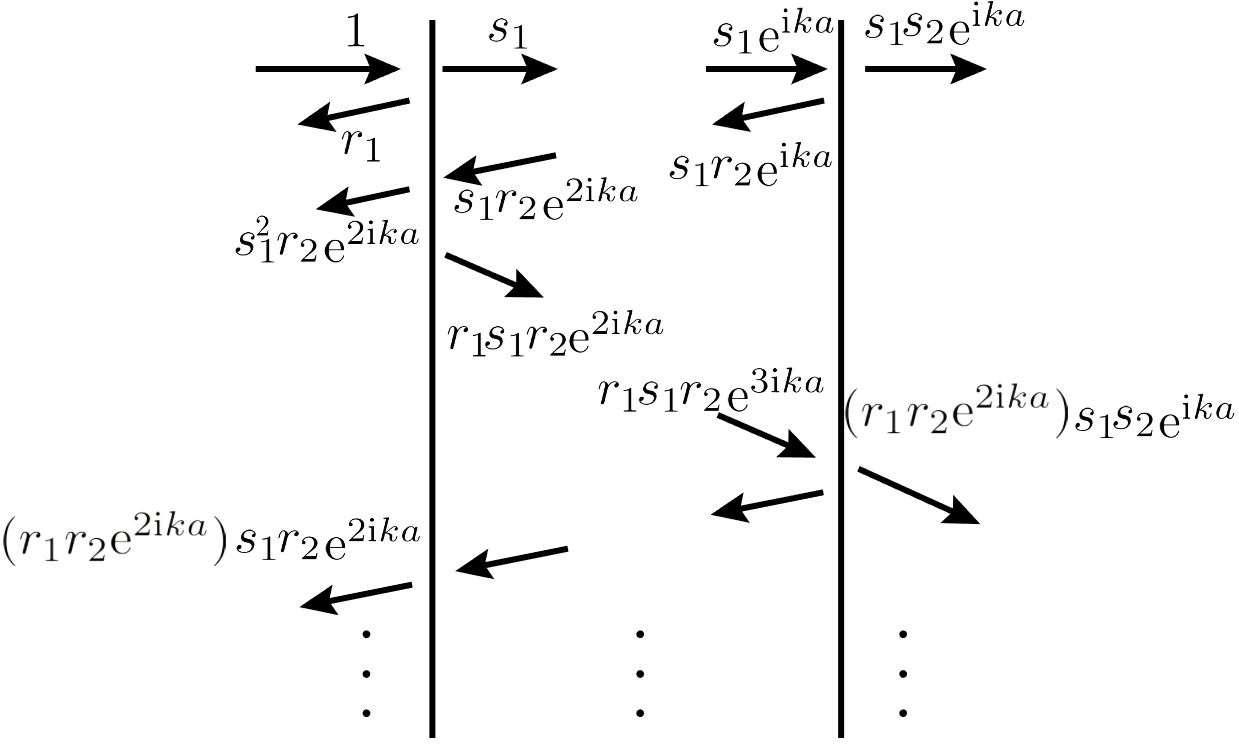
\includegraphics[width=0.5\textwidth]{pic/delta.JPG}
    \label{fig:my_label}
\end{figure}

下面要严格论证的是,将三段区间内的所有波叠加起来,形成的波函数是满足薛定谔方程的;同时因为级数收敛,它是一个合理的解。这是因为在$x=0,\,a$的边界上波函数需满足
\[ \begin{cases}
-\frac{\hbar^2}{2\mu}\qty(\psi'(0^+)-\psi'(0^-))+\gamma_1\psi(0) = 0\\
-\frac{\hbar^2}{2\mu}\qty(\psi'(a^+)-\psi'(a^-))+\gamma_2\psi(a) = 0
\end{cases}\]
而在边界附近可就所有波以“入射、反射、透射”的形式编组,每个组合构成的局域波函数均满足上述方程。由于波函数的叠加性可知道上图即给出一个合理的波函数解。因此,只需统计所有从第1层$\delta$势垒反射回来的波函数即可:
\alg{R &= r_1+s_1^2r_2\ee{2\im ka}\qty(1+r_1r_2\ee{2\im ka}+(r_1r_2\ee{2\im ka})^2+\cdots)\\
&= r_1+s_1^2r_2\ee{2\im ka}\frac{1}{1-r_1r_2\ee{2\im ka}}\\
&= \frac{1}{\im\theta_1 -1}+\frac{-\theta_1^2}{(\im\theta_1 -1)^2}\frac{1}{\im\theta_2 -1}\ee{2\im ka}\frac{(\im\theta_1-1)(\im\theta_2-1)}{(\im\theta_1-1)(\im\theta_2-1)-\ee{2\im ka}}\\
&= \frac{(\im\theta_2-1)+(\im\theta_1+1)\ee{2\im ka}}{(\im\theta_1-1)(\im\theta_2-1)-\ee{2\im ka}}
}
透射系数的计算类似,容易发现结果与《解答》相同。

\item 【另解】

仿照4.26题的方法求解。但此时逐个地对无限层$\delta$势垒写入射波的反射、透射的波函数是不现实的,我们可将所有势垒层看做一个黑箱,且将第2层到$\infty$层势垒视为同样的黑箱。设入射波前振幅为1,经过黑箱后反射系数$u$,透射系数$v$(注意应固定与第一层势垒的距离,相位会随距离变化产生差异),容易绘制出波的传播路径如下。
\begin{figure}[!ht]
    \centering
    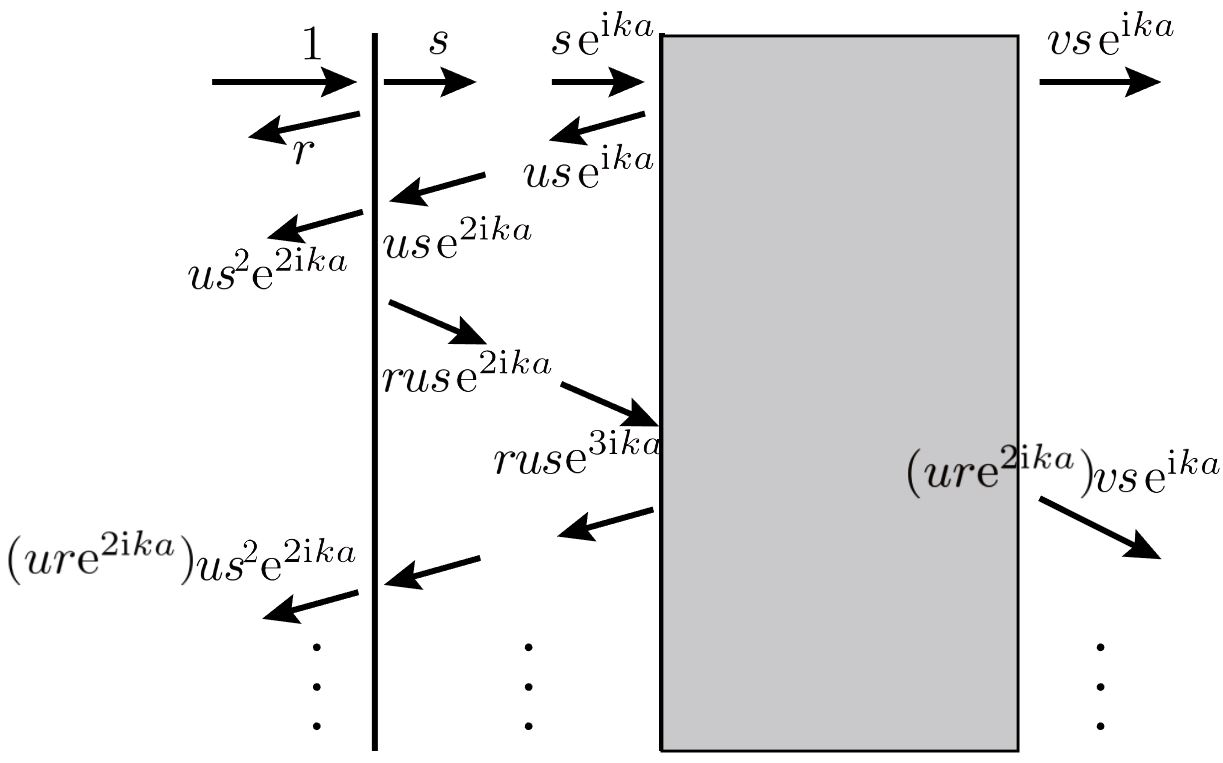
\includegraphics[width=0.5\textwidth]{pic/delta2.JPG}
    \label{fig:my_label}
\end{figure}

经过黑箱的透射波为
\alg{v & = \qty[s\ee{\im ka}\qty(1+ur\ee{2\im ka}+(ur\ee{2\im ka})^2+\cdots)]\,v\,\ee{-\im ka}\\
&= v\,\frac{1+r}{1-ur\ee{2\im ka}}
}
这里用到$s=1+r$. 可得$u\ee{2\im ka}=-1$. 经过黑箱的反射波为
\alg{u &= r+us^2\ee{2\im ka}\qty(1+ur\ee{2\im ka}+(ur\ee{2\im ka})^2+\cdots)\\
&= r+ \frac{u(1+r)^2\ee{2\im ka}}{1-ur\ee{2\im ka}}\\
&= \frac{r+u(1+2r)\ee{2\im ka}}{1-ur\ee{2\im ka}}}
代入$u\ee{2\im ka}=-1$可得$u=-1$,从而$\ee{2\im ka}=1$.

\end{enumerate}

\begin{enumerate}[label=\textbf{4.A\arabic*}, listparindent=\parindent]
    \item (出自《樱井》习题2.12)\textbf{考虑一维谐振子势,若$t=0$时系统处于$\ket{\psi}=\exp(-iAp/\hbar)\ket{0}$态,利用Heisenberg绘景计算$\jkh{x(t)}$和$\jkh{p(t)}$。}\\
    \textbf{解:}首先计算$\zkh{H,\,x}$和$\zkh{H,\,p}$:
    \alg{\zkh{H,\,x}&=\frac{1}{2m}\zkh{p^2,\,x}=-\im\frac{\hbar}{m}p\\
    \zkh{H,\,p}&=\frac{m\omega^2}{2}\zkh{x^2,\,p}=\im\hbar m\omega^2x}
    根据定义,可以写出Heisenberg绘景下坐标算符的表达式:
    \alg{x_\mathrm{H}(t)=\ee{\frac{\im Ht}{\hbar}}x_\mathrm{S}\ee{-\frac{\im Ht}{\hbar}}}
    利用恒等式$\ee{-\alpha\hA}\hB\ee{\alpha\hA}=\sum_{n=0}^\infty\frac{\alpha^n}{n!}(-1)^n(\mathcal{L}_{\hA})^n(\hB)$,可得
    \alg{x_\mathrm{H}(t)&=\sum_{n=0}^\infty\frac{\xkh{\im t/\hbar}^n}{n!}(\mathcal{L}_{H})^n(x_\mathrm{S})\\
    &=\sum_{n=0}^\infty\frac{\xkh{-\omega t}^{2n}}{\xkh{2n}!}x_\mathrm{S}+\frac{1}{m\omega}\sum_{n=0}^\infty\frac{\xkh{-\omega t}^{2n+1}}{\xkh{2n+1}!}p_\mathrm{S}\\
    &=x_\mathrm{S}\cos\omega t+\frac{p_\mathrm{S}}{m\omega}\sin\omega t}
    类似地,可以得到Heisenberg绘景下动量算符的表达式:
    \alg{p_\mathrm{H}(t)=p_\mathrm{S}\cos\omega t-m\omega x_\mathrm{S}\sin\omega t}
    则$t$时刻的$\jkh{x_\mathrm{H}(t)}$为
    \alg{\jkh{x_\mathrm{H}(t)}&=\bra{\psi}x_\mathrm{H}(t)\ket{\psi}\\
    &=\bra{0}\ee{\im\frac{Ap}{\hbar}}x_\mathrm{H}(t)\ee{-\im\frac{Ap}{\hbar}}\ket{0}\\
    &=\bra{0}\xkh{\ee{\im\frac{Ap}{\hbar}}x_\mathrm{S}\ee{-\im\frac{Ap}{\hbar}}\cos\omega t+\frac{1}{m\omega}\ee{\im\frac{Ap}{\hbar}}p_\mathrm{S}\ee{-\im\frac{Ap}{\hbar}}\sin\omega t}\ket{0}\\
    &=\bra{0}\zkh{(x_\mathrm{S}+A)\cos\omega t+\frac{1}{m\omega}p_\mathrm{S}\sin\omega t}\ket{0}\\
    &=A\cos\omega t}
    最后一步可通过将$x$和$p$用升降算符表示得到(易知$\jkh{x}=0$,$\jkh{p}=0$)。类似地,可知
    \alg{\jkh{p_\mathrm{H}(t)}=-Am\omega\sin\omega t}\\
    \textbf{补充:}此系统实际上对应相干态,$t=0$时处在$c$为实数的相干态。下面考察任意相干态的时间演化。考虑相干态
    \alg{\ket{c}=\ee{-\frac{1}{2}\abs{c}^2}\ee{ca\hcj}\ket{0}=\ee{-\frac{1}{2}\abs{c}^2}\sum_0^\infty\frac{c^n}{\sqrt{n!}}\ket{n}}
    由于$\ket{n}$是$H$的本征态,其时间演化只需乘一个相因子,易得
    \alg{\ket{c}(t)&=\ee{-\frac{1}{2}\abs{c}^2}\sum_0^\infty\frac{c^n}{\sqrt{n!}}\ee{-\im\omega t\xkh{n+\frac{1}{2}}}\ket{n}\\
    &=\ee{-\frac{1}{2}\abs{c}^2}\ee{-\frac{1}{2}\im\omega t}\sum_0^\infty\frac{\xkh{c\ee{-\im\omega t}}^n}{\sqrt{n!}}\ket{n}\\
    &=\ee{-\frac{1}{2}\im\omega t}\ket{c\ee{-\im\omega t}}}
    可见相干态在任意$t$时刻仍为相干态。考察$\jkh{x}$和$\jkh{p}$,由于相干态中$\jkh{x}\propto\Re{c}$,$\jkh{p}\propto\Im{c}$,可知$\jkh{x}$和$\jkh{p}$随时间简谐地振荡。这可看作经典谐振子在量子中的对应。
    
    \item(出自《樱井》习题2.18)\textbf{证明一维谐振子势下有}
    \alg{\bra{0}\ee{\im kx}\ket{0}=\exp(-\frac{k^2}{2}\bra{0}x^2\ket{0})}
    \textbf{解:}将$x$用升降算符表示:
    \alg{\ee{\im kx}=\exp(\im k\sqrt{\frac{\hbar}{2m\omega}}\xkh{a+a\hcj})=\exp(\im k\sqrt{\frac{\hbar}{2m\omega}}a\hcj)\exp(\im k\sqrt{\frac{\hbar}{2m\omega}}a)\exp(-\frac{1}{2}k^2\frac{\hbar}{2m\omega})}
    则等式左边可写为:
    \alg{\bra{0}\ee{\im kx}\ket{0}&=\bra{0}\exp(\im k\sqrt{\frac{\hbar}{2m\omega}}a\hcj)\exp(\im k\sqrt{\frac{\hbar}{2m\omega}}a)\exp(-\frac{1}{2}k^2\frac{\hbar}{2m\omega})\ket{0}\\
    &=\exp(-\frac{1}{2}k^2\frac{\hbar}{2m\omega})\bra{0}\exp(\im k\sqrt{\frac{\hbar}{2m\omega}}a\hcj)\ket{0}\\
    &=\exp(-\frac{1}{2}k^2\frac{\hbar}{2m\omega})}
    另一方面,计算$\bra{0}x^2\ket{0}$:
    \alg{\bra{0}x^2\ket{0}=\bra{0}\frac{\hbar}{2m\omega}\xkh{a^2+{a\hcj}^2+aa\hcj+a\hcj a}\ket{0}=\frac{\hbar}{2m\omega}}
    容易看出上式只有$\bra{0}aa\hcj\ket{0}=1$项非0。故有
    \alg{\bra{0}\ee{\im kx}\ket{0}=\exp(-\frac{1}{2}k^2\frac{\hbar}{2m\omega})=\exp(-\frac{1}{2}k^2\bra{0}x^2\ket{0})}
    
    \item(出自《樱井》习题2.16)\textbf{定义关联函数为}
    \alg{C(t)=\jkh{x_\mathrm{H}(t)x_\mathrm{H}(0)}}
    \textbf{计算一维谐振子基态下的$C(t)$。}\\
    利用4.I的结果,有
    \alg{x_\mathrm{H}(t)x_\mathrm{H}(0)=x_\mathrm{S}^2\cos\omega t+\frac{p_\mathrm{S}x_\mathrm{S}}{m\omega}\sin\omega t}
    将$x$和$p$用升降算符表示,有
    \alg{&p\xde x\xde=\im\frac{\hbar}{2}\xkh{-a\xde^2+a\hcj\xde{^2}-1}\\
    &x\xde^2=\frac{\hbar}{2m\omega}\xkh{a\xde{^2}+a\hcj\xde{^2}+a\xde a\hcj\xde+a\hcj\xde a\xde}}
    容易得到
    \alg{&\bra{0}p\xde x\xde\ket{0}=-\im\frac{\hbar}{2}\\
    &\bra{0}x\xde^2\ket{0}=\frac{\hbar}{2m\omega}}
    故
    \alg{C(t)=\frac{\hbar}{2m\omega}\cos\omega t-\im\frac{\hbar}{2m\omega}\sin\omega t=\frac{\hbar}{2m\omega}\ee{-\im\omega t}}

\item (出自程檀生书习题3.13) \textbf{在$xy$平面上运动的质量为$m$,电荷$e$的粒子被置于均匀的磁场中($\vec{B}=B_0\vec{e}_z$),其哈密顿量$\hH$可以表为
\[\hat{H}=\frac{1}{2m}\qty{\hat{p}_x^2+\hat{p}_y^2+eB_0(y\hat{p}_x-x\hat{p}_y)+\frac{1}{4}e^2B_0^2(x^2+y^2)}\]
设\[\hat{b} = \frac{1}{\sqrt{2eB_0 \hbar}}\qty(\frac{1}{2}eB_0x + \im\hat{p}_x+\frac{1}{2}\im eB_0 y-\hat{p}_y),\]
\[\hat{b}^\dagger = \frac{1}{\sqrt{2eB_0 \hbar}}\qty(\frac{1}{2}eB_0x -\im\hat{p}_x-\frac{1}{2}\im eB_0 y-\hat{p}_y),\]
证明: $\hat{H}=\qty(\hat{b}^\dagger\hat{b}+\dfrac{1}{2})\hbar\omega$, 其中$\omega=eB_0/m$.
}

经过计算并利用对易关系,容易得到
\alg{\hat{b}^\dagger\hat{b} &= \frac{1}{2eB_0 \hbar}\qty(\frac{1}{4}e^2B_0^2\qty(x^2+y^2)+\qty(\hat{p}_x^2+\hat{p}_y^2)+\frac{1}{2}\im eB_0\qty[x,\hat{p}_x]+\frac{1}{2}\im eB_0\qty[y,\hat{p}_y]-eB_0x\hat{p}_y+eB_0y\hat{p}_x)\\
&=\frac{1}{2eB_0 \hbar}\qty(\frac{1}{4}e^2B_0^2\qty(x^2+y^2)+\qty(\hat{p}_x^2+\hat{p}_y^2)+eB_0(y\hat{p}_x-x\hat{p}_y)-eB_0\hbar)}
故可以写为$\hat{H}=\qty(\hat{b}^\dagger\hat{b}+\dfrac{1}{2})\hbar\omega$。它具有谐振子的形式,因此能级一定呈等差数列排布。

本题还可继续求解出相应能级的波函数,并发现它是无穷维简并的。(这可以理解为,因为体系是二维的,而写成的谐振子形式却是一维的。)求解细节可参见曾谨言书7.2节。
\end{enumerate}


\newpage
\section{第五章“有心力场及其应用举例”习题解答}
% \begin{center}
%     \Large{\textbf{第五章“有心力场及其应用举例”题目参考答案}}
% \end{center}

\begin{enumerate}[label=\textbf{5.\arabic*}, listparindent=\parindent, leftmargin=-0.5mm]

\setcounter{enumi}{0}

\item 采用球坐标系,分离变量后可得径向方程:
\alg{\frac{1}{r^2}\drv{}{r}\xkh{r^2\drv{R}{r}}+\xkh{\frac{2mE}{\hbar^2}-\frac{l\xkh{l+1}}{r^2}}R=0}
做变量替换,设$u(r)=rR(r)$,得
\alg{\drv{^2u}{r^2}+\xkh{\frac{2mE}{\hbar^2}-\frac{l\xkh{l+1}}{r^2}}u=0}
考虑离原点很远处,$r\to\infty$,方程的第三项$\frac{l\xkh{l+1}}{r^2}u$与第二项相比可以忽略,故方程近似变为
\alg{\drv{^2u}{r^2}+\frac{2mE}{\hbar^2}u=0}
其解为$u(r)=\ee{\pm\im kr}$,$k=\frac{\sqrt{2mE}}{\hbar}$。故波函数可近似表示为
\alg{f(\theta)\frac{u(r)}{r}=f(\theta)\xkh{C_1\frac{\ee{\im kr}}{r}+C_2\frac{\ee{-\im kr}}{r}}}
其中指数上为正号表示发散的球面波,指数上为负号表示会聚的球面波。


\item 实际应将氢原子作为二体问题来处理,设电子与质子的坐标为$\vec{r}_1$, $\vec{r}_2$, 可引进质心坐标$\vec{R}$和相对坐标$\vec{r}$为
\[\vec{r}=\vec{r}_1-\vec{r}_2,\quad \vec{R}=\frac{m_1\vec{r}_1+m_2\vec{r}_2}{m_1+m_2}\]
在量子力学的处理中,将波函数在$\vec{R}$, $\vec{r}$上分离变量$\Psi=\phi(\vec{R})\psi(\vec{r})$, 可得
\alg{-\frac{\hbar^2}{2M}\nabla_R^2\,\phi(\vec{R})& =E_C\phi(\vec{R})\\
\qty(-\frac{\hbar^2}{2\mu}\nabla^2-\frac{e_s^2}{r})\psi(\vec{r})&=E\psi(\vec{r})}
其中$M=m_e+m_p$, $\mu=\frac{m_em_p}{m_e+m_p}$。可见$\phi(\vec{R})$符合自由粒子的运动规律,$\psi(\vec{r})$满足的方程与中心固定的氢原子模型的薛定谔方程相同,因此能级分布规律也相同,只需将原方程中电子质量$m$替换为等效质量$\mu$即可。由此计算的里德堡常量为
\[R = \frac{2\pi^2 \mu e_s^4}{h^3 c} = \frac{m_p}{m_e+m_p}R_\infty\]
$R_\infty$为修正前的里德堡常量。修正后的结果与实验测量符合地很好。

\item (参见《解答》6.1) 

\noindent{\color{red}\textbf{注意:}}第(2)问答案有些问题。Virial定理仅对于定态成立,故不能够将其应用于一个构造的波包上。

\noindent【另解】:在$l$给定时,径向的等效势能为
\[V_r(r) = -\frac{a}{r^s}+\frac{l(l+1)\hbar^2}{2mr^2}\]
由于$0<s<2$,可知$r\rightarrow 0$时$V_r\rightarrow+\infty$;$r\rightarrow +\infty$时$V_r$从负值趋向于0. 这样$V_r$在$r>0$区间内形成一个“无限宽”的势阱。我们可以从薛定谔方程解的特性为出发点:由于一维体系第$i$个能级波函数有$i-1$个节点,我们可证明,在$E\rightarrow 0^-$时,波函数可存在无穷多个节点。

为此,将波函数换元为$\psi(r)=\ee{\phi(r)/\hbar}$,这样$\phi(r)$就包含我们希望研究的波函数“振荡”特性。可推出$\phi(r)$满足的方程
\[\hbar \phi''(r)+[\phi'(r)]^2=2m(V_r(r)-E)\]
考虑$E\rightarrow 0^-$,且$r$很大时,右式主要贡献项为$-\frac{2ma}{r^s}$. 容易猜出一个解,方程的左式主要由$[\phi'(r)]^2$项贡献,即$r\rightarrow+\infty$时$\phi(r)$的趋近行为为
\[\phi'(r)\sim \pm \im\sqrt{2ma}\,r^{-s/2}\]
得到
\[\phi(r)\sim \phi_0(r)\pm\im\frac{2\sqrt{2ma}}{2-s}r^{1-s/2}\]
显然由一维体系的性质$\psi(r)$和$\psi^*(r)$同为满足薛定谔方程的波函数,故可构造实的波函数$\Psi(r)=\frac{1}{2}\qty(\psi(r)+\psi^*(r)) = \ee{\Re\,\phi(r)/\hbar}\cos(\Im\,\phi(r)/\hbar)$,因此
\[\Psi(r)\sim A_0\cos(\frac{2\sqrt{2ma}}{2-s}r^{1-s/2}+\beta_0)\]
因为$0<s<2$,容易发现$\cos$内函数可随着$r$的增加趋于无穷大,故$E\rightarrow 0^-$的波函数可存在无限多个节点,相应地则有无限个能级。

\item (参见《解答》6.3)

\item (参见《解答》6.4)

%6
\item (参见《解答》6.15)

%7
\item 题中的轨道半径应理解为最概然半径,但对于一般的s态与p态无法求出解析结果。下表列出前6个s态与前5个p态的最概然半径、平均半径及相应玻尔轨道半径值作为比较。容易看出,一般情形下有平均半径$>$最概然半径$>$玻尔轨道半径,随$n$的增加而增加,量级为$\order{n^2}$。
\begin{table}[H]
        \centering
        \begin{tabular}{c|c|c|c|c|c|c}
            \hline
            $n$ & 1 & 2 & 3 & 4 & 5 & 6 \\\hline
            玻尔轨道半径 $/a_0 $ & 1.0000 & 4.0000 & 9.0000 & 16.0000 & 25.0000 & 36.0000 \\
            最概然半径 $/a_0 $ &1.0000 &  5.23607 & 11.4772 &  19.6257 &  29.7159 & 41.7737 \\
            平均半径 $/a_0 $ & 1.5000 & 6.0000 & 13.5000 &  24.0000 & 37.5000 & 54.0000\\\hline
        \end{tabular}
        \caption{5.7题的结果:前6个s态的各个半径对照}
        \label{tab:my_label}
    \end{table}
\begin{table}[H]
        \centering
        \begin{tabular}{c|c|c|c|c|c}
            \hline
            $n$ &  2 & 3 & 4 & 5 & 6 \\\hline
            玻尔轨道半径 $/a_0 $ & 4.0000 & 9.0000 & 16.0000 & 25.0000 & 36.0000 \\
            最概然半径 $/a_0 $ & 4.0000 & 10.772 & 19.1132 & 29.3106 & 41.4378 \\
            平均半径 $/a_0 $ & 4.0000 &  11.500 &  22.0000 & 35.500 & 52.0000\\\hline
        \end{tabular}
        \caption{5.7题的结果:前5个l态的各个半径对照}
        \label{tab:my_label}
    \end{table}

%8
\item 
\begin{enumerate}[label=(\arabic*)]
    \item 根据玻尔模型,可以得出玻尔半径为
    \alg{r_n=\frac{4\pi\varepsilon_0\hbar^2}{e^2\mu}\frac{n^2}{Z}}
    以及速度
    \alg{v_n=\frac{e^2}{4\pi\varepsilon_0\hbar}\frac{Z}{n}}
    计算出结果列于表3。
    \begin{table}[h]
        \centering
        \begin{tabular}{c|c|c|c}
            \hline
            & H & He$^+$ & Li$^{++}$ \\
            \hline
            $r_1$/m & $5.3\et{-11}$ & $2.6\et{-11}$ & $1.8\et{-11}$ \\
            $r_2$/m & $2.1\et{-10}$ & $1.1\et{-10}$ & $7.1\et{-11}$ \\
            \hline
            $v_1$/(m$\cdot$s$\inv$) & $2.2\et{6}$ & $4.4\et{6}$ & $6.6\et{6}$ \\
            $v_2$/(m$\cdot$s$\inv$) & $1.1\et{6}$ & $2.2\et{6}$ & $3.3\et{6}$ \\
            \hline
            $E_1$/eV & 13.6 & 54.4 & 123 \\
            \hline
            $\Delta E$/eV & 10.2 & 40.8 & 91.9 \\
            $\lambda$/nm & 122 & 30.4 & 13.5 \\
            \hline
        \end{tabular}
        \caption{5.8\,题的结果}
        \label{tab:my_label}
    \end{table}
    
    \item 根据玻尔模型,可得类氢离子能级:
    \alg{E_n=-\frac{e^4\mu}{32\pi^2\varepsilon_0^2\hbar^2}\frac{Z^2}{n^2}}
    电子的结合能即为$E_1$,计算结果列于表3。
    
    \item 由基态到第一激发态的激发能为
    \alg{\Delta E=E_2-E_1=\frac{3e^4\mu}{128\pi^2\varepsilon_0^2\hbar^2}Z^2}
    由第一激发态退激到基态时所发光的波长为
    \alg{\lambda=\frac{hc}{\Delta E}}
    计算结果列于表3。
\end{enumerate}

%9
\item 由Virial定理,在库仑势$V(r)\propto r\inv$下,有$2\jkh{T}_n=-\jkh{V}_n$。又由于$\jkh{T}_n+\jkh{V}_n=E_n=-\frac{e^4\mu}{32\pi^2\varepsilon_0^2\hbar^2n^2}$,可得
\alg{\jkh{T}_n&=-E_n=\frac{e^4\mu}{32\pi^2\varepsilon_0^2\hbar^2n^2}\propto E_n\\
\jkh{V}_n&=2E_n=-\frac{e^4\mu}{16\pi^2\varepsilon_0^2\hbar^2n^2}\propto E_n}
角速度可以由玻尔模型的速度与轨道半径定义:
\alg{\omega_n=\frac{v_n}{r_n}=\frac{e^4\mu}{16\pi^2\varepsilon_0^2\hbar^3}n^{-3}\propto E_n^{\frac{3}{2}}}

%10
\item 类氢原子的径向波函数$R_{nl}(r)$有
\alg{R_{nl}(r)\propto\ee{-\frac{x}{2}}x^lL_{n-l-1}^{2l+1}\xkh{{x}}}
其中$x=\frac{\mu Ze^2}{2n\pi\varepsilon_0\hbar^2}r$。角向波函数为球谐函数,
\alg{Y_{lm}(\theta,\,\phi)\propto P_{lm}(\cos\theta)\ee{\im m\phi}}
通过繁而不难的计算容易得到各情况下的节点,结果列于表4。
\begin{table}[h]
    \centering
    \begin{tabular}{ccc|c|c}
    \hline
        $n$ & $l$ & $m$ & 径向节点 & 角向节点 \\
        \hline
        1 & 0 & 0 & 无 & 无 \\
        \hline
        2 & 0 & 0 & $x=2$ & 无 \\
        2 & 1 & 0 & $x=0$ & $\theta=\frac{\pi}{2}$ \\
        2 & 1 & $\pm1$ & $x=0$ & $\theta=0,\,\pi$ \\
        \hline
        3 & 0 & 0 & $x=3\pm\sqrt{3}$ & 无 \\
        3 & 1 & 0 & $x=0,\,4$ & $\theta=\frac{\pi}{2}$ \\
        3 & 1 & $\pm1$ & $x=0,\,4$ & $\theta=0,\,\pi$ \\
        \hline
        3 & 2 & 0 & $x=0$ & $\theta=\arccos(\pm\frac{1}{\sqrt{3}})$ \\
        3 & 2 & $\pm1$ & $x=0$ & $\theta=0,\,\frac{\pi}{2},\,\pi$ \\
        3 & 2 & $\pm2$ & $x=0$ & $\theta=0,\,\pi$\\
        \hline
    \end{tabular}
    \caption{5.10题的结果}
    \label{tab:my_label}
\end{table}

%11
\item 平均半径$\bar{r}$的求解请见5.14题,各量子态$(n,\,l)$按照半径由小到大的排列顺序为:

\begin{small}
\noindent(1,0), (2,1), (2,0), (3,2), (3,1), (3,0), (4,3), (4,2), (4,1), (4,0), (5,4), (5,3), (5,2), (5,1), (5,0), (6,5), (6,4), (6,3), (6,2), (7,6), (6,1), (6,0), (7,5), (7,4), (7,3), (8,7), (7,2), (7,1), (7,0), (8,6), (8,5), (9,8), (8,4), (8,3), (8,2), (9,7), (8,1), (8,0), (9,6), (10,9), (9,5), (9,4), (10,8), (9,3), (9,2), (9,1), (9,0), (10,7), (11,10), (10,6), (10,5), (11,9), (10,4), (10,3), (11,8), (10,2), (10,1), (10,0), (12,11), (11,7), (11,6), (12,10), (11,5), (12,9), (11,4), (13,12), (11,3), (11,2), (12,8), (11,1), (11,0), (13,11), (12,7), (12,6), (13,10), (12,5), (14,13), (12,4), (13,9), (12,3), (12,2), (12,1), (14,12), (12,0), (13,8), (13,7), (14,11), (15,14), (13,6), (13,5), (14,10), (13,4), (15,13), (13,3), (14,9), (13,2), (13,1), (13,0), (14,8), (15,12), (16,15), (14,7), (15,11), (14,6), (14,5), (16,14), (15,10), (14,4), (14,3), (14,2), (15,9), (14,1), (16,13), (14,0), (17,16), (15,8), (16,12), (15,7), (17,15), (15,6), (16,11), (15,5), (15,4), (17,14), (16,10), (15,3), (18,17), (15,2), (15,1), (15,0), (16,9), (17,13), (16,8), (18,16), (17,12), (16,7), (16,6), (18,15), (17,11), (16,5), (19,18), (16,4), (16,3), (17,10), (16,2), (18,14), (16,1), (16,0), (17,9), (19,17), (18,13), (17,8), (17,7), (19,16), (18,12), (20,19), (17,6), (17,5), (18,11), (19,15), (17,4), (17,3), (20,18), (17,2), (18,10), (17,1), (17,0), (19,14), (18,9), (20,17), (18,8), (19,13), (18,7), (19,12), (20,16), (18,6), (18,5), (19,11), (18,4), (18,3), (20,15), (18,2), (18,1), (18,0), (19,10), (20,14), (19,9), (19,8), (20,13), (19,7), (19,6), (20,12), (19,5), (19,4), (20,11), (19,3), (19,2), (19,1), (19,0), (20,10), (20,9), (20,8), (20,7), (20,6), (20,5), (20,4), (20,3), (20,2), (20,1), (20,0).
\end{small}

关于概率密度分布的讨论:
\begin{enumerate}
    \item 当角量子数$l$给定时,本征态的能量随着$n$的增加而增加。由于远离原子核的电子总能量更高,因此电子的概率密度倾向于更加远离中心。同时,$l$给定时径向的等效势能完全确定,根据薛定谔方程的特性,随着$n$的增加,径向波函数的节点个数按照0, 1, 2$\cdots$的顺序逐个增加。
    \item 当主量子数$n$给定时,随着$l$的增大,电子的概率密度分布更加接近中心。这是由于类氢离子的$n$相同的所有能级都是简并的,伴随着$l$的增大,切向方向的动能有所增加,因此径向方向的能量会减小,使得电子更靠近原子核。
\end{enumerate}

%12
\item 电流可以通过玻尔模型中的速度和半径来定义:
\alg{I_n=\frac{v_ne}{2\pi r_n}=\frac{e^5\mu}{32\pi^3\varepsilon_0^2\hbar^3n^3}}
磁矩则可以利用角动量来定义:
\alg{m_n=\frac{L_ne}{2\mu}=\frac{n\hbar e}{2\mu}}
计算结果列于表5中。
\begin{table}[h]
    \centering
    \begin{tabular}{c|c|c}
    \hline
        $n$ & $I_n$/A & $m_n$/(A$\cdot$m$^2$) \\
        \hline
        1 & $1.05\et{-3}$ & $9.3\et{-24}$ \\
        2 & $1.3\et{-4}$ & $1.9\et{-23}$ \\
        3 & $3.9\et{-5}$ & $2.8\et{-23}$ \\
        \hline
    \end{tabular}
    \caption{5.12题的结果}
    \label{tab:my_label}
\end{table}

\item (参见《解答》6.14)

\item (参见《解答》6.12)

\noindent{\color{red}\textbf{注意:}}《解答》中给出的$\jkh{r^{-4}}$表达式错误,请以曾谨言书上答案为准。
\[\jkh{r^{-4}} = \frac{Z^4}{a^4}\frac{3n^2-l(l+1)}{2n^5l(l-\frac{1}{2})l(l+\frac{1}{2})(l+1)(l+\frac{3}{2})}\]

\item (参见《解答》6.16)

%16
\item 
\begin{enumerate}[label=(\arabic*)]
    \item 基态的电子偶素中正负电子的距离可用第一玻尔轨道半径表示。对电子偶素,应取等效质量$\mu = \frac{m_e^2}{m_e+m_e} = \frac{m_e}{2}$,故玻尔半径为$a_0 = \frac{\hbar^2}{\mu e_s^2} = 1.06\ai$.

    \item 基态电子的电离能为$E_{\text{电离}}=-E_1 = \frac{\mu e_s^4}{2\hbar^2} = \frac{e_s^2}{2 a_0} = 6.08\eV$,从基态到第一激发态的激发能为$\Delta E = E_2-E_1 = -\frac{3}{4}E_1 = 5.10\eV$.
    
    \item 从第一激发态退到基态发出波长为$\lambda = \frac{hc}{\Delta E} = 243\nm$. 
\end{enumerate}


\item 
\begin{enumerate}[label=(\arabic*)]
    \item 首先求出$\mu^-$粒子的等效质量为$\mu = \frac{m_\mu m_p}{m_\mu+m_p} = 186.0 \,m_
    e$. 里德堡常量为$R = \frac{2\pi^2 \mu e_s^4}{h^3 c} = 2.04\ten{9}\;\mathrm{m^{-1}}$.
    
    \item 第一玻尔轨道半径为$a_0 = \frac{\hbar^2}{\mu e_s^2} = 0.284\;\mathrm{pm}$.
    
    \item 最低能量为$E_1 = -\frac{e_s^2}{2 a_0} = -2.53\keV$.
    
    \item 光谱莱曼系中的最短波长对应于最大能量,故应为$\infty$能级跃迁到基态的光子的波长,为$\lambda = \frac{hc}{-E_1} = 0.490\nm$.
\end{enumerate}


\noindent{\color{red}\textbf{注意:}}第(4)问不少同学想成第一激发态到跃迁到基态的光子,还需更加谨慎。


\item
\begin{enumerate}[label=(\arabic*)]
    \item 首先求出$\pi^-$介子的等效质量为$\mu = \frac{m_\pi m_p}{m_\pi+m_p} = 235.4\,m_e$. 里德堡常量为$R = \frac{2\pi^2 \mu e_s^4}{h^3 c} = 2.58\ten{9}\;\mathrm{m^{-1}}$.
    \item 能谱为$E_n = \frac{\mu e_s^4}{2\hbar^2}E_1 = -\frac{3.20}{n^2}\keV$.
    \item 第$n$玻尔轨道半径为$r_n = n^2a_0$,且玻尔半径$a_0 = \frac{\hbar^2}{\mu e_s^2} = 0.225\;\mathrm{pm}$,计算得到第一、第二、第三、第四、第五玻尔轨道半径分别为$0.225\;\mathrm{pm}$,$0.899\;\mathrm{pm}$,$2.02\;\mathrm{pm}$,$3.60\;\mathrm{pm}$,$5.62\;\mathrm{pm}$.
\end{enumerate}

\item 本题的势能函数无法就$l\geq 1$的态进行解析求解,感兴趣的同学可尝试使用程序数值求解后与题中给出的观测值进行对照。

\item (参见《解答》6.18)

%21
\item (参见《解答》6.19)

\item (参见《解答》6.20)

\item (参见《解答》6.21)

\item (参见《解答》6.23)

\item (参见《解答》6.22)

%26
\item (参见《解答》6.25)

\noindent{\color{red}\textbf{讨论:}}不少同学没有论述清楚为什么对势场$V(\vec{x})>V_c(\vec{x})$,各自相应的第$i$能级始终有$E_i>E_{ci}$。《解答》中仅说根据HF定理可知,但这里显然应补充更多细节。

构造$V_c(r) = -V_0 a/r$,则$V(\vec{x})>V_c(\vec{x})$在任意坐标点$\vec{x}$处成立。可以构造新的势能$V_{\lambda}(\vec{x}) = (1-\lambda) V_c(\vec{x}) + \lambda V(\vec{x})$随参数$\lambda$变化,$\lambda\in[0,\,1]$, 且$\lambda=0$和$1$时势能分别取$V_c(\vec{x})$和$V(\vec{x})$. 显然,对任意$\vec{x}$有
\[\pdv{V_\lambda(\vec{x})}{\lambda} = V(\vec{x})-V_c(\vec{x})>0.\]
于是,对于任意波函数$\Psi(\vec{x})$都有
\[\left\langle \pdv{H_\lambda}{\lambda}\right\rangle = \left\langle \pdv{V_\lambda}{\lambda}\right\rangle = \iiint_\Omega \Psi^*(\vec{x})\qty(V(\vec{x})-V_c(\vec{x}))\Psi(\vec{x})\dd[3]{\vec{x}}>0.\]
根据HF定理,对$H_\lambda$的第$i$个本征态及其本征值$E_{i,\lambda}$,有
\[\left\langle \pdv{H_\lambda}{\lambda}\right\rangle = \pdv{E_{i,\lambda}}{\lambda},\]
因此$\pdv*{E_{i,\lambda}}{\lambda}>0$,即$H_{\lambda}$的第$i$个本征值$E_{i,\lambda}$在$\lambda\in [0,\,1]$上为增函数。可知$\eval{E_{i,\lambda}}_{\lambda=1}>\eval{E_{i,\lambda}}_{\lambda=0}$, 即$E_i>E_{ci} $证毕。

\item 束缚态波函数分离变量为$\psi(r,\theta,\varphi)=R_n(r)\Y_{lm}(\theta,\phi)$. $R_n(r)$满足的径向薛定谔方程:
\[\frac{1}{r}\dv[2]{r}\qty(rR_n(r)) + \qty[\frac{2m}{\hbar^2}(E-V(r))-\frac{l(l+1)}{r^2}]R_n(r) = 0.\]
记$R(r)=\chi(r)/r$,$\chi_n(r)$满足
\[\dv[2]{\chi}{r}+\qty[\frac{2m}{\hbar^2}(E-V(r))-\frac{l(l+1)}{r^2}]\chi = 0\]
考虑径向波函数的等效势为$V'=V+\frac{l(l+1)\hbar^2}{2mr^2}$,根据HF定理,将$l$升级为连续变量后选定其为参量,对径向量子数$n$的径向本征波函数,有
\[\pdv{E}{l}=\jkh{\pdv{H}{l}} = (2l+1)\frac{\hbar^2}{2m}\jkh{\frac{1}{r^2}}>0,\] 可推知径向量子数相同的能级,能量随$l$的增大而增大,故本题需求解的基态波函数一定为$l=0$时径向波函数的基态。题目的势能函数为
\[V(r) = \begin{cases}0, & R_1<r<R_2\\
+\infty, &\text{其他}
\end{cases}\]
因此$l=0$, $r\in(R_1,\,R_2)$区间内$\chi(r)$方程退化为谐振子方程,通解为
\[\chi(r) = A\sin(kr-\phi),\quad k=\frac{\sqrt{2mE}}{\hbar}\]
边界条件$\chi(R_1)=0$, $\chi(R_2)=0$。可解得$k(R_2-R_1)=n_r\pi$, $kR_1-\phi=n_r'\pi$。考虑到$n_r'$的取值只影响波函数的正负号,归一化后无影响,故取$n_r'=0$, 即$\phi=kR_1$。径向波函数写作
\[R_n(r) = \frac{\chi_n(r)}{r} = \frac{1}{r}\sin\frac{n\pi (r-R_1)}{R_2-R_1}\]
对径向归一化:
\[\int_0^{+\infty} \abs{R(r)}^2r^2\dd{r} = 1\]
得$A=\sqrt{\frac{2}{R_2-R_1}}$。又知
角向波函数为$\Y_{00}(\theta,\varphi)=\frac{1}{\sqrt{4\pi}}$,故基态波函数为
\[\phi_{100}=\sqrt{\frac{1}{2\pi(R_2-R_1)}}\,\frac{1}{r}\sin\frac{n\pi(r-R_1)}{R_2-R_1},\]
本征能量为
\[E_{100} = \frac{\pi^2\hbar^2}{2m(R_2-R_1)^2}\]

\noindent{\color{red}\textbf{说明:}}不少同学没有进行归一化或归一化错误,还请留意。
\item (5.28--30题及5.31 (4)问略,不要求)

\setcounter{enumi}{30}
\item (参见《解答》6.2)

\noindent{\color{red}\textbf{讨论:}} 我们大致说明一下第(3)问用经典的相空间估算量子态数目的合理性。有一种近似求解大量子数薛定谔方程的方法称为WKB近似,它将波函数的振幅部分与相位部分以$\hbar$为小量展开,逐级进行求解。这种方法能反映出量子力学到经典哈密顿力学的过渡,由它是可以推导出本题使用的相空间体积公式的,虽然具体过程十分复杂。

另外值得补充的是,在一维体系下,相空间体积变为$p-x$构成的相平面面积。(具体来说,是所有满足经典条件$E>V_0$的粒子运动状态在相平面上的点构成的面积。)而面积的计算可写作$\oint p\dd{x}=nh$, 可见这正是旧量子论中的索末菲量子化条件。


\item 题中给出的势能是中子与质子的相互作用势$U$随它们之间距离$r$的关系。可引进质心坐标$\vec{R}$与相对坐标$\vec{r}$换元,即
\[\vec{r}=\vec{r}_1-\vec{r}_2,\quad \vec{R}=\frac{m_1\vec{r}_1+m_2\vec{r}_2}{m_1+m_2}\]
分离变量后可知$\vec{R}$符合自由粒子薛定谔方程,关于$\vec{r}$的方程为
\[\qty(-\frac{\hbar^2}{2\mu}\laplacian + U(\vec{r}))\psi(\vec{r})=E\psi(\vec{r})\]
正是中心势场下三维球方势阱的模型。由5.31题的结果,结合等效质量$\mu = \frac{m_N}{2}$可知出现第一个s态波函数的条件为
\[U_0 = \frac{\pi^2\hbar^2}{4m_N r_0^2}.\]


\item 核子数$Z$的类氢例子基态波函数为
\[\varPsi_Z(\vec{r}) = \frac{2}{\sqrt{4\pi}}\qty(\frac{Z}{a_0})^{3/2}\ee{-Zr/a_0}\]
其中$a_0$为玻尔半径。本题需求解$\varPsi_Z(\vec{r})$态到$\varPsi_{Z+1}(\vec{r})$态的跃迁概率。先求解跃迁振幅为
\alg{\braket{\varPsi_{Z+1}}{\varPsi_Z} &= \intzif \frac{4Z^{3/2}(Z+1)^{3/2}}{a_0^3}\ee{-(2Z+1)r/a_0}\,r^2\dd{r}\int_0^{\pi}\frac{1}{4\pi}\sin^2{\theta}\dd{\theta}\int_0^{2\pi}\dd{\phi}\\
&= \frac{Z^{3/2}(Z+1)^{3/2}}{(Z+\frac{1}{2})^3},}
因此跃迁概率为
\[P = \abs{\braket{\varPsi_{Z+1}}{\varPsi_Z}}^2 = \frac{Z^3(Z+1)^3}{(Z+\frac{1}{2})^6}.\]

\noindent{\color{red}\textbf{注意:}}跃迁概率是跃迁振幅的模方,请大家留意。

\end{enumerate}


\newpage
\section{第三、四、五章小测补充题解答}
% \begin{center}
%     \Large{\textbf{第三、四、五章小测解答}}
% \end{center}

角动量算符的对易关系:$\zkh{q_i,\,l_j}=\ihb\eijk q_k\quad\zkh{\vec{q}^2,\,l_i}=0$,其中$q$可以代表$r$,$p$或$l$。

常用恒等式:

$\ee{\alpha\hA}\hB\ee{-\alpha\hA}=\sum_{n=0}^\infty\frac{\alpha^n}{n!}(\mathcal{L}_{\hA})^n(\hB)$,其中$\mathcal{L}_{\hA}(\hX)=\zkh{\hA,\,\hX}$

$\ee{\hA+\hB}=\ee{\hA}\ee{\hB}\ee{-\frac{1}{2}\hC}$,其中$\hC=\zkh{\hA,\,\hB}$,且$\hC$与$\hA$和$\hB$均对易

\begin{enumerate}[label=\textbf{3.\Alph*}, listparindent=\parindent, leftmargin=-0.5mm]

\setcounter{enumi}{5}
\item \emph{题目:定义产生消灭算符
\alg{\ha^\dagger = \sqrt{\frac{1}{2}}\qty(\sqrt{\frac{m\omega}{\hbar}}\hat{x} - \im\sqrt{\frac{1}{m\hbar\omega}}\hat{p})\\
\ha = \sqrt{\frac{1}{2}}\qty(\sqrt{\frac{m\omega}{\hbar}}\hat{x}+ \im\sqrt{\frac{1}{m\hbar\omega}}\hat{p})}
证明:
\begin{enumerate}
    \item 相干态
    \alg{\ket{c}=\ee{c\ha\hcj-c\cj \ha}\ket{0}}是$\ha$的归一化的本征态,本征值为$c$,其中$c$是$\ha^\dagger\ha$的本征态,本征值为$0$.
    \item 相干态$\ket{c}$中坐标和动量满足
    \alg{\sqrt{\jkh{\Delta x^2}\jkh{\Delta p^2}}=\frac{\hbar}{2}.}
\end{enumerate}
}
\noindent【解答】

\begin{enumerate}
    \item 由于$\zkh{\ha,\,\ha\hcj}=1$为常数,可利用恒等式$\ee{\hA+\hB}=\ee{\hA}\ee{\hB}\ee{-\frac{1}{2}\hC}$得到
    \alg{\ee{c\ha\hcj-c\cj \ha}=\ee{-\frac{\abs{c}^2}{2}}\ee{ca\hcj}\ee{-c\cj a}}
    又由于$\ha\ket{0}=0$,可知$\ee{-c\cj \ha}\ket{0}=\ket{0}$,因此
    \alg{\ket{c}&=\ee{c\ha\hcj-c\cj \ha}\\
    &=\ee{-\frac{\abs{c}^2}{2}}\ee{c\ha\hcj}\ket{0}\\
    &=\ee{-\frac{\abs{c}^2}{2}}\sum_{n=0}^\infty\frac{c^n}{\sqrt{n!}}\ket{n}}
    容易看出$\ket{c}$是归一化的,因为
    \alg{\bra{c}\ket{c}=\ee{-\abs{c}^2}\sum_{n=0}^\infty\frac{\abs{c^2}^n}{n!}=\ee{-\abs{c^2}}\ee{\abs{c^2}}=1}
    这里用到了$\ket{n}$这组基正交归一的性质。下面证明$\ket{c}$是$\ha$的本征态:
    \alg{\ha\ket{c}&=\ee{-\frac{\abs{c}^2}{2}}\sum_{n=0}^\infty\frac{c^{n}}{\sqrt{n!}}\sqrt{n}\ket{n-1}\\
    &=\ee{-\frac{\abs{c}^2}{2}}\sum_{n=1}^\infty c\frac{c^{n-1}}{\sqrt{(n-1)!}}\ket{n-1}\\
    &=c\ket{c}}
    可见$\ket{c}$是$\ha$的本征态,本征值是$c$.
    
    \item 首先将$x$和$p$用产生消灭算符表示:
    \alg{&x=\sqrt{\frac{\hbar}{2m\omega}}\xkh{\ha\hcj+\ha}\\
    &p=\im\sqrt{\frac{\hbar m\omega}{2}}\xkh{\ha\hcj-\ha}\\
    &x^2=\frac{\hbar}{2m\omega}\xkh{2\ha\hcj \ha+1+\ha\hcjsq+\ha^2}\\
    &p^2=\frac{1}{2}\hbar m\omega\xkh{2\ha\hcj \ha+1-\ha\hcjsq-a^2}}
    由于$\ket{c}$是$a$的本征态,容易得到$\jkh{\ha}=c$,$\jkh{\ha^2}=c^2$,以及
    \alg{&\jkh{\ha\hcj}=\xkh{\ket{c},\,\ha\hcj\ket{c}}=\xkh{\ha\ket{c},\,\ket{c}}=c\cj\xkh{\ket{c},\,\ket{c}}=c\cj\\
    &\jkh{\ha\hcj \ha}=\xkh{\ket{c},\,\ha\hcj \ha\ket{c}}=\xkh{\ha\ket{c},\,\ha\ket{c}}=c\cj c\xkh{\ket{c},\,\ket{c}}=\abs{c}^2\\
    &\jkh{\ha\hcjsq}={c\cj}^2}
    其中$\xkh{\ket{i},\,\ket{j}}$表示内积。容易看出
    \alg{&\jkh{x}=\sqrt{\frac{\hbar}{2m\omega}}\xkh{c+c\cj}\\
    &\jkh{p}=\im\sqrt{\frac{\hbar m\omega}{2}}\xkh{c\cj-c}\\
    &\jkh{x^2}=\frac{\hbar}{2m\omega}\xkh{2\abs{c}^2+1+c^2+{c\cj}^2}\\
    &\jkh{p^2}=\frac{\hbar m\omega}{2}\xkh{2\abs{c}^2+1-c^2-{c\cj}^2}}
    由此可得
    \alg{\Delta x\Delta p=\sqrt{\xkh{\jkh{x^2}-\jkh{x}^2}\xkh{\jkh{p^2}-\jkh{p}^2}}=\frac{\hbar}{2}}
    
\end{enumerate}
\end{enumerate}


\begin{enumerate}[label=\textbf{4.\Alph*}, listparindent=\parindent, leftmargin=-0.5mm]
\setcounter{enumi}{2}
\item \emph{题目:曾书3.26题,将势能函数改为
\alg{V(x)=\begin{cases}\gamma\,\delta(x), &x< a\\\infty,&x\geq a\end{cases}}
其中$a>0$.}

\noindent【解法一】

采用常规方法计算。首先分析出波函数$\psi(a)=0$, 可分三个区间设波函数为
\alg{\psi(x)=\begin{cases}
\ee{\im k x} + r\ee{-\im k x},& x<0\\
A\sin k(x-a), &0\leq x< a\\
0,& x\geq a
\end{cases}}
待定参量为$r$和$A$。
根据$x=0,\,a$的边条件有
\alg{&1+r = -A\sin ka\\
&\im k(1-r) + \frac{2m\gamma}{\hbar^2}(1+r)=k A\cos ka}
按照之前单$\delta$势无量纲化的方案,设$\theta = \frac{k\hbar^2}{m\gamma}$,
则第二个等式化简为
\[\im\theta (1-r)+2(1+r)=\theta A\cos ka\]
与第一个等式相除,可以化简得到
\[r = \frac{-\im\theta-2-\theta\cot ka}{-\im\theta+2+\theta\cot ka}
= \frac{-\theta \cos ka + (-2-\im\theta)\sin ka}{\theta \cos ka + (2-\im\theta)\sin ka}
= \frac{\ee{-\im ka}+(-1-\im\theta)\,\ee{\im ka}}{(-1+\im\theta)\,\ee{-\im ka}+\ee{\im ka}}\]
上面三种结果是等价表述。显然地,反射系数为$R=\abs{r}^2=1$,透射系数$T=1-R=0$。不存在完全透射即$T=1$的情况。

\noindent{\color{red}\textbf{说明:}}本题的透射系数是针对整个体系而言的,即应考虑$x>a$区域内透射波的情况(显然无透射波存在)。部分同学考虑了经过$\delta(x)$的“透射系数”,但这样其实没有较好的定义,因为$x<0$和$0<x<a$区间内都含有沿两个方向传递的波的成分。抱歉本题没说清楚,大家只要正确计算出上面的$r$就算对了。

\noindent【解法二】

可参考4.26、4.27作业解答里给出的特殊解法。考虑入射波$\ee{\im kx}$,让该波在$\delta$势和墙壁之间无限次反射、透射,可得全空间波的分布,请同学们自己画示意图。需要注意,这里的墙壁会给波带来“半波损失”的效果,即入射墙壁的波前振幅为$\tilde{A}$的话,反射波前振幅应为$-\tilde{A}$,这样才能使二者在墙壁处叠加为0.

由4.26知单$\delta$势对波的反射与透射有$r_0=\frac{1}{\im\theta-1}$, $s_0=\frac{\im\theta}{\im\theta-1}$,将所有$x<0$区域沿$-x$方向传播的波的波前叠加,得到
\alg{r &= r_0-s_0^2\ee{2\im ka}\qty(1-r_0\ee{2\im ka}+(-r_0\ee{2\im ka})^2+\cdots)\\
&= r_0 -\frac{s_0^2\ee{2\im ka}}{1+r_0\ee{2\im ka}} = \frac{r_0-(1+2r_0)\,\ee{2\im ka}}{1+r_0\ee{2\im ka}}
= \frac{\ee{-\im ka}-(1+\im\theta)\,\ee{\im ka}}{(-1+\im\theta)\,\ee{-\im ka}+\ee{\im ka}}}
与法一结果相同。
\end{enumerate}

\begin{enumerate}[label=\textbf{5.\Alph*}, listparindent=\parindent, leftmargin=-0.5mm]
\setcounter{enumi}{1}
\item \emph{作业5.20题加分小问:计算能量满足$E<E_0$ ($E_0$很大)系统的束缚态能级数量,再从相空间的角度计算束缚态能级数量,二者比较结果。(注:$z$向动能不计入总能量)}

\noindent【解答】

本题讨论二维谐振子模型,能级为
\[E = (n_1+n_2+1)\hbar \omega\]
对$E<E_0$的能级,要求$n_1+n_2+1<\frac{E_0}{\hbar \omega}$,其中$\frac{E_0}{\hbar \omega}\gg 1$。$n_1,\,n_2$取非负整数,这样的能级数量约为$N = \frac{1}{2}\qty(\frac{E_0}{\hbar\omega})^2$个。

再从相空间考虑,设二维谐振子
\[H = \frac{p_x^2}{2m}+\frac{p_y^2}{2m}+\frac{1}{2}m\omega^2 x^2+\frac{1}{2}m\omega^2 y^2,\]
相空间为$(x,\,y,\,p_x,\,p_y)$构成的四维空间。相空间上满足$H<E_0$的点所构成区域(即经典可达到的点构成的区域)应为四维椭球。需要知道半径为$R$的四维球的超体积公式为
\[V = \frac{1}{2}\pi^2R^4,\quad(\text{$N$维球超体积公式为$V = \frac{\pi^\frac{N}{2}}{\Gamma(1+\frac{N}{2})}R^N$})\]
则四维椭球的超体积为
\[V = \frac{1}{2}\pi^2\cdot\sqrt{2mE_0}\cdot \sqrt{2mE_0} \cdot \sqrt{\frac{2E_0}{m\omega^2}} \cdot \sqrt{\frac{2E_0}{m\omega^2}} = \frac{2\pi^2E_0^2}{\omega^2}\]
若量子态个数为$n$,应当有$V \approx nh$,因此
\[n = \frac{2\pi^2E_0^2}{h^2\omega^2 } = \frac{E_0^2}{2\hbar^2\omega^2}\]
与直接求解能级个数的结果相同。

\item \emph{题目:
一电子质量$\mu$,电荷$-e$被限制在$R_1<\rho<R_2$, $0<z<L$的中空圆柱壳内运动。
\begin{enumerate}
    \item 求本征波函数(无需归一化)。证明本征能量为
    \[E_{\ell mn}=\frac{\hbar^2}{2\mu}\qty[k_{mn}^2+\qty(\frac{\ell\pi}{L})^2]\]
    其中$k_{mn}$为以下方程的第$n$个根:
    \[\J_m(k_{mn}R_2)\N_m(k_{mn}R_1)=\J_m(k_{mn}R_1)\N_m(k_{mn}R_2).\]
    \item
    在$0<\rho<R_1$区域内施加$\vec{B}=B\hat{\vec{z}}$磁场,求电子本征能量.
    \item
    证明施加如上磁场后,基态能量不变的条件为
    \[\pi R_1^2 B = \frac{2\pi N \hbar c}{e},\quad (N=0,\,\pm1,\,\pm2,\cdots).\]
\end{enumerate}}

\noindent【解答】

\noindent (a)

容易看出本题选极坐标最为方便。在$R_1<\rho<R_2$区间,薛定谔方程为
\[\hH\psi = -\frac{\hbar^2}{2\mu}\qty[\frac{1}{\rho}\pdv{\rho}\qty(\rho\pdv{\rho})+\frac{1}{\rho^2}\pdv[2]{\varphi}+\pdv[2]{z}]\psi = E\psi\]
分离变量$\psi(\rho,\,\varphi,\,z)=R(\rho)\Phi(\varphi)Z(z)$,代入可得
\[\frac{1}{R(\rho)}\,\frac{1}{\rho}\dv{\rho}\qty(\rho\dv{R(\rho)}{\rho})+\frac{1}{\rho^2}\frac{\Psi''(\varphi)}{\Psi(\varphi)}+\frac{Z''(z)}{Z(z)} + \frac{2\mu E}{\hbar^2}=0\]
波函数边界条件为$Z(0)=0$, $Z(L)=0$, $R(R_1)=0$, $R(R_2)=0$。首先$Z''/Z$一定为常数,为满足$z$的边条件,只能有
\[Z(z)=A\sin(\frac{\ell \pi}{L}z),\quad \ell=1,2,\cdots\]
于是
\[\frac{\rho^2}{R}\qty(\frac{1}{\rho} R'(\rho)+R''(\rho))+\rho^2\qty(\frac{2\mu E}{\hbar^2}-\frac{\ell^2 \pi^2}{L^2})+\frac{\Psi''(\varphi)}{\Psi(\varphi)}=0\]
因此$\Psi''/\Psi$一定为常数,为满足周期性边界条件$\Psi(\varphi)=\Psi(\varphi+2\pi)$,只能有
\[\Psi(\varphi)=B\,\ee{\im m\varphi},\quad m=0,\pm1,\pm2,\cdots\]
于是
\begin{equation}\label{eq:1}
    \frac{1}{\rho}R'+R''+\qty(\frac{2\mu E}{\hbar^2}-\frac{\ell^2\pi^2}{L^2}-\frac{m^2}{\rho^2})R=0
\end{equation}
设$k^2 = \frac{2\mu E}{\hbar^2}-\frac{\ell^2\pi^2}{L^2}>0$ (即要求$z$方向动能不能太高), 令$\xi =k\rho$,方程可化为标准Bessel方程。解得径向波函数
\[R(\rho)=C\J_m(k\rho) + D\N_m(k\rho)\]
需满足边条件
\alg{\begin{cases} C\J_m(kR_1) + D\N_m(kR_1)=0\\
C\J_m(kR_2) + D\N_m(kR_2)=0\end{cases}}
有非零的$C,\,D$解说明两式线性相关,即要求
\[\J_m(kR_1)\N_m(kR_2)-\J_m(kR_2)\N_m(kR_1)=0\]
满足上式的第$n$个$k$记为$k_{mn}$。将三项拼起来可得本征波函数
\alg{\psi(\rho,\,\varphi,\,z)=C'\,\Big[\N_m(k_{mn} R_1)\J_m(k_{mn} \rho)-\J_m(k_{mn} R_1)&\N_m(k_{mn} \rho)\Big]\,\ee{\im m\varphi}\sin(\frac{\ell \pi}{L}z),\\
& \text{$\ell,\,m,\,k_{mn}$取值见上}}
本征能量由$k$表达式解得
\[E_{\ell mn} =\frac{\hbar^2}{2\mu}\qty[k_{mn}^2+\qty(\frac{\ell\pi}{L})^2]\]

\noindent (b)

在$\rho<R_1$区域内施加$z$方向恒磁场,根据$\curl{\vec{A}}=\vec{B}=B\,\vec{e}_z$。在$R_1<\rho<R_2$区域内,由对称性和环路定理$A(\rho)\,2\pi\rho = \pi R_1^2 B$解得
\[\vec{A}(\rho)=\frac{R_1^2B}{2\rho}\,\vec{e}_\varphi,\quad R_1<\rho<R_2\]
(或者,数学上看可以类比电流产生磁场$\curl{\vec{B}}=\mu_0 \vec{j}$,$\vec{A}$场的分布数学上等同与柱形$z$方向的电流在周围形成的磁场$\vec{B}$的分布。)

由于有$\div{\vec{A}}=0$,于是$\hp\vec{\cdot A}-\vec{A\cdot }\hp=-\im\hbar\div{\vec{A}}=0$,故新的薛定谔方程为(注意电荷量$q=-e$)
\[\hat{H}=\frac{1}{2\mu}\qty(\hp+\frac{e\vec{A}(\vec{r})}{c})^2 = \frac{1}{2\mu}\qty(\hp^2+\frac{e^2\vec{A}^2(\vec{r})}{c^2}+2\vec{A}(\vec{r})\vec{\cdot}\hp)\]
第三项为
\alg{\vec{A}(\vec{r})\vec{\cdot}\hp &= (-\im\hbar)\frac{eR_1^2 B}{2c}\qty(-\frac{y}{\rho^2},\,\frac{x}{\rho^2},\,0)\vec{\cdot}\qty(\pdv{x},\,\pdv{y},\,\pdv{z})\\
&= (-\im\hbar)\frac{eR_1^2 B}{2c}\qty(-\frac{y}{\rho^2}\pdv{x} + \frac{x}{\rho^2}\pdv{y})\\
&= (-\im\hbar)\frac{eR_1^2 B}{2c}\frac{1}{\rho^2}\pdv{\varphi}}
因此将第二、第三项代入并将第一项在柱坐标下展开后,发现可以对$\pdv*{\varphi}$配方:
\alg{\hH\psi &= -\frac{\hbar^2}{2\mu}\qty[\frac{1}{\rho}\pdv{\rho}\qty(\rho\pdv{\rho})+\frac{1}{\rho^2}\pdv[2]{\varphi}+\pdv[2]{z} - \frac{e^2R_1^4B^2}{4\hbar^2 c^2}\frac{1}{\rho^2}+
\frac{\im eR_1^2 B}{\hbar c}\frac{1}{\rho^2}\pdv{\varphi}]\psi \\
&= -\frac{\hbar^2}{2\mu}\qty[\frac{1}{\rho}\pdv{\rho}\qty(\rho\pdv{\rho})+\frac{1}{\rho^2}\qty(\pdv{\varphi}+\frac{\im eR_1^2 B}{2\hbar c} )^2+\pdv[2]{z}]\psi}
令$\beta = \frac{eR_1^2 B}{2\hbar c}$进行无量纲化。仿照第(a)问分离变量的步骤,$Z(z)$函数没有变,$\Phi(\varphi)$的方程变为
\[\frac{1}{\Phi}\qty(\pdv{\varphi}+\im \beta)^2\Phi = \text{常数}=\lambda\]
即二阶常系数微分方程
\[\Phi'' + 2\im\beta\Phi'-(\beta^2+\lambda) \Phi =0\]
考虑试探解$\Phi = \ee{\im m \varphi}$,要求周期边界条件需要$m=0,\pm1,\pm2,\cdots$。代入有
\[-m^2-2\beta m-\beta^2-\lambda = -(m+\beta)^2-\lambda = 0\]
因此$\lambda = -(m+\beta)^2$。这与(a)问的$\lambda=-m^2$有所不同,会影响径向波函数的参数,但角向波函数仍为$\Phi(\varphi)=B\ee{\im m \varphi}$。

令$m' = m+\beta$,继续求解径向波函数时,只需用$m'$替换第(a)中的$m$即可,因此径向波函数通解是
\[R(\rho) = C\J_{m'}(k\rho)+D\N_{m'}(k\rho)\]
最终波函数解为
\alg{\psi(\rho,\,\varphi,\,z)=C'\,\Big[\N_{m'}(k_{m'n} R_1)\J_{m'}(k_{m'n} \rho)-\J_{m'}(k_{m'n} R_1)&\N_{m'}(k_{m'n} \rho)\Big]\,\ee{\im m\varphi}\sin(\frac{\ell \pi}{L}z)}
$k_{m'n}$是以下方程的第$n$个根
\[\J_{m'}(kR_1)\N_{m'}(kR_2)-\J_{m'}(kR_2)\N_{m'}(kR_1)=0\]
可见只有径向波函数发生了变化。相应的本征能量是
\[E_{\ell mn} =\frac{\hbar^2}{2\mu}\qty[k_{m'n}^2+\qty(\frac{\ell\pi}{L})^2],\quad \text{$m' = m+\frac{eR_1^2 B}{2\hbar c},\quad k_{m'n}$由上式定义.}\]

\noindent(c) 

一个直观的感觉是:当$\beta$为整数时,上述$m'$依旧是整数,只相当于对原整数格点做了平移后再次重合,能级未发生变化,基态能级当然也不会变化。但我们需要严谨说明之。

我们作如下论证:$\abs{m}$越小,超越方程的解$k_{mn}$越小。我们可以巧用HF定理证明之。根据(\ref{eq:1})式的特征构造一个径向波函数的哈密顿量:
\[\hat{H}_0=\begin{dcases}-\frac{\hbar^2}{2\mu}\qty(\dv[2]{\rho}+\frac{1}{\rho}\dv{\rho}-\frac{\ell^2\pi^2}{L^2}-\frac{m^2}{\rho^2}),&R_1<\rho<R_2\\
\infty,&\text{其他}
\end{dcases}\]
则(a)问中径向波函数解$R_{mn}(\rho)$满足$\hat{H}_0R_{mn}(\rho)=E_{\ell mn}R_{mn}(\rho)$。
请注意这一哈密顿量并不具有实际意义,它甚至不是厄米的。但这不影响HF定理的使用。将$m$升级为连续参量,考虑$\hat{H}_0$,$E_{\ell mn}$, $R_{mn}(\rho)$随$m$的变化,则有
\[\mel**{R_{mn}}{\pdv{\hat{H}_0}{m}}{R_{mn}}=\mel**{R_{mn}}{\frac{\hbar^2}{2\mu}\frac{2m}{\rho^2}}{R_{mn}} = \pdv{E_{\ell mn}}{m}\]
可以看出当$m>0$时,上式为正,$E_{\ell mn}$随$m$的增加而增加;$m<0$时,上式为负,从而$E_{\ell mn}$随$m$的减小也增加。于是$m=0$时能量是最小的。对应到(a)问的情形,基态应该对应$\ell=1$,$m=0$,$n=1$ (第1个解)。对(b)问,应有$\ell=1$,$m'=m+\beta$绝对值最小,$n=1$时达到基态。所以只有$\beta=\frac{eR_1^2B}{2\hbar c}$为整数时$\abs{m'}$最小值才为0,基态能量与不加磁场的情形相同。于是
\[\pi R_1^2B=\frac{2\pi N\hbar c}{e},\quad N=0,\pm1,\pm2,\cdots\]
磁通量出现“量子化”的现象。

\noindent{\color{red}\textbf{【讨论】}}

根据电磁场规范变换的理论,若对磁矢势场做变换$\vec{A}(\vec{r})\rightarrow \vec{A'}(\vec{r})=\vec{A}(\vec{r})+\grad{\chi}(\vec{r})$,则只需对波函数作相位变换
\[\psi(\vec{r})\rightarrow \psi'(\vec{r})=\ee{-\im e\chi(\vec{r})/\hbar c}\,\psi(\vec{r})\]
即可得到变换后的矢势下的波函数解。注意这里电荷$q=-e$。

(b)问相比(a)问在$R_1<\rho<R_2$多了矢势场$\vec{A}(\rho)=\frac{R_1^2B}{2\rho}\vec{e}_\varphi$。因此可以构造函数
\[\chi(\rho,\varphi,z)=\frac{R_1^2B}{2}\varphi=\frac{\hbar c \beta}{e}\varphi,\quad \varphi\in(0,\,2\pi-\epsilon)\]
它在$0<\varphi<2\pi-\epsilon$区间内使$\vec{A}=\grad{\chi}$成立。当然不可能在全空间找到这样的$\chi$,因为$\vec{A}$在$\varphi\in(0,2\pi]$内将是有旋的,而任意梯度场都是无旋的。不过这至少可让我们在$0<\varphi<2\pi-\epsilon$区间内,对(a)求得的波函数作变换
\[\psi(\rho,\varphi,z)\rightarrow \psi'(\rho,\varphi,z)=\ee{-\im e\chi/\hbar c}\,\psi(\rho,\varphi,z)
= \ee{-\im \beta}\,\psi(\rho,\varphi,z)\]
它在$0<\varphi<2\pi-\epsilon$区间内是满足(b)问的薛定谔方程的。
显然它只变动了(a)的角向波函数
\[\Phi(\varphi)\rightarrow \Phi'(\varphi) =\ee{-\im\beta}\,\Phi(\varphi)= B\,\ee{\im(m-\beta)}\]
我们不能轻易将$\varphi\in(0,\,2\pi-\epsilon)$扩展至$(0,2\pi]$范围,因为角向的周期性边条件将不再满足。但我们可大胆地将$m$改成$m'$使得$m'-\beta$为整数,这样角向波函数即可扩展至$(0,2\pi]$范围了,而$m$的变动将会导致径向波函数的参数发生变化,这会导致本征能量发生改变。但改变后的波函数将会在全空间满足薛定谔方程,相当于我们直接猜出了(b)的答案。

\end{enumerate}
\newpage
因时间关系以下解释还是找的定性半定量的为主。时间有限,请大家先看下会写简答就好。有关第二个问题大家给出了“原子核壳结构”和“超精细结构”两种答案。事实上老师的意思应该是前者,不过我们都在这里写一下吧。

\begin{enumerate}[label=\textbf{6.\Roman*}, listparindent=\parindent]

\item \emph{Hund定则的半定量解释}


Hund定则是在\textbf{$LS$耦合}方案下解释原子中电子\textbf{基态}排布的规则。(主要参考\href{https://en.wikipedia.org/wiki/Hund\%27s_rules}{维基}上的内容。)

两个关键点:(i) 使用$LS$耦合的原因是当电子序数小于$\sim$40时自旋--轨道耦合项$\xi\vec{L\cdot S}$很弱,多电子哈密顿量(显然是$(H,\vec{J},m_J)$共同本征态)在$(\vec{L}^2,\vec{S}^2)$表象下是近似对角化的,此时$L,\,S$是较好的量子数。当原子序数更大时电子组态会更接近于$(H,\vec{J}_1^2,\vec{J}_2^2)$的共同本征态,需采用$jj$耦合方案分析,Hund定则不再适用。(ii) Hund定则是定性半定量的理论,只适合解释基态电子排布,不能用来分析各组态排序,否则会出bug。

\begin{enumerate}
    \item \emph{定则1:对于给定的电子组态,重数$2S+1$最大的能量最低。}
    
    \emph{举例:$\mathrm{Si}$有两个价电子在$\mathrm{3p^2}$,其轨道角动量都为$l=1$,自旋$s=\frac{1}{2}$。$LS$耦合下总轨道角动量$L=0,1,2$,总自旋$S=0,1$,按照Hund定则基态应当有$S=1$。由于$S=1$自旋波函数是对称的,Pauli不相容原理要求总波函数反对称,则必须空间波函数交换反对称,只能取$L=1$。得到基态的光谱项是三重态$\mathrm{^3P}$。}
    
    解释:首先,自旋$S$最大说明自旋波函数是交换对称的,那么空间波函数则是交换反称的,因此电子不倾向于占据相同轨道。对这一现象存在两种物理解释:一种是说电子占据不同的轨道则离得更远,即$|r_i-r_j|$更大,从而排斥力更小使得整体的能量变低;第二种说,理论计算表明电子不占据同一轨道时整体对原子核的屏蔽效应更弱,相当于与原子核的吸引作用更强,使得能量下降。
    
    \item \emph{定则2:若1中的总自旋量子数相同而不能分辨出基态,则总轨道角动量$L$最大的能量最低。}
    
    \emph{举例:要用到定则2才能解释基态构型的最小的原子是$\mathrm{Ti}$,它有两个价电子在$\mathrm{3d^2}$轨道,其轨道角动量都为$l=2$,自旋$S=\frac{1}{2}$。$LS$耦合下总轨道角动量$L=0,1,2,3,4$,总自旋$S=0,1$。由定则1知道基态构型对应$S=1$,自旋波函数交换对称,因此空间波函数交换反称,此时有$L=1,3$两种情况,即分别对应三重态$\mathrm{^3P_{0,1,2}}$和$\mathrm{^3F_{2,3,4}}$。根据定则2,可知后者的能量更低。}
    
    解释:可以给一个定性解释。对于给定各电子轨道角动量$l_i$,总轨道角动量$L$越大的耦合模式,电子越趋向于同向转动,这样它们相互遇到从而产生排斥的几率小。较少的电子之间的排斥作用意味着整体能量的下降。
    
    \item \emph{定则3:$S$和$L$均相等时,因自旋--轨道耦合会产生进一步能级分裂,需分两种情形:如果电子数不足或等于满壳曾电子数的一半,则总量子数$J$最小的光谱支项能量最低,称为正常次序;反之则$J$最大的能量最低,称为倒转次序。}
    
    \emph{举例:如1中$\mathrm{Si}$的例子,基态的谱项是三重态$\mathrm{^3P_{0,1,2}}$,2个价电子未达到满壳电子数6的一半,因此$J=0$也即光谱支项$\mathrm{^3P_{0}}$是能量最低的。}
    
    解释:对相同的谱项,需要考虑很弱的自旋--轨道耦合作用进一步将多重态的能级劈裂。劈裂项为
    \[\Delta E = \xi \vec{L\cdot S} = \xi(J(J+1)-L(L+1)-S(S+1))\]
    理论给出价电子未达满壳一半时,$\xi$为正,反之为负,因此前者情况下$J$越小能级越低;后者反之。但请注意,不可直接用上面等式解释定则1、2,虽然看上去它对$L$, $S$的要求和定则1、2给出的一致,但它反映的是比1、2引起能级劈裂要更加弱的自旋--轨道耦合作用,只有在1、2都区分不出能级的情况下才会显示出效果。
    
\end{enumerate}

\item \emph{原子核的壳结构}

原子核的壳结构是为了解释质子和中子数取特定值的某些原子核非常稳定的原因。它是用Woods--Saxon势与原子核自身的强自旋--轨道耦合共同解释的。简要地说,这一唯象模型将原子核中多体的强相互作用简化成单粒子在平均势场中的运动,这一势场用介于无限球方势阱和三维谐振子势之间的Woods--Saxon势描述:
\[V(r)==\frac{V_0}{1+\exp[(r-R)/a]}\]
经过数值计算可以得到能级分布规律,但这与实际观测的“幻数”不一致。为解决这一矛盾需引入原子核自身的强自旋--轨道耦合作用
\[\Delta H = \xi(r) \vec{S}\cdot \vec{L}\]
它使得原$(\vec{L}^2,\,\vec{S}^2)$共同本征态下的能级出现很强的劈裂,使得能级分布呈现新的规律(曾书图9.12),与实验观测幻数的排布一致。更细致的说明请参阅曾书9.6节。

\item \emph{原子核的超精细结构}

原子核的超精细结构是原子核的自旋与电子的自旋、轨道角动量耦合,给电子的能级带来的更加细微的劈裂。经典意义上讲,精细结构(电子因自身自旋--轨道耦合引起的能级劈裂)可理解为电子因自旋具有磁矩,在轨道角动量引起的磁场中会产生额外的能量。而超精细结构可理解为原子核因自旋所具有的磁矩在电子的自旋、轨道角动量共同产生的磁场中给整个体系附加的能量。这一附加哈密顿量可化简为:
\[\Delta H =A\vec{I\cdot J}=\frac{1}{2}A\qty(F(F+1)-I(I+1)-J(J+1))\]
(详细的推导在\href{https://en.wikipedia.org/wiki/Hyperfine_structure}{这篇维基}里有,可以先参考\href{https://en.wikipedia.org/wiki/Spin\%E2\%80\%93orbit_interaction}{自旋--轨道耦合的推导})
其中$I$是核自旋,$J$是电子总角动量,$F$是二者总的角动量。它与自旋--轨道耦合的能量项$\xi\vec{L\cdot S}$形式一样,故超精细结构的能级劈裂也满足朗德间隔定则:即劈裂的相邻能级的间隔与总耦合角动量中较大的值成正比。

此外,许多核还有电四级矩,它会与电子在核处产生的电场梯度发生相互作用引起能量的微小改变。这也是超精细结构的原因之一,但它会使能级劈裂偏离朗德间隔定则。

\item \emph{自旋Hall效应的解释}

\emph{自旋霍尔效应是一种运输现象,指载有电流的材料会在两侧形成不同方向自旋的累积,下图展示了方形材料与圆柱形材料中自旋积累的形式。需要注意自选霍尔效应不需要有外加磁场即可实现。}
\begin{figure}[!ht]
    \centering
    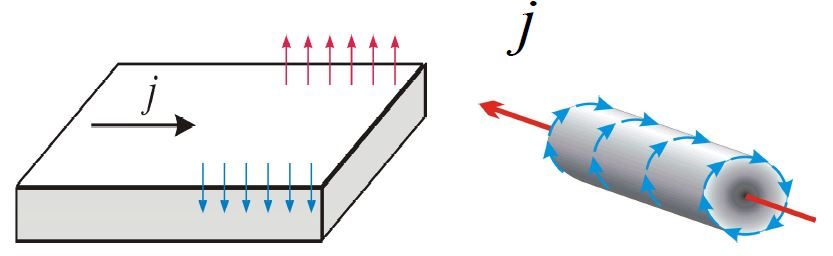
\includegraphics[width=0.5\textwidth]{pic/spin-hall}
\end{figure}

历史上有两个解释(来自\href{https://en.wikipedia.org/wiki/Spin_Hall_effect}{维基})。其一是说流动的电子会与材料中的杂质碰撞发生散射。根据自旋方向的不同,散射的方位角分布也会显示出差异,从而带有不同方向自旋的电子会逐渐弥散到相对的两侧。

第二种解释称这是材料的内禀属性,与杂质无关,它是由电子自旋--轨道相互作用引起的。在不对称的有效电场下因电子的自旋会产生额外的能量项,使得自旋不同的电子有不同的运动轨迹。这和经典力学的马格努斯效应(旋转的乒乓球在空气中轨迹发生偏转)有相似之处。

\end{enumerate}
\newpage
\begin{center}
    \Large{\textbf{第六、八章作业及小测解答}}
\end{center}

第六章“自旋与全同粒子体系”对应曾谨言书上第九章
\begin{enumerate}[label=\textbf{6.\arabic*}, listparindent=\parindent]

\setcounter{enumi}{1}
\item
{\color{red}\textbf{讨论:}}

本题还可以用作业3.22(即《解答》5.10)中“旋转”的观点去理解。在$\sigma_z$表象中,$\sigma_z$本征态写作$\psi_{\frac{1}{2}}=\smqty(1\\0)$, $\psi_{-\frac{1}{2}}=\smqty(0\\1)$。将$\vec{e}_z$方向转至$\vec{n}=(\sin\theta\cos\varphi,\sin\theta\sin\varphi,\cos\theta)$,可先沿着$y$轴转$\theta$角,再沿着$z$轴转$\varphi$角。因此根据作业3.22可知$\vec{\sigma\cdot n}$
的本征态为
\[\phi_{\pm\frac{1}{2}}=\ee{-\im\hat{s}_z\varphi/\hbar}\,\ee{-\im\hat{s}_y\theta/\hbar}\,\psi_{\pm\frac{1}{2}}\]
这个公式首先是用自旋$\frac{1}{2}$的角动量算符$\hat{\vec{s}}$写出的。我们知道$\hat{\vec{s}}=\frac{\hbar}{2}\vec{\sigma}$。又因为有
\[\ee{\im\lambda\vec{\sigma\cdot n}} =\cos\lambda + \im\sin\lambda(\vec{\sigma\cdot n})\]
(注意这是对自旋$\frac{1}{2}$特有的公式。)所以
\alg{\ee{-\im\hat{s}_z\varphi/\hbar}\,\ee{-\im\hat{s}_y\theta/\hbar} 
= \ee{-\im\frac{\varphi}{2}\sigma_z}\,\ee{-\im\frac{\theta}{2}\sigma_y}= \mqty(\ee{-\im\frac{\varphi}{2}} & \\ & \ee{\im\frac{\varphi}{2}})
\mqty(\cos\frac{\theta}{2} & -\sin\frac{\theta}{2}\\ \sin\frac{\theta}{2}&\cos\frac{\theta}{2})= \mqty(\cos\frac{\theta}{2}\ee{-\im\frac{\varphi}{2}} & -\sin\frac{\theta}{2}\ee{-\im\frac{\varphi}{2}}\\ \sin\frac{\theta}{2}\ee{\im\frac{\varphi}{2}}&\cos\frac{\theta}{2}\ee{\im\frac{\varphi}{2}})}
将其作用在$\psi_{\pm\frac{1}{2}}$上有
\[\phi_{\frac{1}{2}}=\mqty(\cos\frac{\theta}{2}\ee{-\im\frac{\varphi}{2}} \\ \sin\frac{\theta}{2}\ee{\im\frac{\varphi}{2}}),\quad \phi_{-\frac{1}{2}}=\mqty(-\sin\frac{\theta}{2}\ee{-\im\frac{\varphi}{2}}\\\cos\frac{\theta}{2}\ee{\im\frac{\varphi}{2}})\]
也可以验证$\sigma_z$的变换(注意$\sigma_z$右边e指数的顺序)
\alg{\ee{-\im\frac{\varphi}{2}\sigma_z}\,\ee{-\im\frac{\theta}{2}\sigma_y}\,\sigma_z\,\ee{\im\frac{\theta}{2}\sigma_y}\,\ee{\im\frac{\varphi}{2}\sigma_z}
&= \mqty(\cos\frac{\theta}{2}\ee{-\im\frac{\varphi}{2}} & -\sin\frac{\theta}{2}\ee{-\im\frac{\varphi}{2}}\\ \sin\frac{\theta}{2}\ee{\im\frac{\varphi}{2}}&\cos\frac{\theta}{2}\ee{\im\frac{\varphi}{2}})
\mqty(1&\\&-1)
\mqty(\cos\frac{\theta}{2}\ee{\im\frac{\varphi}{2}} & \sin\frac{\theta}{2}\ee{-\im\frac{\varphi}{2}}\\ -\sin\frac{\theta}{2}\ee{\im\frac{\varphi}{2}}&\cos\frac{\theta}{2}\ee{-\im\frac{\varphi}{2}})\\
&= \mqty(\cos\theta & \sin\theta\ee{-\im\varphi}\\ \sin\theta\ee{\im\varphi} & -\cos\theta) = \vec{\sigma\cdot n}}
请同学们自行验算上面的式子。

\setcounter{enumi}{4}
\item
【另解】

\noindent(b) 可直接利用$V_T(r)S_{12} = V_T(r)\,(6S_n^2-2\vec{S}^2)$以及对$\vec{S}$的自旋单态有
\[S_n\ket{\psi;00} = 0,\quad \vec{S}\ket{\psi;00}=0\]
因此张量势$V_T(r)S_{12}\ket{\psi;00}\equiv 0$,
故张量力恒为0。

\setcounter{enumi}{11}
\item
{\color{red}\textbf{讨论:}}

可以继续6.2题对一般的角动量旋转做一讨论,对任意角动量算符$\hl$ (满足$[\hat{l}_i,\hat{l}_j]=\im\eijk\hat{l}_k$),有
\[\ee{-\im\theta \vec{n\cdot }\hat{\vec{l}}/\hbar}\,(\vnt\vec{\cdot}\hl)\,\ee{\im\theta \vec{n\cdot}\hat{\vec{l}}/\hbar} = \vnt'\vec{\cdot}\hl\]
解读为沿$\vnt$方向的角动量 (即$\vnt\vec{\cdot}\hl$) 经旋转后变成沿$\vnt'$方向的角动量,$\vnt'$单位矢量是将$\vnt$以$\vec{n}$为转轴逆时针旋转$\theta$角后得到的。根据几何知识,将$\vnt$在$\vec{n}$上投影大小为$\vn\vec{\cdot}\vnt$,在其法平面上投影(矢量)为$(\vn\vec{\times}\vnt)\vec{\times}\vn$,法平面上与之垂直等大的矢量为$\vn\vec{\times}\vnt$ (还需注意有前后两个方向),故
\[\vn_l'=(\vn\vec{\cdot}\vnt)\vn+\qty((\vn\vec{\times}\vnt)\vec{\times}\vn)\cos\theta + (\vn\vec{\times}\vnt)\sin\theta\]
在本章处理的$\frac{1}{2}$自旋中,$\hl=\frac{\hbar}{2}\vec{\sigma}$,$\ee{\im\lambda\vec{n\cdot\sigma}} = \ee{\im(2\lambda)\vec{n\cdot }\hl/\hbar}$,因此对本题而言,最直接的等式是
\[\ee{\im\lambda \vec{n\cdot\sigma}}\,(\vnt\vec{\cdot\sigma})\,\ee{-\im\lambda \vec{n\cdot\sigma}} = \qty[(\vn\vec{\cdot}\vnt)\vn+\qty((\vn\vec{\times}\vnt)\vec{\times}\vn)\cos(-2\lambda) + (\vn\vec{\times}\vnt)\sin(-2\lambda)]\vec{\cdot \sigma}\]
如何将该式化为题中的式子?容易利用爱因斯坦记号展开证明以下恒等式
\[(\vA\btimes\vB)\bcdot\vC = -(\vA\btimes\vC)\bcdot\vB,\quad\qty[(\vA\btimes\vB)\btimes\vC]\bcdot\vD = \qty[(\vA\btimes\vD)\btimes\vC]\bcdot\vB\]
因此可将右式的$\vec{\sigma}$与$\vnt$交换,并改变第三项的符号。两边同时约去$(\vnt\bcdot)$即为题中要证的式子。

\setcounter{enumi}{22}
\item
{\color{red}\textbf{讨论:}}

此类问题都可以用6.24解法二的方法,分$j=l\pm\frac{1}{2}$两类情况分别计算结果。前提是牢记非耦合表象$(\vec{l}^2,m_l,m_s)$本征态到耦合表象$(\vec{l}^2,\vec{j}^2,m_j)$本征态的变换系数:
\[\ket{l,j=l+\tfrac{1}{2},m_j}=\mqty(\sqrt{\frac{l+m+1}{2l+1}}\Y_{lm}\\\sqrt{\frac{l-m}{2l+1}}\Y_{l,m+1}),\quad
\ket{l,j=l-\tfrac{1}{2},m_j}=\mqty(-\sqrt{\frac{l-m}{2l+1}}\Y_{lm}\\\sqrt{\frac{l+m+1}{2l+1}}\Y_{l,m+1})
\]
请大家练习直接用上式推导本题结果。

\setcounter{enumi}{30}
\item

\noindent (1) 设单位径矢量$\hr=(\sin\theta\cos\varphi,\,\sin\theta\sin\varphi,\,\cos\theta)$,则 
\[h=\frac{1}{2}\mqty(\cos\theta & \sin\theta\ee{-\im\varphi}\\ \sin\theta\ee{\im\varphi} & -\cos\theta)\]
之后参见6.2题。

\noindent (2) 根据$\ee{\im\lambda\vec{\sigma\cdot n}} =\cos\lambda + \im\sin\lambda(\vec{\sigma\cdot n})$,代入$\lambda=\frac{\pi}{2}$:
\[\ee{\im\pi h}=\ee{-\im\frac{\pi}{2}\vec{\sigma\cdot n}}=\cos\frac{\pi}{2}+\im(2h)\sin\frac{\pi}{2}=2\im h\]

\noindent (3) 由$h^2=\frac{1}{4}$可知$h^{-1}=4h$,
\[\tilde{F}=U^{-1}FU=h^{-1}F h=4hFh\]
而
\[F+4h\,[F,\,h] = F+4hFh-4h^2F = F+4hFh-F = 4hFh\]
两式相等.

\noindent (4) 用爱因斯坦符号推导最为方便。以下用$\vec{n}$代替单位径矢,$\vec{n}=(n_x,n_y,n_z)$。{\color{red}推导中最常用的两个式子是:}
\alg{&\sigma_i\sigma_j = \delta_{ij}+\im\eijk\sigma_k\quad\text{(用于减少$\sigma$的个数。最后每项只含0或1个$\sigma$)}\\
&\eijk\varepsilon_{ijl} = 2\,\delta_{kl},\quad\varepsilon_{ijk}\varepsilon_{ilm} = \delta_{jl}\delta_{km}-\delta_{jm}\delta_{kl},\quad\text{(用于所并两个$\varepsilon$)}}
总结一下基本思想:用第一行等式不断减少$\sigma$个数,但会增加$\varepsilon$,随后用第二行等式将两个$\varepsilon$缩并进行化简。遇到有$l$的项需想办法构造对易式(如$[l_i,\,n_j]$, $[l_i,\,\sigma_jn_j]$等)将其去除。
\begin{enumerate}
    \item 计算$\tilde{\vec{s}}$。我们以$\tilde{\vec{s}}=4h\vec{s}h = \frac{1}{2}(\vec{\sigma\cdot n})\,\vec{\sigma}\,(\vec{\sigma\cdot n })$为出发点,
    考虑其$i$分量(\,{\color{red}\underline{下划线}}表示每一步推导要点):
    \alg{\tilde{s}_i=\tfrac{1}{2}(\underline{\sigma_j}n_j)\,\underline{\sigma_i}\,(\sigma_l n_l)&=\tfrac{1}{2}(\delta_{ij}-\im\eijk\underline{\sigma_k})\,\underline{\sigma_l}n_jn_l\\
    &= \tfrac{1}{2}n_i\sigma_ln_l - \tfrac{1}{2}\im\underline{\eijk}(\delta_{kl}+\im\underline{\eklm}\sigma_m)n_jn_l\\
    &= \tfrac{1}{2}n_i\sigma_ln_l - \tfrac{1}{2}\im\eijk n_jn_k+\tfrac{1}{2}(\delta_{il}\delta_{jm}-\delta_{im}\delta_{jl})\sigma_mn_jn_l\\
    &= \tfrac{1}{2}n_i\sigma_ln_l-0 +\tfrac{1}{2}\sigma_jn_jn_i - \tfrac{1}{2}\sigma_in_jn_j\\
    &= n_i\sigma_j n_j - \tfrac{1}{2}\sigma_i = \qty[\vec{n}\,(\vec{\sigma\cdot}\hr)-\tfrac{1}{2}\vec{\sigma}]_i}
    因此$\tilde{\vec{s}}=-\vec{s}+2\,\vn h$.
    
    \item 计算$\tilde{\vec{l}}$。首先,
    \alg{[l_i,\,n_j]&=[l_i,\,\tfrac{r_j}{r}]=[l_i,\,r_j]\,\tfrac{1}{r}+r_j\,[l_i,\,\tfrac{1}{r}]=\im\eijk r_k\tfrac{1}{r}+0=\im\eijk n_k\\   [l_i,\,\vec{\sigma\cdot n}]&=\qty[l_i,\,\sigma_jn_j] = [l_i,\sigma_j]\,n_j+\sigma_j\,[l_i,\,n_j]= 0+\sigma_j\im\eijk n_k = \im\eijk \sigma_jn_k}
    用(3)问的结论:
    \alg{\tilde{l}_i=l_i+(\vec{\sigma\cdot n})\,[l_i,\,\vec{\sigma\cdot n}]
    &= l_i+\underline{\sigma_l} n_l\,(\im\eijk\underline{\sigma_j} n_k) \\
    &= l_i+\im\underline{\eijk}\,(\delta_{jl}+\im\underline{\varepsilon_{ljm}}\sigma_m)n_ln_k\\
    &= l_i+\im\eijk n_j n_k - (\delta_{km}\delta_{il}-\delta_{kl}\delta_{im})\,\sigma_m n_l n_k\\
    &= l_i +0 -\sigma_kn_in_k+\sigma_in_kn_k = l_i-n_i\,(\vec{\sigma\cdot n})+\sigma_i}
    最后一步用到$n_kn_k=1$。因此$\tilde{\vec{l}}=\vec{l}-2\,\vec{n}h+2\vec{s}$.
    \item 计算$\tilde{\vec{j}}$。
    \[\tilde{\vec{j}}=\tilde{\vec{l}}+\tilde{\vec{s}}= \vec{l}-2\,\vec{n}h+2\vec{s}-\vec{s}+2\,\vn h =\vec{l}+\vec{s}= \vec{j}\]
    说明$[\vec{j},\,h]=0$.
    若直接推导:
    \[[j_i,\,\vec{\sigma\cdot n}]=[l_i,\,\vec{\sigma\cdot n}]+\tfrac{1}{2}[\sigma_i,\,\sigma_jn_j]=\im\eijk\sigma_jn_k+\tfrac{1}{2}(2\im\eijk\sigma_k)n_j = 0\]
    
    \item 计算$\tilde{\vec{l}}^2$。{\color{red}请注意题目答案有误。}我们提供三种解法,前两种善用前面小问的结果,稍显简洁;第三种暴力求解。
    
    【法一】
    直接对(b)结果进行平方:$\tilde{\vec{l}}^2=(\tilde{\vec{l}})^2=(l_i+\sigma_i-n_i\sigma_kn_k)(l_i+\sigma_i-n_i\sigma_ln_l)$。注意爱因斯坦记号要求每个下表必须只能出现1或2次, 2次代表指标缩并,出现多于2次是违规的。故上面用了$k$和$l$两组下标。
    展开为
    \[\tilde{\vec{l}}^2 = l_il_i+\sigma_i\sigma_i+ n_in_i\sigma_kn_k\sigma_ln_l+
    2\,l_i\sigma_i-2\,l_in_i\sigma_kn_k - 2\,\sigma_in_i\sigma_kn_k \]
    上式代入
    \[l_in_i=0,\quad \sigma_i\sigma_i = 3,\quad\sigma_in_i\sigma_jn_j=(\vec{\sigma\cdot n})^2=1\]
    得到$\tilde{\vec{l}}^2=l_il_i+3+1+2\,l_i\sigma_i-0-2 = \vec{l}^2+4\,(\vec{s\cdot l})+2$.
    
    【法二】善用(b)的结果。将所求化为
    \alg{\tilde{\vec{l}}^2=\vec{l}^2+(\vec{\sigma\cdot n})\,[\vec{l}^2,\,\vec{\sigma\cdot n}] &= \vec{l}^2+\underline{(\vec{\sigma\cdot n})}\,\underline{l_i}\,[l_i,\,\vec{\sigma\cdot n}]+(\vec{\sigma\cdot n})\,[l_i,\,\vec{\sigma\cdot n}]\,l_i\\
    &= \vec{l}^2+l_i\,(\vec{\sigma\cdot n})\,[l_i,\,\vec{\sigma\cdot n}]-[l_i,\,\vec{\sigma\cdot n}][l_i,\,\vec{\sigma\cdot n}]+(\vec{\sigma\cdot n})\,[l_i,\,\vec{\sigma\cdot n}]\,l_i}
    由(b)知$(\vec{\sigma\cdot n})[l_i,\,\vec{\sigma\cdot n}]=\sigma_i+n_i\sigma_kn_k$,且$[l_i,\,\vec{\sigma\cdot n}]=\im\eijk\sigma_jn_k$,代入有
    \alg{\tilde{\vec{l}}^2 &=\vec{l}^2+l_i\,(\sigma_i+n_i\sigma_kn_k)-(\im\underline{\eijk}\sigma_jn_k)(\im\underline{\varepsilon_{ilm}}\sigma_ln_m)+(\sigma_i+n_i\sigma_kn_k)\,l_i\\
    &= \vec{l}^2+(l_i\sigma_i+0)-\qty(-(\delta_{jl}\delta_{km}-\delta_{jm}\delta_{kl})\,\sigma_j\sigma_ln_kn_m)+(\sigma_il_i+0)\\
    &= \vec{l}^2+l_i\sigma_i+(\sigma_j\sigma_jn_kn_k-\sigma_jn_k\sigma_k\sigma_j)+l_i\sigma_i\\
    &= \vec{l}^2+l_i\sigma_i+(3-1)+l_i\sigma_i }
    故$\tilde{\vec{l}}^2= \vec{l}^2+4\,(\vec{s\cdot l})+2$。
    
    【法三】暴力求解。
    从$\tilde{\vec{l}}^2=\vec{l}^2+(\vec{\sigma\cdot n})\,[\vec{l}^2,\,\vec{\sigma\cdot n}]$出发,首先\;{\color{red} (注意到$l$和$\sigma$可交换,但$l$和$n$不可交换!)}
    \alg{[\vec{l}^2,\,\vec{\sigma\cdot n}]=[l_il_i,\,\sigma_jn_j] &= l_i\,[l_i,\,\sigma_jn_j]+[l_i,\,\sigma_jn_j]\,l_i = \im\eijk\sigma_j (l_in_k+n_kl_i) \\
    &= 2\im\eijk\sigma_j n_kl_i + \im\eijk\sigma_j\,[l_i,n_k]\\
    &= 2\im\eijk\sigma_j n_kl_i + \im\underline{\eijk}\sigma_j\,(\im\underline{\varepsilon_{ikl}}n_l)\\
    &= 2\im\eijk\sigma_j n_kl_i -(-2\,\delta_{jl}\sigma_jn_l) = 2\im\eijk\sigma_j n_kl_i+2\,\sigma_jn_j}
    因此
    \alg{\tilde{\vec{l}}^2 &= \vec{l}^2+(\underline{\sigma_l}n_l)\,\qty(2\im\eijk\underline{\sigma_j} n_kl_i+2\,\sigma_jn_j) \\
    &= \vec{l}^2+(\delta_{lj}+\im\underline{\varepsilon_{ljm}}\sigma_m)\,2\im\,\underline{\eijk} n_ln_kl_i + 2\,\sigma_ln_l\sigma_jn_j\\
    &= \vec{l}^2+2\im\,\eijk n_jn_kl_i -2\,(\delta_{km}\delta_{il}-\delta_{kl}\delta_{im})\,\sigma_mn_ln_kl_i+2\,\sigma_ln_l\sigma_jn_j\\
    &= \vec{l}^2+2\im\,\eijk n_jn_kl_i - 2\,\sigma_kn_in_kl_i + 2\,\sigma_in_kn_kl_i + 2\,\sigma_ln_l\sigma_jn_j}
    上式第二项$i,j$反称故为0;第三项交换$n_in_k$后因为有$n_il_i=\eijk r_ir_jp_k/r = 0$ (经典上理解:$\vec{n\cdot l}=0$, 同理也可证$l_in_i=0$)故为0。因此
    $\tilde{\vec{l}}^2 = \vec{l}^2+2\,\sigma_il_i+2=\vec{l}^2+4\,(\vec{s\cdot l})+2$即为所求.
    
    \item 求$\tilde{\vec{l}}\bcdot\tilde{\vec{s}}$。
    
    【法一】直接将(a), (b)结果相乘。有
    \alg{\tilde{l}_i\tilde{s}_i &= (l_i+\sigma_i-n_i\sigma_jn_j)(n_i\sigma_kn_k - \tfrac{1}{2}\sigma_i)\\
    &= (l_in_i\sigma_kn_k + \sigma_in_i\sigma_kn_k - n_in_i\sigma_jn_j\sigma_kn_k) + (-\tfrac{1}{2}l_i\sigma_i-\tfrac{1}{2}\sigma_i\sigma_i + \tfrac{1}{2}\sigma_in_i\sigma_jn_j)\\
    &= (0+1-1)+(-\tfrac{1}{2}l_i\sigma_i-\tfrac{3}{2}+\tfrac{1}{2}) = -\tfrac{1}{2}l_i\sigma_i-1}
    故$\tilde{\vec{l}}\bcdot\tilde{\vec{s}} = -\vec{l\cdot s}-1$.
    
    【法二】【法三】 可以用类似于(d)问的法二、法三的思想进行求解,请同学们自己练习推导。
\end{enumerate}
{\color{red}\textbf{注:}此题算错的同学很多,绝大多数同学没有发现答案有误。助教批改的不仔细,还请大家自己核查一遍过程。其中最容易出错的地方就是直接交换$l$和$n$算符,答案的失误似也与之有关。}

\end{enumerate}

第八章“电磁场中的粒子”对应曾谨言书上第七章
\begin{enumerate}[label=\textbf{8.\arabic*}, listparindent=\parindent]

\setcounter{enumi}{1}
\item
{\color{red}\textbf{注:}}恒磁场中粒子运动的朗道能级的求解还需掌握{\color{red}能级简并的特征}。请大家复习下这一部分内容。


\end{enumerate}

小测题目解答:
\begin{enumerate}[label=\textbf{6.\Alph*}, listparindent=\parindent]

\item 
\begin{enumerate}[listparindent=\parindent]
\item \emph{推导:$\ee{\im\theta \vec{\sigma\cdot n}}=\cos\theta+\im\sin\theta\vec{\sigma\cdot n}$.}

进行幂级数展开
\alg{\ee{\im\theta\vec{\sigma\cdot n}}=\sum_{n=0}^{\infty}\frac{1}{n!}(\im\theta\vec{\sigma\cdot n})^n}
由于
\[(\vec{\sigma\cdot n})^2 = \sigma_in_i\sigma_j n_j = (\delta_{ij}+\im\eijk\sigma_k)\,n_in_j = \delta_{ij}n_in_j = 1\]
故\[(\vec{\sigma\cdot n})^{2k}=1,\quad(\vec{\sigma\cdot n})^{2k+1}=\vec{\sigma\cdot n},\quad \text{$k$为整数}\]
\[\ee{\im\theta\vec{\sigma\cdot n}}=\sum_{k=0}^{\infty}\frac{1}{(2k)!}(-\im\theta)^{2k}+\sum_{k=0}^{\infty}\frac{1}{(2k+1)!}(-\im\theta)^{2k+1}(\vec{\sigma\cdot n})=\cos\theta + \im\sin\theta\,\vec{\sigma\cdot n}\]
证毕。

\item \emph{推导:$\Tr((\vec{\sigma\cdot A})(\vec{\sigma\cdot B})(\vec{\sigma\cdot C})) = 2\im\,(\vec{A\times B})\bcdot\vec{C}$,其中$\vA$, $\vB$, $\vC$为矢量.}

我们知道$(\vec{\sigma\cdot n})^2=1$,故无论多么复杂的$\vec{\sigma}$矩阵表达式都可以最终化为$A_0+B_0\,\vec{\sigma\cdot n}_0$的形式。这也可以从爱因斯坦记号的表示看出:因为有$\sigma_i\sigma_j=\delta_{ij}+\im\eijk\sigma_k$,总可以将两个$\sigma$缩并以减少1个$\sigma$矩阵,使得最后的每一项中都不含$\sigma$或只含1个$\sigma$矩阵。

为此可以将$\Tr(\cdot)$内部矩阵化简(下划线表示推导要点)
\alg{(\vec{\sigma\cdot A})(\vec{\sigma\cdot B})(\vec{\sigma\cdot C})&=\underline{\sigma_i}A_i\underline{\sigma_j}B_j\sigma_kC_k = (\delta_{ij}+\im\varepsilon_{ijl}\underline{\sigma_l})\underline{\sigma_k}A_iB_jC_k\\
&= \sigma_kA_iB_iC_k + \im\underline{\varepsilon_{ijl}}(\delta_{lk}+\im\underline{\varepsilon_{lkm}}\sigma_m)A_iB_jC_k\\
&= \sigma_kA_iB_iC_k + \im\varepsilon_{ijk}A_iB_jC_k - (\delta_{ik}\delta_{jm}-\delta_{im}\delta_{jk})\sigma_mA_iB_jC_k\\
&= \sigma_kA_iB_iC_k + \im\varepsilon_{ijk}A_iB_jC_k -\sigma_jA_iB_jC_i + \sigma_iA_iB_jC_j}
现在结果中每一项都含0个或1个$\sigma$。由于
\[\Tr(I)=2,\quad \Tr(\sigma_i)=0,\]
则只有不含$\sigma$项对矩阵的迹有贡献:\[\Tr((\vec{\sigma\cdot A})(\vec{\sigma\cdot B})(\vec{\sigma\cdot C}))=2\im\varepsilon_{ijk}A_iB_jC_k=2\im\,(\vec{A\times B})\bcdot\vec{C}.\]

\item \emph{化简:$\ee{\im\theta\vec{\sigma\cdot n}}\,(\vec{l\cdot \sigma})\,\ee{-\im\theta\vec{\sigma\cdot n}}$, 其中$\vec{n}=\frac{\vec{r}}{r}$为单位径向矢量,$\vec{l}$为轨道角动量.}

显然本题与6.12题很像。根据我们对6.12的几何诠释,相当于沿$\vec{l}$方向的自旋算符绕$\vec{n}$旋转。由于本题中$\vec{l}$方向是与$\vec{n}$垂直的,故不存在沿$\vn$方向的投影,问题还可以进一步简化。一个直接的想法是对6.12题结论等式两边点乘$\vec{l}$即可。但是,$\vec{l}$并不是普通矢量,它与$\vec{n}$是不对易的,满足
\[[l_i,\,n_j]=\im\varepsilon_{ijk}n_k.\]
故我们先将原式化为
\[\ee{\im\theta\vec{\sigma\cdot n}}\,l_i\sigma_i\,\ee{-\im\theta\vec{\sigma\cdot n}} = l_i\qty(\ee{\im\theta\vec{\sigma\cdot n}}\,\sigma_i\,\ee{-\im\theta\vec{\sigma\cdot n}})-[l_i,\,\ee{\im\theta\vec{\sigma\cdot n}}]\,\sigma_i\,\ee{-\im\theta\vec{\sigma\cdot n}}\]
第一项则回到6.12题的方法中来,可以得出 (请同学们补全过程)
\[l_i\qty(\ee{\im\theta\vec{\sigma\cdot n}}\,\sigma_i\,\ee{-\im\theta\vec{\sigma\cdot n}}) = l_i\sigma_i\,\cos2\theta +\eijk l_in_j\sigma_k\,\sin2\theta=(\vec{l\cdot \sigma})\cos2\theta+\vec{l}\bcdot(\vec{n\times\sigma})\,\sin2\theta\]

下面求第二项。首先求解对易关系
\[[l_i,\,\ee{\im\theta\sigma_jn_j}]=[l_i,\,\im\sin\theta\sigma_jn_j]=\im\sin\theta\,(\im\eijk \sigma_j n_k)\]
故
\alg{[l_i,\,\ee{\im\theta\sigma_jn_j}]\,\sigma_i &= -\sin\theta\,\eijk\underline{\sigma_j} n_k \underline{\sigma_i}\\
&= -\sin\theta\,\underline{\eijk}\,(\delta_{ij}-\im\underline{\varepsilon_{ijl}}\sigma_l)\,n_k \\
&= \im\sin\theta\,(2\delta_{kl})\,\sigma_ln_k=2\im\sin\theta\sigma_kn_k}
最后
\alg{[l_i,\,\ee{\im\theta\sigma_jn_j}]\,\sigma_i\,\ee{-\im\theta\sigma_ln_l}
&=2\im\sin\theta\,\sigma_kn_k\,(\cos\theta-\im\sin\theta\,\sigma_ln_l) \\
&= \im\,(\vec{n\cdot\sigma})\,\sin2\theta+2\sin^2\theta}
\end{enumerate}
最终结果为
\alg{\ee{\im\theta\vec{\sigma\cdot n}}\,l_i\sigma_i\,\ee{-\im\theta\vec{\sigma\cdot n}}&=
(\vec{l\cdot \sigma})\cos2\theta+\vec{l}\bcdot(\vec{n\times\sigma})\,\sin2\theta -\im\,(\vec{n\cdot\sigma})\,\sin2\theta-2\sin^2\theta\\
&= 
(\vec{l\cdot \sigma}+1)\,\cos2\theta+[\vec{l}\bcdot(\vec{n\times\sigma})-\im\,(\vec{n\cdot\sigma})]\,\sin2\theta-1.}


\noindent【法二】
可使用定理
\[\ee{A}\,B\,\ee{-A}=B+[A,B]+\frac{1}{2!}\qty[A,\,[A,B]]+\cdots\]
首先看看6.12题在本方法下的表现如何。可以归纳地证明 (通过算前几阶先找到规律):
\alg{&\Big[\underbrace{\im\theta\sigma_{j'}n_{j'},\cdots,[\im\theta\sigma_jn_j}_{\text{$2m+1$层}},\,\sigma_i]\Big]=(2\theta)^{2m+1}(-1)^{m}\,\varepsilon_{ijk}n_j\sigma_k,\quad&m=0,1,2,\cdots\\
&\Big[\underbrace{\im\theta\sigma_{j'}n_{j'},\cdots,[\im\theta\sigma_jn_j}_{\text{$2m$层}},\,\sigma_i]\Big]=(2\theta)^{2m}(-1)^{m}\,(\sigma_i-n_i\sigma_kn_k ),\quad&m=1,2,3,\cdots}
第0阶是一个例外,它显然等于$\sigma_i$。由此可以得到
\alg{\ee{\im\theta\vec{\sigma\cdot n}}\,\sigma_i\,\ee{-\im\theta\vec{\sigma\cdot n}}
&=(\sigma_i-n_i\sigma_kn_k )\,\cos2\theta + \varepsilon_{ijk}n_j\sigma_k\,\sin2\theta + n_i\sigma_kn_k\\
&=[(\vec{n\times\sigma})\btimes\vec{n}]_i\,\cos2\theta+(\vec{n\times\sigma})_i\,\sin2\theta+n_i(\vec{\sigma\cdot n})
}
最后一项正是为了补偿第0阶而加上的常数。可以验证这正是6.12的结果。

对于本例,用$l_i\sigma_i$替代$\sigma_i$,发现$l_i$会参与到对易关系当中。有
\alg{&\Big[\underbrace{\im\theta\sigma_{j'}n_{j'},\cdots,[\im\theta\sigma_jn_j}_{\text{$2m+1$层}},\,\sigma_i]\Big]=(2\theta)^{2m+1}(-1)^{m}\,(l_i\varepsilon_{ijk}n_j\sigma_k-\im\sigma_kn_k),\quad&m=0,1,2,\cdots\\
&\Big[\underbrace{\im\theta\sigma_{j'}n_{j'},\cdots,[\im\theta\sigma_jn_j}_{\text{$2m$层}},\,\sigma_i]\Big]=(2\theta)^{2m}(-1)^{m}\,(l_i\sigma_i-l_in_i\sigma_kn_k +1),\quad&m=1,2,3,\cdots}
可见两式各多出了最后一项,这是由于$l_i$参与对易关系带来的。当然第0阶仍是例外,它应等于$l_i\sigma_i$。再利用$l_in_i=0$将第2式第二项去掉,可以得到
\[\ee{\im\theta\vec{\sigma\cdot n}}\,l_i\sigma_i\,\ee{-\im\theta\vec{\sigma\cdot n}}=
(\vec{l\cdot \sigma}+1)\,\cos2\theta+[\vec{l}\bcdot(\vec{n\times\sigma})-\im\,(\vec{n\cdot\sigma})]\,\sin2\theta-1.\]

\item \emph{类氢原子的价电子处于$l=1$的态上,置于均匀磁场$\vec{B}=B\,\vec{e}_z$中。哈密顿量可表为(近似地)
\[\hH=\frac{\mu_BB}{\hbar}(\hat{L}_z+2\hat{S}_z)+\frac{2w}{\hbar^2}\hat{\vec{L}}\bcdot\hat{\vec{S}},\]
其中$w$为常数。$\hat{L}_z$的三个本征态为$\varphi_1$, $\varphi_0$, $\varphi_{-1}$; $\hat{S}_z$的本征函数为$\alpha$, $\beta$。二者本征态的乘积波函数为
\begin{align*}
\chi_1=\varphi_1\alpha,\quad \chi_3=\varphi_0\alpha,\quad \chi_5=\varphi_{-1}\alpha,\\
\chi_2=\varphi_1\beta,\quad \chi_4=\varphi_0\beta,\quad \chi_6=\varphi_{-1}\beta。
\end{align*}
\begin{enumerate}
    \item 证明:$\hat{\vec{L}}\bcdot\hat{\vec{S}}=\frac{1}{2}(\hat{L}_+\hat{S}_-+\hat{L}_-\hat{S}_+)+\hat{L}_z\hat{S}_z$。 $\hat{L}_\pm$, $\hat{S}_\pm$为轨道角动量与自旋的升降算符。
    \item 
    \[\begin{cases}
    \hH\chi_1=c_{11}\chi_1,&\hH\chi_6=c_{66}\chi_6,\\
    \hH\chi_2=c_{22}\chi_2+c_{23}\chi_3,&\hH\chi_3=c_{32}\chi_2+c_{33}\chi_3,\\
    \hH\chi_4=c_{44}\chi_4+c_{45}\chi_5,&\hH\chi_5=c_{54}\chi_4+c_{55}\chi_5
    \end{cases}\]
    试求出上述$c_{ij}$。
    \item 对$\mu_B=\varepsilon\ll w$和$\varepsilon \gg w$求出$\hH$的本征值。
\end{enumerate}}

\noindent【解】本题为$l=1$与$s=\frac{1}{2}$角动量的耦合。可画出下图帮助理解。
\begin{figure}[!ht]
    \centering
    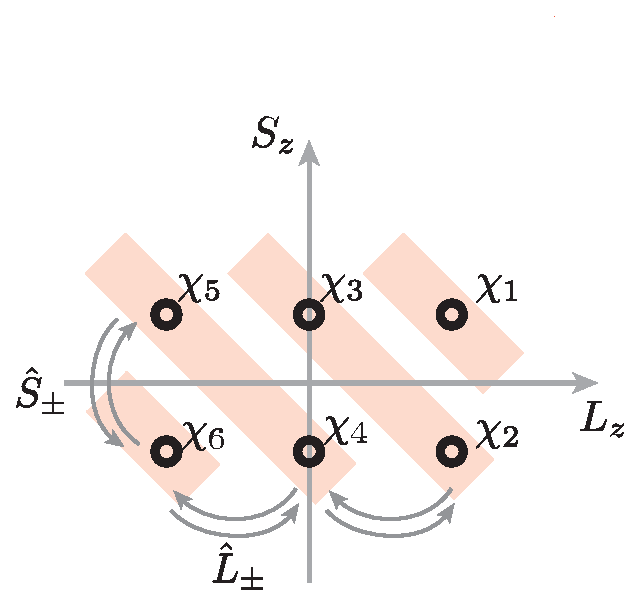
\includegraphics[width=0.4\textwidth]{pic/ls_couple.eps}
\end{figure}
\begin{enumerate}[listparindent=\parindent]
    \item 将$\hL_x=\frac{1}{2}(\hL_++\hL_-)$, $\hL_y=\frac{1}{2\im}(\hL_+-\hL_-)$代入,$\hS_x,\,\hS_y$同理,有
    \[\hat{\vec{L}}\bcdot\hat{\vec{S}}=\frac{1}{4}(\hL_++\hL_-)(\hS_++\hS_-)-\frac{1}{4}(\hL_+-\hL_-)(\hS_+-\hS_-)+\hL_z\hS_z = \frac{1}{2}(\hL_+\hS_-+\hL_-\hS_+)+\hL_z\hS_z\]
    证毕。
    
    \item 分析上问$\hat{\vec{L}}\bcdot\hat{\vec{S}}$的结果,发现若将它作用在非耦合表象的本征态$\ket{L_z,S_z}$(也即图中的每个圆点)上,结果中只会有$\ket{L_z+1,\,S_z-1}$, $\ket{L_z-1,\,S_z+1}$, $\ket{L_z,\,S_z}$这三种成分,也即不会脱离每条浅红色的区域。这是显然的,因为$\hat{\vec{L}}\bcdot\hat{\vec{S}}$与$\hat{J}_z=\hL_z+\hS_z$对易,故不会改变$J_z$的值。考虑到升降算符的作用效果为
    \[\hL_+\ket{-1,S_z}=\sqrt{2}\hbar\ket{0,S_z},\quad\hL_+\ket{0,S_z}=\sqrt{2}\hbar\ket{1,S_z}\]
    \[\hS_+\ket{L_z,-\tfrac{1}{2}}=\hbar\ket{L_z,\tfrac{1}{2}}\]
    将
    \[\hH = \frac{\varepsilon}{\hbar}(\hL_z+2\hS_z)+\frac{w}{\hbar^2}(\hL_+\hS_-+\hL_-\hS_+)+\frac{2w}{\hbar^2}\,\hL_z\hS_z\]
    分别作用到$\chi_1$到$\chi_6$上,可以得到
    \[\begin{cases}
    \hH\chi_1 = \varepsilon(1+2\cdot\frac{1}{2})\,\chi_1+2w\cdot1\cdot\frac{1}{2}\,\chi_1=(2\varepsilon+w)\,\chi_1\\
    \hH\chi_6 =\varepsilon(-1-2\cdot\frac{1}{2})\,\chi_6+2w\cdot(-1)\cdot\qty(-\frac{1}{2})\,\chi_6=(-2\varepsilon+w)\,\chi_6\\
    \hH\chi_2 =\varepsilon(1-2\cdot\frac{1}{2})\,\chi_2+\sqrt{2}w\,\chi_3+2w\cdot1\cdot\qty(-\frac{1}{2})\,\chi_2=-w\,\chi_2+\sqrt{2}w\,\chi_3\\
    \hH\chi_3 =\varepsilon(0+2\cdot\frac{1}{2})\,\chi_3+\sqrt{2}w\,\chi_2+2w\cdot0\cdot\frac{1}{2}\,\chi_3=\sqrt{2}w\,\chi_2+\varepsilon\,\chi_3\\
    \hH\chi_4 =\varepsilon(0-2\cdot\frac{1}{2})\,\chi_4+\sqrt{2}w\,\chi_5+2w\cdot0\cdot\qty(-\frac{1}{2})\,\chi_2=-\varepsilon\,\chi_4+\sqrt{2}w\,\chi_5\\
    \hH\chi_5 =\varepsilon(-1+2\cdot\frac{1}{2})\,\chi_5+\sqrt{2}w\,\chi_4+2w\cdot(-1)\cdot\frac{1}{2}\,\chi_5=\sqrt{2}w\,\chi_4-w\,\chi_5
    \end{cases}\]
    核对以上结果即可得到$c_{ij}$。
    \item 以$(\chi_1,\chi_2,\chi_3,\chi_4,\chi_5,\chi_6)$为基底写出$\hH$矩阵形式,由(b)知它在$(\chi_1)$, $(\chi_6)$, $(\chi_2,\chi_3)$, $(\chi_4,\chi_5)$上是块对角化的。作用在$\chi_1$上本征值为$2\varepsilon+w$;在$\chi_6$上本征值为$-2\varepsilon+w$。
    
    在$(\chi_2,\chi_3)$上局域矩阵为
    \[H_{23} = \mqty(-w&\sqrt{2}w\\\sqrt{2}w&\varepsilon),\]
    对角化$\abs{H_{23}-\lambda I}=(-w-\lambda)(\varepsilon-w)-2w^2=0$, 得到
    \[\lambda = \frac{-w+\varepsilon \pm\sqrt{9w^2+2w\varepsilon+\varepsilon^2}}{2}\]
    在$\varepsilon\ll w$时近似为$\lambda\approx\frac{1}{2}(-w+\varepsilon\pm 3w(1+\frac{\varepsilon}{9w}))=w+\frac{2}{3}\varepsilon$或$-2w+\frac{1}{3}\varepsilon$,在$\varepsilon\gg w$时近似为
    $\lambda\approx\frac{1}{2}(\varepsilon-w\pm\varepsilon(1+\frac{w}{\varepsilon}))=\varepsilon$或$-w$。
    
    在$(\chi_4,\chi_5)$上局域矩阵为
    \[H_{45} = \mqty(-\varepsilon&\sqrt{2}w\\\sqrt{2}w&-w),\]
    对角化$\abs{H_{45}-\lambda I}=(-\varepsilon-w)(-w-\lambda)-2w^2=0$, 得到
    \[\lambda = \frac{-w-\varepsilon \pm\sqrt{9w^2-2w\varepsilon+\varepsilon^2}}{2}\]
    在$\varepsilon\ll w$时近似为$\lambda\approx\frac{1}{2}(-w-\varepsilon\pm 3w(1-\frac{\varepsilon}{9w}))=w-\frac{2}{3}\varepsilon$或$-2w-\frac{1}{3}\varepsilon$,在$\varepsilon\gg w$时近似为
    $\lambda\approx\frac{1}{2}(-\varepsilon-w\pm\varepsilon(1-\frac{w}{\varepsilon}))=-w$或$-\varepsilon$。
    
    综上,在$\varepsilon\ll w$时,本征值为$w\pm2\varepsilon$, $w\pm\frac{2}{3}\varepsilon$, $-2w\pm\frac{1}{3}\varepsilon$;在$\varepsilon\gg w$时,本征值为$2\varepsilon+w$, $\varepsilon$, $-w$, $-w$, $-\varepsilon$, $-2\varepsilon+w$.
\end{enumerate}
\end{enumerate}


\end{document}
